\documentclass[11pt]{book}
\oddsidemargin 0in
\evensidemargin 0in
\marginparwidth 0in
\textheight 8in
\textwidth 6.5in
\topmargin 0in
\usepackage{amssymb,amsmath,amsthm,fancyhdr,supertabular,longtable,hhline}
\usepackage{colortbl}
\usepackage{import, multicol,boxedminipage}
\usepackage{chapterfolder}
\usepackage[metapost,truebbox]{mfpic}
\usepackage[pdflatex]{graphicx}
\usepackage{makeidx}
\usepackage[colorlinks, hyperindex, plainpages=false, linkcolor=blue, urlcolor=blue, pdfpagelabels]{hyperref}
\usepackage[all]{hypcap}
\usepackage{cancel}
\usepackage{sectsty}
\usepackage{textcomp}
\allsectionsfont{\mdseries \scshape}
\definecolor{ResultColor}{gray}{0.9}
\theoremstyle{definition}  % this prevents the text in definitions, theorems, and corollaries from being italicized
\newtheorem{defn}{Definition}[chapter]
\newtheorem{thm}{Theorem}[chapter]
\newtheorem{cor}[thm]{Corollary}
\newtheorem{eqn}{Equation}[chapter]
\newtheorem{ex}{Example}[section]
\setlength{\parindent}{0in}
\newcommand{\bbm}{\begin{boxedminipage}{6.41in}}
\newcommand{\ebm}{\end{boxedminipage}}
\newcounter{HW}
\newcounter{HWindent}

\begin{document}

\chapter{\sc Rational Functions}

\section{Introduction to Rational Functions}

\mfpicnumber{1}
\opengraphsfile{IntroRational}

\setcounter{footnote}{0}

\label{IntroRational}

If we add, subtract or multiply polynomial functions according to the function arithmetic rules defined in Section \ref{FunctionArithmetic}, we will produce another polynomial function. If, on the other hand, we divide two polynomial functions, the result may not be a polynomial.  In this chapter we study \index{rational functions} \textbf{rational functions} - functions which are ratios of polynomials.

\smallskip

\colorbox{ResultColor}{\bbm

\begin{defn}  \label{rationalfunction} A \textbf{rational function} is a function which is the ratio of polynomial functions.  Said differently, $r$ is a rational function if it is of the form \index{function ! rational}

\[ r(x) = \dfrac{p(x)}{q(x)},\]

where $p$ and $q$ are polynomial functions.\footnote{According to this definition, all polynomial functions are also  rational functions. (Take $q(x) = 1$).}

\end{defn}

\ebm}

\smallskip

As we recall from Section \ref{FunctionNotation}, we have domain issues anytime the denominator of a fraction is zero.  In the example below, we review this concept as well as some of the arithmetic of rational expressions.

\begin{ex} \label{ratfuncex} Find the domain of the following rational functions.  Write them in the form $\frac{p(x)}{q(x)}$ for polynomial functions $p$ and $q$ and simplify.

\begin{multicols}{2}
\begin{enumerate}

\item  $f(x) = \dfrac{2x-1}{x+1}$
\item  $g(x) = 2 - \dfrac{3}{x+1}$

\setcounter{HW}{\value{enumi}}
\end{enumerate}
\end{multicols}

\begin{multicols}{2}
\begin{enumerate}
\setcounter{enumi}{\value{HW}}

\item  $h(x) = \dfrac{2x^2-1}{x^2-1} - \dfrac{3x-2}{x^2-1}$
\item  $r(x) = \dfrac{2x^2-1}{x^2-1} \div \dfrac{3x-2}{x^2-1}$

\setcounter{HW}{\value{enumi}}
\end{enumerate}
\end{multicols}

{\bf Solution.}

\begin{enumerate}

\item To find the domain of $f$, we proceed as we did in Section \ref{FunctionNotation}: we find the zeros of the denominator and exclude them from the domain.  Setting $x+1=0$ results in  $x=-1$. Hence, our domain is  $(-\infty, -1) \cup (-1,\infty)$.  The expression $f(x)$ is already in the form requested and when we check for common factors among the numerator and denominator we find none, so we are done.

\item  Proceeding as before, we determine the domain of $g$ by solving $x+1=0$.  As before, we find the domain of $g$ is $(-\infty, -1) \cup (-1,\infty)$.  To write $g(x)$ in the form requested, we need to get a common denominator 

\[ \begin{array}{rclclcl}

g(x) & = & 2 - \dfrac{3}{x+1} & = & \dfrac{2}{1} - \dfrac{3}{x+1} & = & \dfrac{(2)(x+1)}{(1)(x+1)} - \dfrac{3}{x+1} \\ [.15in]
     & = & \dfrac{(2x+2) - 3}{x+1} & = & \dfrac{2x-1}{x+1} & & \\ \end{array} \]

This formula is now completely simplified.


\item  The denominators in the formula for $h(x)$ are both $x^2-1$ whose zeros are  $x = \pm 1$.  As a result, the domain of $h$ is $(-\infty, -1) \cup (-1,1) \cup (1, \infty)$.  We now proceed to simplify $h(x)$.  Since we have the same denominator in both terms, we subtract the numerators.  We then factor the resulting numerator and denominator, and cancel out the common factor.

\[ \begin{array}{rclcl}

h(x) & = & \dfrac{2x^2-1}{x^2-1} - \dfrac{3x-2}{x^2-1} & = & \dfrac{\left(2x^2-1\right) - \left(3x-2\right)}{x^2-1} \\ [.15in]
     & = & \dfrac{2x^2-1 - 3x+2}{x^2-1} & = &  \dfrac{2x^2 - 3x+1}{x^2-1} \\ [.15in]
     & = & \dfrac{(2x-1)(x-1)}{(x+1)(x-1)} & = & \dfrac{(2x-1)\cancel{(x-1)}}{(x+1)\cancel{(x-1)}} \\ [.15in]
     & = & \dfrac{2x-1}{x+1} & & \\
\end{array} \]

\item  To find the domain of $r$, it may help to temporarily rewrite $r(x)$ as

\[ r(x) = \dfrac{\dfrac{2x^2-1}{x^2-1} }{\dfrac{3x-2}{x^2-1}\vphantom{\left(\dfrac{X}{X}\right)}}\]

We need to set all of the denominators equal to zero which means we need to solve not only  $x^2-1= 0$, but also $\frac{3x-2}{x^2-1}=0$.  We find $x = \pm 1$ for the former and $x= \frac{2}{3}$ for the latter.  Our domain is $(-\infty, -1) \cup \left(-1,\frac{2}{3}\right) \cup \left(\frac{2}{3},1\right) \cup (1, \infty)$.  We simplify $r(x)$ by rewriting the division as multiplication by the reciprocal and then by canceling the common factor

\[ \begin{array}{rclclcl}

r(x) & = & \dfrac{2x^2-1}{x^2-1} \div \dfrac{3x-2}{x^2-1} & = & \dfrac{2x^2-1}{x^2-1} \cdot \dfrac{x^2-1}{3x-2} & = & \dfrac{\left(2x^2-1\right)\left(x^2-1\right)}{\left(x^2-1\right)(3x-2)} \\ [.15in]
     & = & \dfrac{\left(2x^2-1\right)\cancel{\left(x^2-1\right)}}{\cancel{\left(x^2-1\right)}(3x-2)} & = & \dfrac{2x^2-1}{3x-2} & & \\ 
\end{array}\]

\end{enumerate}

\end{ex}

\vspace{-.35in} \qed

\medskip

A few remarks about Example \ref{ratfuncex} are in order. Note that the expressions for $f(x)$, $g(x)$ and $h(x)$ work out to be the same.  However, only two of these functions are actually equal.  Recall that functions are ultimately sets of ordered pairs,\footnote{You should review Sections \ref{Relations} and \ref{IntrotoFunctions} if this statement caught you off guard.} so for two functions to be equal, they need, among other things, to have the same domain.  Since $f(x) = g(x)$ and $f$ and $g$ have the same domain, they are equal functions.  Even though the formula $h(x)$ is the same as $f(x)$, the domain of $h$ is different than the domain of $f$, and thus they are different functions.  

\medskip

We now turn our attention to the graphs of rational functions. Consider the function $f(x) = \frac{2x-1}{x+1}$ from Example \ref{ratfuncex}.  Using a graphing calculator, we obtain

\medskip

\centerline{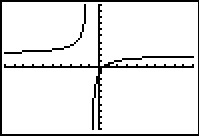
\includegraphics[width=2in]{./RationalsGraphics/Rationals01.jpg}}

\medskip

Two behaviors of the graph are worthy of further discussion.  First, note that the graph appears to `break' at $x=-1$. We know from our last example that $x=-1$ is not in the domain of $f$ which means $f(-1)$ is undefined. When we make a table of values to study the behavior of $f$ \textit{near} $x=-1$ we see that we can get `near' $x=-1$ from two directions.  We can choose values a little less than $-1$, for example $x=-1.1$, $x=-1.01$, $x=-1.001$, and so on.  These values are said to `approach $-1$ from the \textit{left}.'  Similarly, the values $x=-0.9$, $x=-0.99$, $x=-0.999$, etc., are said to `approach $-1$ from the \textit{right}.'  If we make two tables, we find that the numerical results confirm what we see graphically.

\begin{center}
\begin{tabular}{cc}

$\begin{array}{|r||c|c|}  \hline

  x & f(x) & (x,f(x)) \\ \hline
 -1.1 & 32 & (-1.1, 32) \\  \hline
 -1.01 & 302 & (-1.01, 302) \\  \hline 
 -1.001 & 3002 & ( -1.001, 3002) \\  \hline 
  -1.0001 & 30002 & ( -1.001, 30002) \\  \hline 
  \end{array} $ \hspace{.75in} & 

$\begin{array}{|r||c|c|}  \hline 
  x & f(x) & (x,f(x)) \\ \hline
  -0.9 & -28 & ( -0.9 , -28) \\  \hline
  -0.99 & -298 & ( -0.99, -298) \\  \hline
  -0.999 & -2998& (-0.999,-2998) \\  \hline
   -0.9999 & -29998& (-0.9999,-29998) \\  \hline 

\end{array}$

\end{tabular}

\end{center}

As the $x$ values approach $-1$ from the left, the function values become larger and larger positive numbers.\footnote{We would need Calculus to confirm this analytically.}  We express this symbolically by stating as $x \rightarrow -1^{-}$, $f(x) \rightarrow \infty$.   Similarly, using analogous notation, we conclude from the table that as $x \rightarrow -1^{+}$, $f(x) \rightarrow -\infty$.  For this type of unbounded behavior, we say the graph of $y=f(x)$ has a \index{asymptote ! vertical ! intuitive definition of}\index{vertical asymptote ! intuitive definition of}\textbf{vertical asymptote} of $x = -1$.  Roughly speaking, this means that near $x=-1$, the graph looks very much like the vertical line $x=-1$. 

\smallskip

The other feature worthy of note about the graph of $y=f(x)$ is that it seems to `level off' on the left and right hand sides of the screen.  This is a statement about the end behavior of the function.  As we discussed in Section \ref{GraphsofPolynomials}, the end behavior of a function is its behavior as $x$ as $x$ attains larger\footnote{Here, the word `larger' means larger in absolute value.} and larger negative values without bound, $x \rightarrow -\infty$, and as $x$ becomes large without bound, $x \rightarrow \infty$.  Making tables of values, we find

\begin{center}
\begin{tabular}{cc}

$\begin{array}{|r||c|c|}  \hline

  x & f(x) & (x,f(x)) \\ \hline
 -10 & \approx 2.3333 & \approx (-10,  2.3333) \\  \hline
 -100 & \approx 2.0303 & \approx (-100, 2.0303) \\  \hline 
 -1000 &  \approx 2.0030 & \approx ( -1000,  2.0030) \\  \hline 
  -10000 &  \approx 2.0003 & \approx ( -10000, 2.0003) \\  \hline 
  \end{array} $ \hspace{.75in} & 

$\begin{array}{|r||c|c|}  \hline

  x & f(x) & (x,f(x)) \\ \hline
 10 & \approx 1.7273 & \approx (10,  1.7273) \\  \hline
 100 & \approx 1.9703 & \approx (100, 1.9703) \\  \hline 
 1000 &  \approx 1.9970 & \approx ( 1000,  1.9970) \\  \hline 
  10000 &  \approx 1.9997 & \approx ( 10000, 1.9997) \\  \hline 
  \end{array} $  \\

\end{tabular}

\end{center}

From the tables, we see that as $x \rightarrow -\infty$, $f(x) \rightarrow 2^{+}$ and as $x \rightarrow \infty$, $f(x) \rightarrow 2^{-}$.  Here the `$+$' means `from above' and the `$-$' means `from below'.  In this case, we say the graph of $y=f(x)$ has a \index{asymptote ! horizontal ! intuitive definition of}\index{horizontal asymptote ! intuitive definition of}\textbf{horizontal asymptote} of $y=2$.  This means that the end behavior of $f$ resembles the horizontal line $y=2$, which explains the `leveling off' behavior we see in the calculator's graph.  We formalize the concepts of vertical and horizontal asymptotes in the following definitions.

\medskip

\colorbox{ResultColor}{\bbm

\begin{defn} \label{va} The line $x=c$ is called a \index{asymptote ! vertical ! formal definition of}\index{vertical asymptote ! formal definition of}\textbf{vertical asymptote} of the graph of a function $y=f(x)$ if as $x \rightarrow c^{-}$ or as $x \rightarrow c^{+}$, either $f(x) \rightarrow \infty$ or $f(x) \rightarrow -\infty$.

\end{defn}
\ebm}

\medskip

\colorbox{ResultColor}{\bbm

\begin{defn} \label{ha} The line $y=c$ is called a \index{asymptote ! horizontal ! formal definition of}\index{horizontal asymptote ! formal definition of}\textbf{horizontal asymptote} of the graph of a function $y=f(x)$ if as $x \rightarrow -\infty$ or as $x \rightarrow \infty$, $f(x) \rightarrow c$.


\end{defn}
\ebm}

\medskip

Note that in Definition \ref{ha}, we write $f(x) \rightarrow c$ (not $f(x) \rightarrow c^{+}$ or $f(x) \rightarrow c^{-}$) because we are unconcerned from which direction the values $f(x)$ approach the value $c$, just as long as they do so.\footnote{As we shall see in the next section, the graphs of rational functions may, in fact, \textit{cross} their horizontal asymptotes.  If this happens, however,  it does so only a \textit{finite} number of times, and so for each choice of $x \rightarrow -\infty$ and $x \rightarrow \infty$, $f(x)$ will approach $c$ from either below (in the case $f(x) \rightarrow c^{-}$) or above (in the case $f(x) \rightarrow c^{+}$.)  We leave $f(x) \rightarrow c$ generic in our definition, however, to allow this concept to apply to less tame specimens in the Precalculus zoo, such as Exercise \ref{exploregraphslast} in Section \ref{TrigGraphs}.}

In our discussion following Example \ref{ratfuncex}, we determined that, despite the fact that the formula for $h(x)$ reduced to the same formula as $f(x)$, the functions $f$ and $h$ are different, since $x=1$ is in the domain of $f$, but $x=1$ is not in the domain of $h$.  If we graph $h(x)=\frac{2x^2-1}{x^2-1} - \frac{3x-2}{x^2-1}$ using a graphing calculator, we are surprised to find that the graph looks identical to the graph of $y=f(x)$.   There is a vertical asymptote at $x=-1$, but near $x=1$, everything seem fine.  Tables of values provide numerical evidence which supports the graphical observation.

\begin{center}
\begin{tabular}{cc}

$\begin{array}{|r||c|c|}  \hline

  x & h(x) & (x,h(x)) \\ \hline
 0.9 & \approx 0.4210 & \approx (0.9, 0.4210) \\  \hline
 0.99 & \approx 0.4925 & \approx (0.99, 0.4925) \\  \hline
 0.999 & \approx 0.4992 & \approx (0.999, 0.4992) \\  \hline
  0.9999 & \approx 0.4999 & \approx (0.9999, 0.4999) \\  \hline
  \end{array} $ \hspace{.75in} & 

$\begin{array}{|r||c|c|}  \hline 
  x & h(x) & (x,h(x)) \\ \hline
  1.1 & \approx 0.5714 & \approx (1.1, 0.5714) \\  \hline
  1.01 & \approx  0.5075 & \approx (1.01, 0.5075) \\  \hline
  1.001 & \approx 0.5007 & \approx (1.001, 0.5007) \\  \hline
  1.0001 & \approx 0.5001 & \approx (1.0001, 0.5001) \\  \hline

\end{array}$  \\

\end{tabular}

\end{center}

We see that as $x \rightarrow 1^{-}$, $h(x) \rightarrow 0.5^{-}$ and as $x \rightarrow 1^{+}$, $h(x) \rightarrow 0.5^{+}$.  In other words, the points on the graph of $y=h(x)$ are approaching $(1,0.5)$, but since $x=1$ is not in the domain of $h$, it would be inaccurate to fill in a point at $(1,0.5)$.  As we've done in past sections when something like this occurs,\footnote{For instance, graphing piecewise defined functions in Section \ref{GraphsofFunctions}.} we put an open circle (also called a {\bf hole}\index{hole ! in a graph}\index{graph ! hole in} in this case\footnote{In Calculus, we will see how these `holes' can be `plugged' when embarking on a more advanced study of continuity.}) at $(1,0.5)$.  Below is a detailed graph of $y=h(x)$, with the vertical and horizontal asymptotes as dashed lines.

\begin{center}

\begin{mfpic}[15][12]{-5}{5}{-7}{9}
\arrow \reverse \arrow \function{-5,-1.5,0.1}{(2*x-1)/(x+1)}
\arrow \reverse \arrow  \function{-0.63,5,0.1}{(2*x-1)/(x+1)}
\pointfillfalse
\point[3pt]{(1,0.5)}
\dashed \polyline{(-5,2), (5,2)}
\dashed \polyline{(-1,-6), (-1,8)}
\tlabel[cc](5,-0.5){\scriptsize $x$}
\tlabel[cc](0.5,9){\scriptsize $y$}
\axes
\xmarks{-4 step 1 until 4}
\ymarks{-6 step 1 until 8}
\tiny
\tlpointsep{4pt}
\axislabels {x}{ {$-4 \hspace{7pt}$} -4, {$-3\hspace{7pt}$} -3, {$-2\hspace{7pt}$} -2,  {$1$} 1, {$2$} 2, {$3$} 3, {$4$} 4}
\axislabels {y}{ {$\hspace{1in} -1$} -1, {$-2$} -2, {$-3$} -3, {$-4$} -4, {$-5$} -5, {$-6$} -6,  {$1$} 1, {$3$} 3, {$4$} 4, {$5$} 5, {$6$} 6, {$7$} 7, {$8$} 8}
\normalsize
\end{mfpic}

\end{center}
 
Neither $x=-1$ nor $x=1$ are in the domain of $h$, yet the behavior of the graph of $y=h(x)$ is drastically different near these $x$-values.  The reason for this lies in the second to last step when we simplified the formula for $h(x)$ in Example \ref{ratfuncex}, where we had $h(x) = \frac{(2x-1)(x-1)}{(x+1)(x-1)}$.  The reason $x=-1$ is not in the domain of $h$ is because the factor $(x+1)$ appears in the denominator of $h(x)$;  similarly, $x=1$ is not in the domain of $h$ because of the factor $(x-1)$ in the denominator of $h(x)$.  The major difference between these two factors is that $(x-1)$ cancels with a factor in the numerator whereas $(x+1)$ does not.  Loosely speaking, the trouble caused by $(x-1)$ in the denominator is canceled away while the factor $(x+1)$ remains to cause mischief.  This is why the graph of $y=h(x)$ has a vertical asymptote at $x=-1$ but only a hole at $x=1$.  These observations are generalized and summarized in the theorem below, whose proof is found in Calculus.

\smallskip
\colorbox{ResultColor}{\bbm
\begin{thm}  \textbf{Location of Vertical Asymptotes and Holes:}\footnote{Or, `How to tell your asymptote from a hole in the graph.'}  \label{vavshole}  Suppose $r$ is a rational function which can be written as $r(x) = \frac{p(x)}{q(x)}$ where $p$ and $q$ have no common zeros.\footnote{In other words, $r(x)$ is in lowest terms.}  Let $c$ be a real number which is not in the domain of $r$. \index{hole ! location of} \index{asymptote ! vertical ! location of} \index{vertical asymptote ! location of}

\begin{itemize}

\item  If $q(c) \neq 0$, then the graph of $y=r(x)$ has a hole at $\left(c, \frac{p(c)}{q(c)}\right)$.


\item  If $q(c) = 0$, then the line $x=c$ is a vertical asymptote of the graph of $y=r(x)$.



\end{itemize}

\end{thm}

\ebm}

\smallskip

In English,  Theorem \ref{vavshole} says that if $x=c$ is not in the domain of $r$ but, when we simplify $r(x)$,  it no longer makes the denominator $0$, then we have a hole at $x=c$.  Otherwise, the line $x=c$ is a vertical asymptote  of the graph of $y=r(x)$.  

\begin{ex}  \label{vavsholeexample} Find the vertical asymptotes of, and/or holes in, the graphs of the following rational functions.  Verify your answers using a graphing calculator, and describe the behavior of the graph near them using proper notation.

\begin{multicols}{2}
\begin{enumerate}

\item  $f(x) = \dfrac{2x}{x^2-3}$

\item  $g(x) = \dfrac{x^2-x-6}{x^2-9}$

\setcounter{HW}{\value{enumi}}
\end{enumerate}
\end{multicols}

\begin{multicols}{2}
\begin{enumerate}
\setcounter{enumi}{\value{HW}}


\item  $h(x) = \dfrac{x^2-x-6}{x^2+9}$

\item  $r(x) = \dfrac{x^2-x-6}{x^2+4x+4}$

\setcounter{HW}{\value{enumi}}
\end{enumerate}
\end{multicols}


{ \bf Solution.} 

\begin{enumerate}

\item  To use Theorem \ref{vavshole}, we first find all of the real numbers which aren't in the domain of $f$.  To do so, we solve $x^2 - 3 = 0$ and get $x = \pm \sqrt{3}$.  Since the expression $f(x)$ is in lowest terms, there is no cancellation possible, and we conclude that the lines $x = -\sqrt{3}$ and $x=\sqrt{3}$ are vertical asymptotes to the graph of $y=f(x)$.  The calculator verifies this claim, and from the graph, we see that as $x \rightarrow -\sqrt{3}^{\, -}$, $f(x) \rightarrow -\infty$, as $x\rightarrow -\sqrt{3}^{\, +}$, $f(x) \rightarrow \infty$, as $x \rightarrow \sqrt{3}^{\, -}$, $f(x) \rightarrow -\infty$, and finally as $x\rightarrow \sqrt{3}^{\, +}$, $f(x) \rightarrow \infty$.

\item  Solving $x^2 - 9 = 0$ gives $x = \pm 3$.  In lowest terms $g(x) = \frac{x^2-x-6}{x^2-9} = \frac{(x-3)(x+2)}{(x-3)(x+3)} = \frac{x+2}{x+3}$.  Since $x=-3$ continues to make trouble in the denominator, we know the line $x=-3$ is a vertical asymptote of the graph of $y=g(x)$.  Since $x=3$ no longer produces a $0$ in the denominator,  we have a hole at $x=3$.  To find the $y$-coordinate of the hole, we substitute $x=3$ into $\frac{x+2}{x+3}$ and find the hole is at $\left(3, \frac{5}{6}\right)$.  When we graph $y=g(x)$ using a calculator, we clearly see the vertical asymptote at $x=-3$, but everything seems calm near $x=3$.  Hence, as $x \rightarrow -3^{-}$, $g(x) \rightarrow \infty$, as $x \rightarrow -3^{+}$, $g(x) \rightarrow -\infty$, as $x \rightarrow 3^{-}$, $g(x) \rightarrow \frac{5}{6}^{-}$, and as $x \rightarrow 3^{+}$, $g(x) \rightarrow \frac{5}{6}^{+}$.

\begin{center}

\begin{tabular}{cc}

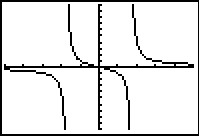
\includegraphics[width=2in]{./RationalsGraphics/Rationals02.jpg} \hspace{0.75in} & 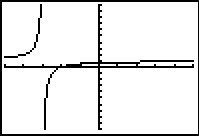
\includegraphics[width=2in]{./RationalsGraphics/Rationals03.jpg} \\

The graph of $y=f(x)$  \hspace{0.75in} & The graph of $y=g(x)$ \\


\end{tabular}
\end{center} 

\item  The domain of $h$ is all real numbers, since $x^2+9 = 0$ has no real solutions.  Accordingly, the graph of $y=h(x)$ is devoid of both vertical asymptotes and holes.

\item  Setting $x^2+4x+4 = 0$ gives us $x=-2$ as the only real number of concern.  Simplifying, we see  $r(x) = \frac{x^2-x-6}{x^2+4x+4} = \frac{(x-3)(x+2)}{(x+2)^2} = \frac{x-3}{x+2}$.  Since $x=-2$ continues to produce a $0$ in the denominator of the reduced function, we know $x=-2$ is a vertical asymptote to the graph.  The calculator bears this out, and, moreover, we see that as $x\rightarrow -2^{-}$, $r(x) \rightarrow \infty$ and as $x \rightarrow -2^{+}$, $r(x) \rightarrow -\infty$.


\begin{center}

\begin{tabular}{cc}

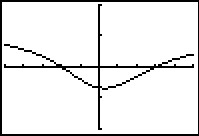
\includegraphics[width=2in]{./RationalsGraphics/Rationals04.jpg} \hspace{0.75in} & 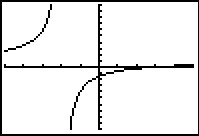
\includegraphics[width=2in]{./RationalsGraphics/Rationals05.jpg} \\

The graph of $y=h(x)$  \hspace{0.75in} & The graph of $y=r(x)$ \\


\end{tabular}
\end{center} 

\end{enumerate}
\qed
\end{ex}

Our next example gives us a physical interpretation of a vertical asymptote.  This type of model arises from a family of equations cheerily named `doomsday' equations.\footnote{These functions arise in Differential Equations.  The unfortunate name will make sense shortly.}  

\begin{ex}  A mathematical model for the population $P$, in thousands, of a certain species of bacteria, $t$ days after it is introduced to an environment is given by $P(t) = \frac{100}{(5-t)^{2}}$, $0 \leq t < 5$.


\begin{enumerate}

\item  Find and interpret $P(0)$.

\item  When will the population reach $100,\!000$?

\item  Determine the behavior of $P$ as $t \rightarrow 5^{-}$.  Interpret this result graphically and within the context of the problem. 

\end{enumerate}

{ \bf Solution.}  

\begin{enumerate}

\item  Substituting $t=0$ gives $P(0) = \frac{100}{(5-0)^2} = 4$, which means $4000$ bacteria are initially introduced into the environment.

\item  To find when the population reaches $100,\! 000$, we first need to remember that $P(t)$ is measured in \textit{thousands}.  In other words, $100,\! 000$ bacteria corresponds to $P(t) = 100$.  Substituting for $P(t)$ gives the equation  $\frac{100}{(5-t)^2} = 100$.  Clearing denominators and dividing by $100$ gives $(5-t)^2=1$, which, after extracting square roots, produces $t = 4$ or $t=6$.  Of these two solutions, only $t=4$ in in our domain, so this is the solution we keep.  Hence, it takes $4$ days for the population of bacteria to reach $100,\! 000$.

\item To determine the behavior of $P$ as $t \rightarrow 5^{-}$, we can make a table

\[\begin{array}{|r||c|}  \hline

  t & P(t)  \\ \hline
 4.9 & 10000  \\  \hline
 4.99 & 1000000  \\  \hline
 4.999 &  100000000  \\  \hline
  4.9999 & 10000000000  \\  \hline
  \end{array}\]

In other words, as $t \rightarrow 5^{-}$, $P(t) \rightarrow \infty$.  Graphically, the line $t=5$ is a vertical asymptote of the graph of $y=P(t)$.  Physically, this means that the population of bacteria is increasing without bound as we near 5 days, which cannot actually happen.  For this reason, $t=5$ is called the `doomsday' for this population. There is no way any environment can support infinitely many bacteria, so shortly before $t = 5$ the environment would collapse. \qed

\end{enumerate}

Now that we have thoroughly investigated vertical asymptotes, we can turn our attention to horizontal asymptotes.  The next theorem tells us when to expect horizontal asymptotes.

\smallskip
\colorbox{ResultColor}{\bbm

\begin{thm} \index{asymptote ! horizontal ! location of}\index{horizontal asymptote ! location of}\textbf{Location of Horizontal Asymptotes:}\label{hathm} Suppose $r$ is a rational function and $r(x) = \frac{p(x)}{q(x)}$, where $p$ and $q$ are polynomial functions with leading coefficients $a$ and $b$, respectively. 

\begin{itemize}

\item  If the degree of $p(x)$ is the same as the degree of $q(x)$, then $y=\frac{a}{b}$ is the\footnote{The use of the definite article will be justified momentarily.} horizontal asymptote of the graph of $y=r(x)$.

\item  If the degree of $p(x)$ is less than the degree of $q(x)$, then $y=0$ is the horizontal asymptote of the graph of $y=r(x)$.

\item  If the degree of $p(x)$ is greater than the degree of $q(x)$, then the graph of $y=r(x)$ has no horizontal asymptotes.


\end{itemize}
\end{thm}
\ebm}
\smallskip

\end{ex}

Like Theorem \ref{vavshole}, Theorem \ref{hathm} is proved using Calculus.  Nevertheless, we can understand the idea behind it using our example $f(x) = \frac{2x-1}{x+1}$.  If we interpret $f(x)$ as a division problem, $(2x-1) \div (x+1)$, we find that the quotient is $2$ with a remainder of $-3$.  Using what we know about polynomial division, specifically Theorem \ref{polydiv}, we get $2x-1 = 2(x+1) -3$.  Dividing both sides by $(x+1)$ gives   $\frac{2x-1}{x+1} = 2 - \frac{3}{x+1}$.  (You may remember this as the formula for $g(x)$ in Example \ref{ratfuncex}.)  As $x$ becomes unbounded in either direction, the quantity $\frac{3}{x+1}$ gets closer and closer to $0$ so that the values of $f(x)$ become closer and closer\footnote{As seen in the tables immediately preceding Definition \ref{va}.} to $2$. In symbols, as $x \rightarrow \pm \infty$, $f(x) \rightarrow 2$, and we have the result.\footnote{More specifically, as $x \rightarrow -\infty$, $f(x) \rightarrow 2^{+}$, and as $x \rightarrow \infty$, $f(x) \rightarrow 2^{-}$.}  Notice that the graph gets close to the same $y$ value as $x \rightarrow -\infty$ or $x \rightarrow \infty$.  This means that the graph can have only \underline{one} horizontal asymptote if it is going to have one at all.  Thus we were justified in using `the' in the previous theorem.

\smallskip

Alternatively, we can use what we know about end behavior of polynomials to help us understand this theorem.  From Theorem \ref{EBPolynomials}, we know the end behavior of a polynomial is determined by its leading term.  Applying this to the numerator and denominator of $f(x)$, we get that as $x \rightarrow \pm \infty$, $f(x) = \frac{2x-1}{x+1} \approx \frac{2x}{x} = 2$.  This last approach is useful in Calculus, and, indeed, is made rigorous there.  (Keep this in mind for the remainder of this paragraph.)  Applying this reasoning to the general case, suppose $r(x) = \frac{p(x)}{q(x)}$ where $a$ is the leading coefficient of $p(x)$ and $b$ is the leading coefficient of $q(x)$. As $x \rightarrow \pm \infty$, $r(x) \approx \frac{ax^n}{bx^m}$, where $n$ and $m$ are the degrees of $p(x)$ and $q(x)$, respectively.  If the degree of $p(x)$ and the degree of $q(x)$ are the same, then $n=m$ so that $r(x) \approx \frac{a}{b}$, which means $y=\frac{a}{b}$ is the horizontal asymptote in this case.  If the degree of $p(x)$ is less than the degree of $q(x)$, then $n < m$, so $m-n$ is a positive number, and hence, $r(x) \approx \frac{a}{bx^{m-n}} \rightarrow 0$ as $x \rightarrow \pm \infty$.  If the degree of $p(x)$ is greater than the degree of $q(x)$, then $n > m$, and hence $n-m$ is a positive number and $r(x) \approx \frac{ax^{n-m}}{ b}$, which becomes unbounded as $x \rightarrow \pm \infty$.  As we said before, if a rational function has a horizontal asymptote, then it will have only one.  (This is not true for other types of functions we shall see in later chapters.)
 
\begin{ex} \label{haexample} List the horizontal asymptotes, if any, of the graphs of the following functions.  Verify your answers using a graphing calculator, and describe the behavior of the graph near them using proper notation.

\begin{multicols}{3}

\begin{enumerate}

\item $f(x) = \dfrac{5x}{x^2+1}$  

\item  $g(x) = \dfrac{x^2-4}{x+1}$

\item  $h(x) = \dfrac{6x^3-3x+1}{5-2x^3}$

\end{enumerate}

\end{multicols}

{ \bf Solution.}

\begin{enumerate}

\item  The numerator of $f(x)$ is $5x$, which has degree $1$.  The denominator of $f(x)$ is $x^2+1$, which has degree $2$.  Applying Theorem \ref{hathm},  $y=0$ is the horizontal asymptote.  Sure enough, we see from the graph that as $x \rightarrow - \infty$, $f(x) \rightarrow 0^{-}$ and as $x \rightarrow \infty$, $f(x) \rightarrow 0^{+}$.

\item  The numerator of $g(x)$, $x^2-4$, has degree $2$, but the degree of the denominator, $x+1$, has degree $1$.  By Theorem \ref{hathm}, there is no horizontal asymptote.  From the graph, we see that the graph of $y=g(x)$ doesn't appear to level off to a constant value, so there is no horizontal asymptote.\footnote{Sit tight!  We'll revisit this function and its end behavior shortly.}

\item  The degrees of the numerator and denominator of $h(x)$ are both three, so Theorem \ref{hathm} tells us $y = \frac{6}{-2} = -3$ is the horizontal asymptote.  We see from the calculator's graph that as $x \rightarrow -\infty$, $h(x) \rightarrow -3^{+}$, and as $x \rightarrow \infty$, $h(x) \rightarrow -3^{-}$.

\begin{center}

\begin{tabular}{ccc}

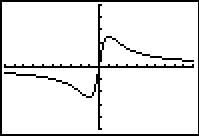
\includegraphics[width=1.75in]{./RationalsGraphics/Rationals06.jpg}  & 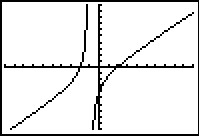
\includegraphics[width=1.75in]{./RationalsGraphics/Rationals07.jpg} & 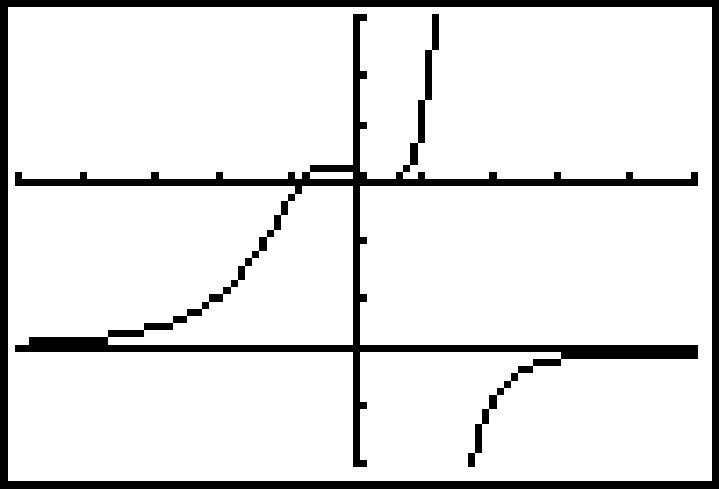
\includegraphics[width=1.75in]{./RationalsGraphics/Rationals08.jpg} \\

The graph of $y=f(x)$  & The graph of $y=g(x)$ & The graph of $y=h(x)$ \\


\end{tabular}
\end{center} 

\end{enumerate}

\vspace{-.25in} \qed

\end{ex}

Our next example of the section gives us a real-world application of a horizontal asymptote.\footnote{Though the population below is more accurately modeled with the functions in Chapter \ref{ExpLogs}, we approximate it (using Calculus, of course!) using a rational function.}

\begin{ex}  The number of students $N$ at local college who have had the flu $t$ months after the semester begins can be modeled by the formula $N(t) = 500 - \frac{450}{1+3t}$ for $t \geq 0$.

\begin{enumerate}

\item  Find and interpret $N(0)$.

\item  How long will it take until $300$ students will have had the flu?

\item  Determine the behavior of $N$ as $t \rightarrow \infty$.  Interpret this result graphically and within the context of the problem. 

\end{enumerate}

{ \bf Solution.}

\begin{enumerate}

\item  $N(0) = 500 - \frac{450}{1+3(0)} = 50$.  This means that at the beginning of the semester, $50$ students have had the flu.

\item  We set $N(t) = 300$ to get $500 - \frac{450}{1+3t} = 300$ and solve.  Isolating the fraction gives $\frac{450}{1+3t} = 200$.  Clearing denominators gives $450 = 200(1+3t)$.  Finally, we get $t = \frac{5}{12}$.  This means it will take $\frac{5}{12}$ months, or about 13 days, for $300$ students to have had the flu.

\item  To determine the behavior of $N$ as $t\rightarrow \infty$, we can use a table. 


\[\begin{array}{|r||c|}  \hline

  t & N(t)  \\ \hline
 10 & \approx 485.48  \\  \hline
 100& \approx 498.50  \\  \hline
 1000 &  \approx 499.85  \\  \hline
  10000 & \approx 499.98  \\  \hline
  \end{array}\]
  
The table suggests that as $t \rightarrow \infty$, $N(t) \rightarrow 500$. (More specifically, $500^{-}$.)  This means as time goes by, only a total of 500 students will have ever had the flu. \qed

\end{enumerate}

\end{ex}

We close this section with a discussion of the \textit{third} (and final!) kind of asymptote which can be associated with the graphs of rational functions. Let us return to the function $g(x) = \frac{x^2-4}{x+1}$ in Example \ref{haexample}. Performing long division,\footnote{See the remarks following Theorem \ref{hathm}.} we get $g(x) = \frac{x^2-4}{x+1} = x-1 - \frac{3}{x+1}$.  Since the term $\frac{3}{x+1} \rightarrow 0$ as $x \rightarrow \pm \infty$, it stands to reason that as $x$ becomes unbounded, the function values   $g(x) = x-1 - \frac{3}{x+1} \approx x-1$.  Geometrically, this means that the graph of $y=g(x)$ should resemble the line $y = x-1$ as $x \rightarrow \pm \infty$.  We see this play out both numerically and graphically below.

\begin{center}
\begin{tabular}{cc}

$\begin{array}{|r||c|c|}  \hline

  x & g(x) & x-1 \\ \hline
 -10 & \approx -10.6667 & -11 \\  \hline
 -100 & \approx -100.9697 & -101 \\  \hline 
 -1000 &  \approx -1000.9970&   -1001 \\ \hline 
  -10000 &  \approx -10000.9997 &  -10001 \\ \hline 
  \end{array} $ & \hspace{0.75in}

$\begin{array}{|r||c|c|}  \hline

  x & g(x) & x-1 \\ \hline
 10 & \approx 8.7273 &    9 \\\hline
 100 & \approx 98.9703 &   99 \\ \hline 
 1000 &  \approx 998.9970 &  999 \\ \hline 
  10000 &  \approx 9998.9997 &   9999 \\ \hline 
  \end{array} $ \\ 
  
  & \\
  
  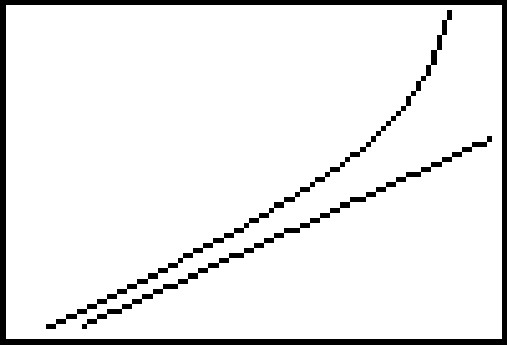
\includegraphics[width=2in]{./RationalsGraphics/SA01.jpg} & \hspace{0.75in}
  
  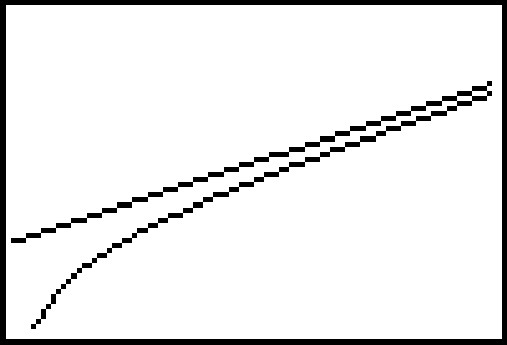
\includegraphics[width=2in]{./RationalsGraphics/SA02.jpg} \\
  
   $y= g(x)$ and $y=x-1$ & \hspace{0.75in} $y = g(x)$ and $y=x-1$ \\
    as $x \rightarrow -\infty$ & \hspace{0.75in} as $x \rightarrow \infty$ \\

\end{tabular}

\end{center}

The way we symbolize the relationship between the end behavior of $y=g(x)$ with that of the line $y=x-1$ is to write `as $x \rightarrow \pm \infty$, $g(x) \rightarrow x-1$.'  In this case, we say the line $y=x-1$ is a \index{asymptote ! slant (oblique)} \index{slant asymptote} \index{oblique asymptote} \textbf{slant asymptote}\footnote{Also called an `oblique' asymptote in some, ostensibly higher class (and more expensive), texts.}  to the graph of $y=g(x)$.  Informally, the graph of a rational function has a slant asymptote if, as $x \rightarrow \infty$ or as $x \rightarrow -\infty$, the graph resembles a non-horizontal, or `slanted' line.  Formally, we define a slant asymptote as follows.


\medskip


\colorbox{ResultColor}{\bbm

\begin{defn} \label{sa} The line $y = mx+b$ where $m \neq 0$  is called a \index{asymptote ! slant ! formal definition of}\index{slant asymptote ! formal definition of}\textbf{slant asymptote} of the graph of a function $y=f(x)$ if as $x \rightarrow -\infty$ or as $x \rightarrow \infty$, $f(x)  \rightarrow mx+b$.


\end{defn}
\ebm}

\medskip


A few remarks are in order.  First, note that the stipulation $m \neq 0$ in Definition \ref{sa} is what makes the `slant' asymptote `slanted' as opposed to the case when $m=0$ in which case we'd have a horizontal asymptote.  Secondly, while we have motivated what me mean intuitively by the notation `$f(x)  \rightarrow mx+b$,' like so many ideas in this section, the formal definition requires Calculus.  Another way to express this sentiment, however, is to rephrase `$f(x)  \rightarrow mx+b$' as `$f(x) - (mx+b) \rightarrow 0$.'  In other words, the graph of $y=f(x)$ has the \textit{slant} asymptote $y = mx+b$ if and only if the graph of $y = f(x) - (mx+b)$ has a \textit{horizontal} asymptote $y=0$.


Our next task is to determine the conditions under which the graph of a rational function has a slant asymptote, and if it does, how to find it.  In the case of $g(x) = \frac{x^2-4}{x+1}$, the degree of the numerator $x^2-4$ is $2$, which is \textit{exactly one more} than the degree if its denominator $x+1$ which is $1$.  This results in a \textit{linear} quotient polynomial, and it is this quotient polynomial which is the slant asymptote.  Generalizing this situation gives us the following theorem.\footnote{Once again, this theorem is brought to you courtesy of Theorem \ref{polydiv} and Calculus.}

\medskip

\colorbox{ResultColor}{\bbm

\begin{thm} \textbf{Determination of Slant Asymptotes:} \label{sathm} Suppose $r$ is a rational function and $r(x) = \frac{p(x)}{q(x)}$, where the degree of $p$ is \textit{exactly} one more than the degree of $q$.  Then the graph of $y=r(x)$ has \index{asymptote ! slant ! determination of}\index{slant asymptote ! determination of} the slant asymptote $y=L(x)$ where $L(x)$ is the quotient obtained by dividing $p(x)$ by $q(x)$.

\end{thm}
\ebm}

\medskip

In the same way that Theorem \ref{hathm} gives us an easy way to see if the graph of a rational function $r(x) = \frac{p(x)}{q(x)}$ has a horizontal asymptote by comparing the degrees of the numerator and denominator, Theorem \ref{sathm} gives us an easy way to check for slant asymptotes.  Unlike Theorem \ref{hathm}, which gives us a quick way to \textit{find} the horizontal asymptotes (if any exist), Theorem \ref{sathm} gives us no such `short-cut'.  If a slant asymptote exists, we have no recourse but to use long division to find it.\footnote{That's OK, though.  In the next section, we'll use long division to analyze end behavior and it's worth the effort!}  

\begin{ex} \label{saexample} Find the slant asymptotes of the graphs of the following functions if they exist.  Verify your answers using a graphing calculator and describe the behavior of the graph near them using proper notation.

\begin{multicols}{3}

\begin{enumerate}

\item  $f(x) = \dfrac{x^2-4x+2}{1-x}$  

\item  \label{sacancel} $g(x) = \dfrac{x^2-4}{x-2}$

\item  $h(x) = \dfrac{x^3+1}{x^2-4}$

\end{enumerate}

\end{multicols}


{\bf Solution.}

\begin{enumerate}

\item  The degree of the numerator is $2$ and the degree of the denominator is $1$, so Theorem \ref{sathm} guarantees us a slant asymptote.  To find it, we divide $1-x = -x+1$ into $x^2-4x+2$ and get a quotient of $-x+3$, so our slant asymptote is $y=-x+3$.  We confirm this graphically, and we see that as $x \rightarrow -\infty$, the graph of $y=f(x)$ approaches the asymptote from below, and as $x \rightarrow \infty$, the graph of $y=f(x)$ approaches the asymptote from above.\footnote{Note that we are purposefully avoiding notation like `as $x\rightarrow \infty$, $f(x) \rightarrow (-x+3)^{+}$.  While it is possible to define these notions formally with Calculus, it is not standard to do so.  Besides, with the introduction of the symbol `\textinterrobang' in the next section, the authors feel we are in enough trouble already.}

\item  As with the previous example, the degree of the numerator $g(x) = \frac{x^2-4}{x-2}$ is $2$ and the degree of the denominator is $1$, so Theorem \ref{sathm} applies.  In this case, 

\[ g(x) = \frac{x^2-4}{x-2} = \frac{(x+2)(x-2)}{(x-2)} = \frac{(x+2) \cancel{(x-2)}}{\cancelto{1}{(x-2)}} = x+2, \quad x \neq 2\]

so we have that the slant asymptote $y=x+2$ is identical to the graph of $y=g(x)$ except at $x=2$ (where the latter has a `hole' at $(2,4)$.)  The calculator supports this claim.\footnote{While the word `asymptote' has the connotation of `approaching but not equaling,' Definitions \ref{ha} and \ref{sa} invite the same kind of pathologies we saw with Definitions \ref{maxmindefn} in Section \ref{GraphsofFunctions}.}

\item   For $h(x) = \frac{x^3+1}{x^2-4}$, the degree of the numerator is $3$ and the degree of the denominator is $2$ so again, we are guaranteed the existence of a slant asymptote.  The long division $\left(x^3+1 \right) \div \left(x^2-4\right)$ gives a quotient of just $x$, so our slant asymptote is the line $y=x$.  The calculator confirms this, and we find that as $x \rightarrow -\infty$, the graph of $y=h(x)$ approaches the asymptote from below, and as $x \rightarrow \infty$, the graph of $y=h(x)$ approaches the asymptote from above. 

\begin{center}

\begin{tabular}{ccc}

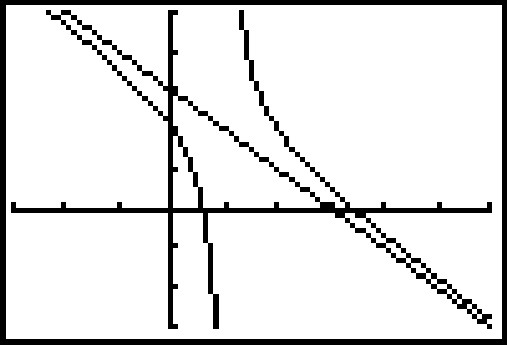
\includegraphics[width=1.75in]{./RationalsGraphics/SAEX01.jpg}  & 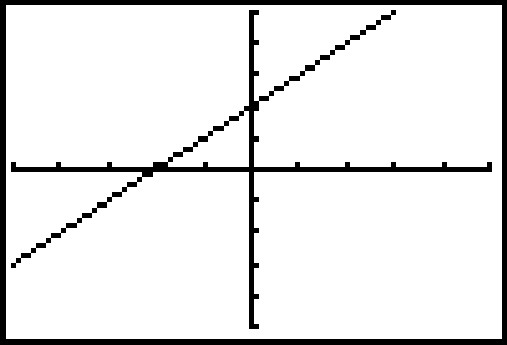
\includegraphics[width=1.75in]{./RationalsGraphics/SAEX02.jpg} & 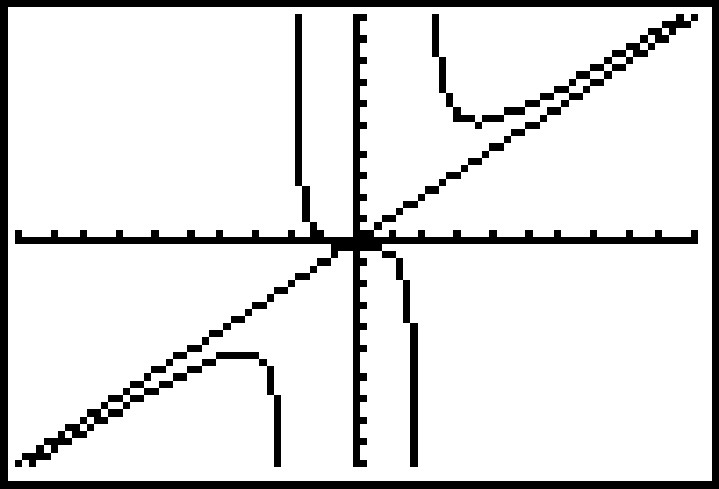
\includegraphics[width=1.75in]{./RationalsGraphics/SAEX03.jpg} \\

The graph of $y=f(x)$  & The graph of $y=g(x)$ & The graph of $y=h(x)$ \\


\end{tabular}
\end{center} 


\qed

\end{enumerate}

\end{ex}



The reader may be a bit disappointed with the authors at this point owing to the fact that in Examples \ref{vavsholeexample}, \ref{haexample}, and \ref{saexample}, we used the \textit{calculator} to determine function behavior near asymptotes.  We rectify that in the next section where we, in excruciating detail, demonstrate the usefulness of `number sense' to reveal this behavior analytically.  
\newpage

\subsection{Exercises}

In Exercises \ref{alltheasympfirst} - \ref{alltheasymplast}, for the given rational function $f$:

\begin{itemize}

\item Find the domain of $f$.
\item Identify any vertical asymptotes of the graph of $y = f(x)$.
\item Identify any holes in the graph.
\item Find the horizontal asymptote, if it exists.
\item Find the slant asymptote, if it exists.
\item Graph the function using a graphing utility and describe the behavior near the asymptotes.

\end{itemize}

\begin{multicols}{3}
\begin{enumerate}

\item $f(x) = \dfrac{x}{3x - 6}$ \label{alltheasympfirst}
\item $f(x) = \dfrac{3 + 7x}{5 - 2x}$
\item $f(x) = \dfrac{x}{x^{2} + x - 12}$

\setcounter{HW}{\value{enumi}}
\end{enumerate}
\end{multicols}

\begin{multicols}{3}
\begin{enumerate}
\setcounter{enumi}{\value{HW}}

\item $f(x) = \dfrac{x}{x^{2} + 1}$
\item $f(x) = \dfrac{x + 7}{(x + 3)^{2}}$
\item $f(x) = \dfrac{x^{3} + 1}{x^{2} - 1}$

\setcounter{HW}{\value{enumi}}
\end{enumerate}
\end{multicols}

\begin{multicols}{3}
\begin{enumerate}
\setcounter{enumi}{\value{HW}}

\item $f(x) = \dfrac{4x}{x^2+4}$
\item $f(x) = \dfrac{4x}{x^2-4}$
\item $f(x) = \dfrac{x^2-x-12}{x^2+x-6}$

\setcounter{HW}{\value{enumi}}
\end{enumerate}
\end{multicols}

\begin{multicols}{3}
\begin{enumerate}
\setcounter{enumi}{\value{HW}}

\item $f(x) = \dfrac{3x^2-5x-2}{x^2-9}$
\item $f(x) = \dfrac{x^3+2x^2+x}{x^2-x-2}$
\item $f(x) = \dfrac{x^{3} - 3x + 1}{x^{2} + 1}$

\setcounter{HW}{\value{enumi}}
\end{enumerate}
\end{multicols}

\begin{multicols}{3}
\begin{enumerate}
\setcounter{enumi}{\value{HW}}

\item $f(x) = \dfrac{2x^{2} + 5x - 3}{3x + 2}$
\item $f(x) = \dfrac{-x^{3} + 4x}{x^{2} - 9}$
\item \small $f(x) = \dfrac{-5x^{4} - 3x^{3} + x^{2} - 10}{x^{3} - 3x^{2} + 3x - 1}$ \normalsize 

\setcounter{HW}{\value{enumi}}
\end{enumerate}
\end{multicols}


\begin{multicols}{3}
\begin{enumerate}
\setcounter{enumi}{\value{HW}}

\item $f(x) = \dfrac{x^3}{1-x}$
\item $f(x) = \dfrac{18-2x^2}{x^2-9}$
\item $f(x) = \dfrac{x^3-4x^2-4x-5}{x^2+x+1}$ \label{alltheasymplast}


\setcounter{HW}{\value{enumi}}
\end{enumerate}
\end{multicols}

\begin{enumerate}
\setcounter{enumi}{\value{HW}}

\item The cost $C$ in dollars to remove $p$\% of the invasive species of Ippizuti fish from Sasquatch Pond is given by \[C(p) = \frac{1770p}{100 - p}, \quad 0 \leq p < 100 \]

\begin{enumerate}

\item Find and interpret $C(25)$ and $C(95)$.
\item What does the vertical asymptote at $x = 100$ mean within the context of the problem?  
\item What percentage of the Ippizuti fish can you remove for  \$40000?

\end{enumerate}


\item In Exercise \ref{Sasquatchfunc1} in Section \ref{FunctionNotation}, the population of Sasquatch in Portage County was modeled by the function \[P(t) = \frac{150t}{t + 15},\] where $t = 0$ represents the year 1803.  Find the horizontal asymptote of the graph of $y = P(t)$ and explain what it means.

\item  Recall from Example \ref{costrevenueprofitex1} that the cost $C$ (in dollars) to make $x$ dOpi media players is $C(x) = 100x+2000$, $x \geq 0$.  

\begin{enumerate}

\item  Find a formula for the average cost $\overline{C}(x)$. Recall:  $\overline{C}(x) = \frac{C(x)}{x}$.

\item  Find and interpret $\overline{C}(1)$ and $\overline{C}(100)$.

\item  How many dOpis need to be produced so that the average cost per dOpi is $\$ 200$?

\item  Interpret the behavior of $\overline{C}(x)$ as $x \rightarrow 0^{+}$.  (HINT:  You may want to find the fixed cost $C(0)$ to help in your interpretation.)

\item  Interpret the behavior of $\overline{C}(x)$ as $x \rightarrow \infty$.  (HINT:  You may want to find the variable cost (defined in Example \ref{PortaBoyCost} in Section \ref{LinearFunctions}) to help in your interpretation.)


\end{enumerate}

\item In Exercise \ref{circuitexercisepoly} in Section \ref{GraphsofPolynomials}, we fit a few polynomial models to the following electric circuit data. (The circuit was built with a variable resistor.  For each of the following resistance values (measured in kilo-ohms, $k \Omega$),  the corresponding power to the load (measured in milliwatts, $mW$) is given in the table below.)\footnote{The authors wish to thank Don Anthan and Ken White of Lakeland Community College for devising this problem and generating the accompanying data set.}


\smallskip

\noindent \begin{tabular}{|l|r|r|r|r|r|r|} \hline
Resistance: ($k \Omega$) & 1.012 & 2.199 & 3.275 & 4.676 & 6.805 & 9.975 \\ \hline
Power: ($mW$) & 1.063 & 1.496 & 1.610 & 1.613 & 1.505 & 1.314 \\ \hline
\end{tabular}

\smallskip

\noindent Using some fundamental laws of circuit analysis mixed with a healthy dose of algebra, we can derive the actual formula relating power to resistance.  For this circuit, it is $P(x) = \frac{25x}{(x + 3.9)^2}$, where $x$ is the resistance value, $x \geq 0$.

\begin{enumerate}

\item Graph the data along with the function $y = P(x)$ on your calculator.

\item Use your calculator to approximate the maximum power that can be delivered to the load.  What is the corresponding resistance value?

\item Find and interpret the end behavior of $P(x)$ as $x \rightarrow \infty$.

\end{enumerate}

\item \index{Learning Curve Equation} \index{Thurstone, Louis Leon} In his now famous 1919 dissertation \underline{The Learning Curve Equation}, Louis Leon Thurstone presents a rational function which models the number of words a person can type in four minutes as a function of the number of pages of practice one has completed.  (This paper, which is now in the public domain and can be found  \href{http://books.google.com/books?id=pb5BAAAAIAAJ&dq=Louis+Leon+Thurstone&printsec=frontcover&source=an&hl=en&ei=Ev_bSaeKGInEMbmM9OQN&sa=X&oi=book_result&ct=result&resnum=6#PPP1,M1}{\underline{here}}, is from a bygone era when students at business schools took typing classes on manual typewriters.)  Using his original notation and original language, we have $Y = \frac{L(X + P)}{(X + P) + R}$ where $L$ is the predicted practice limit in terms of speed units, $X$ is pages written, $Y$ is writing speed in terms of words in four minutes, $P$ is equivalent previous practice in terms of pages and $R$ is the rate of learning. In Figure 5 of the paper, he graphs a scatter plot and the curve $Y = \frac{216(X + 19)}{X + 148}$.  Discuss this equation with your classmates.  How would you update the notation?  Explain what the horizontal asymptote of the graph means.  You should take some time to look at the original paper. Skip over the computations you don't understand yet and try to get a sense of the time and place in which the study was conducted.

\end{enumerate}

\newpage

\subsection{Answers}

\begin{multicols}{2}
\begin{enumerate} 

\item $f(x) = \dfrac{x}{3x - 6}$ \vphantom{$\dfrac{7x}{7x}$}\\ 
Domain: $(-\infty, 2) \cup (2, \infty)$\\
Vertical asymptote: $x = 2$\\
As $x \rightarrow 2^{-}, f(x) \rightarrow -\infty$\\
As $x \rightarrow 2^{+}, f(x) \rightarrow \infty$\\
No holes in the graph\\
Horizontal asymptote: $y = \frac{1}{3}$ \\
As $x \rightarrow -\infty, f(x) \rightarrow \frac{1}{3}^{-}$\\
As $x \rightarrow \infty, f(x) \rightarrow \frac{1}{3}^{+}$\\

\vfill

\columnbreak

\item $f(x) = \dfrac{3 + 7x}{5 - 2x}$\\
Domain: $(-\infty, \frac{5}{2}) \cup (\frac{5}{2}, \infty)$\\
Vertical asymptote: $x = \frac{5}{2}$\\
As $x \rightarrow \frac{5}{2}^{-}, f(x) \rightarrow \infty$\\
As $x \rightarrow \frac{5}{2}^{+}, f(x) \rightarrow -\infty$\\
No holes in the graph\\
Horizontal asymptote: $y = -\frac{7}{2}$ \\
As $x \rightarrow -\infty, f(x) \rightarrow -\frac{7}{2}^{+}$\\
As $x \rightarrow \infty, f(x) \rightarrow -\frac{7}{2}^{-}$\\

\setcounter{HW}{\value{enumi}}
\end{enumerate}
\end{multicols}

\begin{multicols}{2}
\begin{enumerate}
\setcounter{enumi}{\value{HW}}

\item $f(x) = \dfrac{x}{x^{2} + x - 12} = \dfrac{x}{(x + 4)(x - 3)}$\\
Domain: $(-\infty, -4) \cup (-4, 3) \cup (3, \infty)$\\
Vertical asymptotes: $x = -4, x = 3$\\
As $x \rightarrow -4^{-}, f(x) \rightarrow -\infty$\\
As $x \rightarrow -4^{+}, f(x) \rightarrow \infty$\\
As $x \rightarrow 3^{-}, f(x) \rightarrow -\infty$\\
As $x \rightarrow 3^{+}, f(x) \rightarrow \infty$\\
No holes in the graph\\
Horizontal asymptote: $y = 0$ \\
As $x \rightarrow -\infty, f(x) \rightarrow 0^{-}$\\
As $x \rightarrow \infty, f(x) \rightarrow 0^{+}$\\

\vfill

\columnbreak


\item $f(x) = \dfrac{x}{x^{2} + 1}$\\
Domain: $(-\infty, \infty)$\\
No vertical asymptotes\\
No holes in the graph\\
Horizontal asymptote: $y = 0$ \\
As $x \rightarrow -\infty, f(x) \rightarrow 0^{-}$\\
As $x \rightarrow \infty, f(x) \rightarrow 0^{+}$\\

\setcounter{HW}{\value{enumi}}
\end{enumerate}
\end{multicols}

\begin{multicols}{2}
\begin{enumerate}
\setcounter{enumi}{\value{HW}}

\item $f(x) = \dfrac{x + 7}{(x + 3)^{2}}$ \vphantom{$\dfrac{x^{3}}{x^{2}}$}\\
Domain: $(-\infty, -3) \cup (-3, \infty)$\\
Vertical asymptote: $x = -3$\\
As $x \rightarrow -3^{-}, f(x) \rightarrow \infty$\\
As $x \rightarrow -3^{+}, f(x) \rightarrow \infty$\\
No holes in the graph\\
Horizontal asymptote: $y = 0$ \\
\footnote{This is hard to see on the calculator, but trust me, the graph is below the $x$-axis to the left of $x = -7$.}As $x \rightarrow -\infty, f(x) \rightarrow 0^{-}$\\
As $x \rightarrow \infty, f(x) \rightarrow 0^{+}$\\

\vfill

\columnbreak

\item $f(x) = \dfrac{x^{3} + 1}{x^{2} - 1} = \dfrac{x^{2} - x+ 1}{x-1}$\\
Domain: $(-\infty, -1) \cup (-1, 1) \cup (1, \infty)$\\
Vertical asymptote: $x = 1$\\
As $x \rightarrow 1^{-}, f(x) \rightarrow -\infty$\\
As $x \rightarrow 1^{+}, f(x) \rightarrow \infty$\\
Hole at $(-1, -\frac{3}{2})$\\
Slant asymptote: $y=x$  \\
As $x \rightarrow -\infty$, the graph is below $y=x$\\
As $x \rightarrow \infty$, the graph is above $y=x$\\

\setcounter{HW}{\value{enumi}}
\end{enumerate}
\end{multicols}

\begin{multicols}{2}
\begin{enumerate}
\setcounter{enumi}{\value{HW}}

\item $f(x) = \dfrac{4x}{x^{2} + 4}$\\
Domain: $(-\infty,  \infty)$\\
No vertical asymptotes \\
No holes in the graph\\
Horizontal asymptote: $y = 0$ \\
As $x \rightarrow -\infty, f(x) \rightarrow 0^{-}$\\
As $x \rightarrow \infty, f(x) \rightarrow 0^{+}$\\


\vfill

\columnbreak

\item $f(x) = \dfrac{4x}{x^{2} -4} = \dfrac{4x}{(x + 2)(x - 2)}$\\
Domain: $(-\infty, -2) \cup (-2, 2) \cup (2, \infty)$\\
Vertical asymptotes: $x = -2, x = 2$\\
As $x \rightarrow -2^{-}, f(x) \rightarrow -\infty$\\
As $x \rightarrow -2^{+}, f(x) \rightarrow \infty$\\
As $x \rightarrow 2^{-}, f(x) \rightarrow -\infty$\\
As $x \rightarrow 2^{+}, f(x) \rightarrow \infty$\\
No holes in the graph\\
Horizontal asymptote: $y = 0$ \\
As $x \rightarrow -\infty, f(x) \rightarrow 0^{-}$\\
As $x \rightarrow \infty, f(x) \rightarrow 0^{+}$\\

\setcounter{HW}{\value{enumi}}
\end{enumerate}
\end{multicols}

\begin{multicols}{2}
\begin{enumerate}
\setcounter{enumi}{\value{HW}}

\item $f(x) = \dfrac{x^2-x-12}{x^{2} +x - 6} = \dfrac{x-4}{x - 2}$\\
Domain: $(-\infty, -3) \cup (-3, 2) \cup (2, \infty)$\\
Vertical asymptote: $x = 2$\\
As $x \rightarrow 2^{-}, f(x) \rightarrow \infty$\\
As $x \rightarrow 2^{+}, f(x) \rightarrow -\infty$\\
Hole at $\left(-3, \frac{7}{5} \right)$ \\
Horizontal asymptote: $y = 1$ \\
As $x \rightarrow -\infty, f(x) \rightarrow 1^{+}$\\
As $x \rightarrow \infty, f(x) \rightarrow 1^{-}$\\


\vfill

\columnbreak

\item $f(x) = \dfrac{3x^2-5x-2}{x^{2} -9} = \dfrac{(3x+1)(x-2)}{(x + 3)(x - 3)}$\\
Domain: $(-\infty, -3) \cup (-3, 3) \cup (3, \infty)$\\
Vertical asymptotes: $x = -3, x = 3$\\
As $x \rightarrow -3^{-}, f(x) \rightarrow \infty$\\
As $x \rightarrow -3^{+}, f(x) \rightarrow -\infty$\\
As $x \rightarrow 3^{-}, f(x) \rightarrow -\infty$\\
As $x \rightarrow 3^{+}, f(x) \rightarrow \infty$\\
No holes in the graph\\
Horizontal asymptote: $y = 3$ \\
As $x \rightarrow -\infty, f(x) \rightarrow 3^{+}$\\
As $x \rightarrow \infty, f(x) \rightarrow 3^{-}$\\

\setcounter{HW}{\value{enumi}}
\end{enumerate}
\end{multicols}

\begin{multicols}{2}
\begin{enumerate}
\setcounter{enumi}{\value{HW}}


\item $f(x) = \dfrac{x^3+2x^2+x}{x^{2} -x-2} = \dfrac{x(x+1)}{x - 2}$\\
Domain: $(-\infty, -1) \cup (-1, 2) \cup (2, \infty)$\\
Vertical asymptote: $x = 2$\\
As $x \rightarrow 2^{-}, f(x) \rightarrow -\infty$\\
As $x \rightarrow 2^{+}, f(x) \rightarrow \infty$\\
Hole at $(-1,0)$ \\
Slant asymptote: $y=x+3$ \\
As $x \rightarrow -\infty$, the graph is below $y=x+3$\\
As $x \rightarrow \infty$, the graph is above $y=x+3$\\

\vfill

\columnbreak

\item $f(x) = \dfrac{x^3-3x+1}{x^2+1}$\\
Domain: $(-\infty, \infty)$\\
No vertical asymptotes \\
No holes in the graph \\
Slant asymptote: $y=x$ \\
As $x \rightarrow -\infty$, the graph is above $y=x$ \\
As $x \rightarrow \infty$, the graph is below $y=x$  \\


\setcounter{HW}{\value{enumi}}
\end{enumerate}
\end{multicols}

\newpage

\begin{multicols}{2}
\begin{enumerate}
\setcounter{enumi}{\value{HW}}

\item $f(x) = \dfrac{2x^{2} + 5x - 3}{3x + 2}$\\
Domain: $\left(-\infty, -\frac{2}{3}\right) \cup \left(-\frac{2}{3}, \infty\right)$\\
Vertical asymptote: $x = -\frac{2}{3}$\\
As $x \rightarrow -\frac{2}{3}^{-}, f(x) \rightarrow \infty$\\
As $x \rightarrow -\frac{2}{3}^{+}, f(x) \rightarrow -\infty$\\
No holes in the graph \\
Slant asymptote:  $y = \frac{2}{3}x + \frac{11}{9}$ \\
As $x \rightarrow  -\infty$, the graph is above \small $y = \frac{2}{3}x + \frac{11}{9}$\\
\normalsize As $x \rightarrow \infty$, the graph is below \small $y = \frac{2}{3}x + \frac{11}{9}$ \normalsize \\

\vfill

\columnbreak

\item $f(x) = \dfrac{-x^{3} + 4x}{x^{2} - 9} = \dfrac{-x^{3} + 4x}{(x-3)(x+3)} $\\
Domain: $(-\infty, -3) \cup (-3, 3) \cup (3, \infty)$\\
Vertical asymptotes: $x = -3$, $x=3$\\
As $x \rightarrow -3^{-}, f(x) \rightarrow \infty$\\
As $x \rightarrow -3^{+}, f(x) \rightarrow -\infty$\\
As $x \rightarrow 3^{-}, f(x) \rightarrow \infty$\\
As $x \rightarrow 3^{+}, f(x) \rightarrow -\infty$\\
No holes in the graph \\
Slant asymptote: $y=-x$ \\
As $x \rightarrow -\infty$, the graph is above $y=-x$\\
As $x \rightarrow \infty$, the graph is below $y=-x$\\


\setcounter{HW}{\value{enumi}}
\end{enumerate}
\end{multicols}

\begin{multicols}{2}
\begin{enumerate}
\setcounter{enumi}{\value{HW}}

\item \small $f(x) = \dfrac{-5x^{4} - 3x^{3} + x^{2} - 10}{x^{3} - 3x^{2} + 3x - 1} \\ \phantom{f(x)} = \dfrac{-5x^{4} - 3x^{3} + x^{2} - 10}{(x-1)^3} $ \normalsize \\
Domain: $(-\infty, 1) \cup (1, \infty)$\\
Vertical asymptotes: $x = 1$\\
As $x \rightarrow 1^{-}, f(x) \rightarrow \infty$\\
As $x \rightarrow 1^{+}, f(x) \rightarrow -\infty$\\
No holes in the graph \\
Slant asymptote: $y=-5x-18$ \\
 \small  As $x \rightarrow -\infty$, the graph is above $y=-5x-18$ \normalsize\\
 \small  As $x \rightarrow \infty$, the graph is below $y=-5x-18$ \normalsize \\
 
 \vfill
 
 \columnbreak

\item $f(x) = \dfrac{x^3}{1-x}$\\
Domain: $(-\infty, 1) \cup (1, \infty)$\\
Vertical asymptote: $x=1$\\
As $x \rightarrow 1^{-}, f(x) \rightarrow \infty$\\
As $x \rightarrow 1^{+}, f(x) \rightarrow -\infty$\\
No holes in the graph \\
No horizontal or slant asymptote \\
As $x \rightarrow -\infty$, $f(x) \rightarrow -\infty$\\
As $x \rightarrow \infty$, $f(x) \rightarrow -\infty$\\


\setcounter{HW}{\value{enumi}}
\end{enumerate}
\end{multicols}

\begin{multicols}{2}
\begin{enumerate}
\setcounter{enumi}{\value{HW}}

\item $f(x) = \dfrac{18-2x^2}{x^2-9} = -2$\\
Domain: $(-\infty, -3) \cup (-3,3) \cup (3, \infty)$\\
No vertical asymptotes \\
Holes in the graph at $(-3,-2)$ and $(3,-2)$ \\
Horizontal asymptote $y = -2$ \\
As $x \rightarrow \pm \infty$, $f(x) = -2$ \\

\vfill
\columnbreak

\item $f(x) = \dfrac{x^3-4x^2-4x-5}{x^2+x+1} = x-5$\\
Domain: $(-\infty, \infty)$\\
No vertical asymptotes \\
No holes in the graph \\
Slant asymptote:  $y = x-5$ \\
$f(x) = x-5$ everywhere. \\


\setcounter{HW}{\value{enumi}}
\end{enumerate}
\end{multicols}

\begin{enumerate}
\setcounter{enumi}{\value{HW}}

\item \begin{enumerate}

\item $C(25) = 590$ means it costs \$590 to remove 25\% of the fish and and $C(95)= 33630$ means it would cost \$33630 to remove 95\% of the fish from the pond.
\item The vertical asymptote at $x = 100$ means that as we try to remove 100\% of the fish from the pond, the cost increases without bound; i.e., it's impossible to remove all of the fish.  
\item For \$40000 you could remove about 95.76\% of the fish.

\end{enumerate}


\item The horizontal asymptote of the graph of $P(t) = \frac{150t}{t + 15}$ is $y = 150$ and it means that the model predicts the population of Sasquatch in Portage County will never exceed 150.

\item  \begin{enumerate}

\item $\overline{C}(x) = \frac{100x+2000}{x}$, $x > 0$.

\item  $\overline{C}(1) = 2100$ and $\overline{C}(100) = 120$. When just $1$ dOpi is produced, the cost per dOpi is $\$2100$, but when $100$ dOpis are produced, the cost per dOpi is $\$120$.  

\item  $\overline{C}(x) = 200$ when $x = 20$.  So to get the cost per dOpi to $\$200$, $20$ dOpis need to be produced.

\item  As $x \rightarrow 0^{+}$, $\overline{C}(x) \rightarrow \infty$.  This means that as fewer and fewer dOpis are produced, the cost per dOpi becomes unbounded.  In this situation, there is a fixed cost of $\$2000$ ($C(0) = 2000$), we are trying to spread that $\$2000$ over fewer and fewer dOpis.

\item   As $x \rightarrow \infty$,  $\overline{C}(x) \rightarrow 100^{+}$.  This means that as more and more dOpis are produced, the cost per dOpi approaches $\$100$, but is always a little more than $\$100$.  Since $\$100$ is the variable cost per dOpi ($C(x) = \underline{100}x+2000$), it means that no matter how many dOpis are produced, the average cost per dOpi will always be a bit higher than the variable cost to produce a dOpi.  As before, we can attribute this to the $\$2000$ fixed cost, which factors into the average cost per dOpi no matter how many dOpis are produced.


\end{enumerate}

\item \begin{enumerate}

\item $~$

\centerline{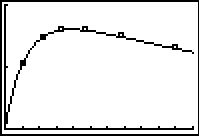
\includegraphics[width=2in]{./RationalsGraphics/CIRCRAT.jpg}}

\item The maximum power is approximately $1.603 \; mW$ which corresponds to $3.9 \; k\Omega$.

\item As $x \rightarrow \infty, \; P(x) \rightarrow 0^{+}$ which means as the resistance increases without bound, the power diminishes to zero.

\end{enumerate}

\end{enumerate}

\closegraphsfile

\newpage

\section{Graphs of Rational Functions}

\mfpicnumber{1}
\opengraphsfile{RationalGraphs}

\setcounter{footnote}{0}

\label{RationalGraphs}

In this section, we take a closer look at graphing rational functions.  In Section \ref{IntroRational}, we learned that the graphs of rational functions may have holes in them and could have vertical, horizontal and slant asymptotes.  Theorems \ref{vavshole}, \ref{hathm} and \ref{sathm} tell us exactly when and where these behaviors will occur, and if we combine these results with what we already know about graphing functions, we will quickly be able to generate reasonable graphs of rational functions.  

\smallskip

One of the standard tools we will use is the sign diagram which was first introduced in Section \ref{Inequalities}, and then revisited in Section \ref{GraphsofPolynomials}.  In those sections, we operated under the belief that a function couldn't change its sign without its graph crossing through the $x$-axis.  The major theorem we used to justify this belief was the Intermediate Value Theorem, Theorem \ref{IVT}.   It turns out the Intermediate Value Theorem applies to all \textit{continuous} functions,\footnote{Recall that, for our purposes, this means the graphs are devoid of any breaks, jumps or holes} not just polynomials. Although rational functions are continuous on their domains,\footnote{Another result from Calculus.} Theorem \ref{vavshole} tells us that vertical asymptotes and holes occur at the values excluded from their domains.  In other words, rational functions aren't continuous at these excluded values which leaves open the possibility that the function could change sign \textit{without} crossing through the $x$-axis.  Consider the graph of $y=h(x)$ from Example \ref{ratfuncex}, recorded below for convenience.  We have added its $x$-intercept at $\left(\frac{1}{2},0\right)$ for the discussion that follows. Suppose we wish to construct a sign diagram for $h(x)$.    Recall that the intervals where $h(x)>0$, or $(+)$, correspond to the $x$-values where the graph of $y=h(x)$ is \textit{above} the $x$-axis; the intervals on which $h(x) < 0$, or $(-)$ correspond to where the graph is \textit{below} the $x$-axis.  

\smallskip

\begin{tabular}{m{1in}m{2.5in}m{2in}}

&

\begin{mfpic}[15]{-5}{5}{-7}{9}
\arrow \reverse \arrow \function{-5,-1.5,0.1}{(2*x-1)/(x+1)}
\arrow \reverse \arrow  \function{-0.63,5,0.1}{(2*x-1)/(x+1)}
\gclear \circle{(1,0.5),0.1}
\circle{(1,0.5),0.1}
\point[3pt]{(0.5,0)}
\dashed \polyline{(-5,2), (5,2)}
\dashed \polyline{(-1,-6), (-1,8)}
\tlabel[cc](5,-0.5){\scriptsize $x$}
\tlabel[cc](0.5,9){\scriptsize $y$}
\tlabel[cc](0.5,-0.6){\scriptsize $\frac{1}{2}$}
\axes
\xmarks{-4 step 1 until 4}
\ymarks{-6 step 1 until 8}
\tiny
\tlpointsep{4pt}
\axislabels {x}{ {$-4 \hspace{7pt}$} -4, {$-3\hspace{7pt}$} -3, {$-2\hspace{7pt}$} -2,  {$1$} 1, {$2$} 2, {$3$} 3, {$4$} 4}
\axislabels {y}{ {$\hspace{1in} -1$} -1, {$-2$} -2, {$-3$} -3, {$-4$} -4, {$-5$} -5, {$-6$} -6,  {$1$} 1, {$3$} 3, {$4$} 4, {$5$} 5, {$6$} 6, {$7$} 7, {$8$} 8}
\normalsize
\end{mfpic}

&

\begin{mfpic}[10]{-6.5}{6.5}{-2}{2}
\arrow \reverse \arrow \polyline{(-6.5,0),(6.5,0)}
\xmarks{-3,0,3}
\tlpointsep{6pt}
\axislabels {x}{{$-1$} -3, {$\frac{1}{2}$} 0, {$1$} 3 }
\tlabel[cc](-5,1){$(+)$}
\tlabel[cc](-3,1){\textinterrobang}
\tlabel[cc](-1.5,1){$(-)$}
\tlabel[cc](0,1){$0$}
\tlabel[cc](1.5,1){$(+)$}
\tlabel[cc](3,1){\textinterrobang}
\tlabel[cc](5,1){$(+)$}
\end{mfpic} 

\end{tabular}

\enlargethispage{.25in}
\vspace{-.1in}

As we examine the graph of $y=h(x)$, reading from left to right, we note that from $(-\infty,-1)$, the graph is above the $x$-axis, so $h(x)$ is $(+)$ there.  At $x=-1$, we have a vertical asymptote, at which point the graph `jumps' across the $x$-axis.  On the interval $\left(-1,\frac{1}{2}\right)$, the graph is below the $x$-axis, so $h(x)$ is $(-)$ there.  The graph crosses through the $x$-axis at $\left(\frac{1}{2},0\right)$ and remains above the $x$-axis until $x=1$, where we have a `hole' in the graph.  Since $h(1)$ is undefined, there is no sign here.  So we have $h(x)$ as $(+)$ on the interval $\left(\frac{1}{2}, 1\right)$.  Continuing, we see that on $(1, \infty)$, the graph of $y=h(x)$ is above the $x$-axis, so we mark $(+)$ there.  To construct a sign diagram from this information, we not only need to denote the zero of $h$, but also the places not in the domain of $h$.  As is our custom, we write `$0$' above $\frac{1}{2}$ on the sign diagram to remind us that it is a zero of $h$.  We need a different notation for $-1$ and $1$, and we have chosen to use `\textinterrobang' - a nonstandard symbol called the \href{http://en.wikipedia.org/wiki/Interrobang}{\underline{interrobang}}.  \index{interrobang} We use this symbol to convey a sense of surprise, caution and wonderment - an appropriate attitude to take when approaching these points.   The moral of the story is that when constructing sign diagrams for rational functions, we include the zeros as well as the values excluded from the domain.

\medskip

\phantomsection
\label{rationalsigndiagram}

\colorbox{ResultColor}{\bbm

\centerline{\textbf{Steps for Constructing a Sign Diagram for a  Rational Function}} 

\medskip

\hspace{.17in} Suppose $r$ is a rational function. \index{sign diagram ! rational function}

\begin{enumerate}

\item  Place any values excluded from the domain of  $r$ on the number line with an `\textinterrobang' above them.

\item  Find the zeros of $r$ and place them on the number line with the number $0$ above them.

\item  Choose a test value in each of the intervals determined in steps 1 and 2.

\item  Determine the sign of $r(x)$ for each test value in step 3, and write that sign above the corresponding interval.

\end{enumerate}

\ebm}

\medskip 

We now present our procedure for graphing rational functions and apply it to a few exhaustive examples.  Please note that we decrease the amount of detail given in the explanations as we move through the examples.  The reader should be able to fill in any details in those steps which we have abbreviated.

\medskip

\colorbox{ResultColor}{\bbm

\centerline{\textbf{Steps for Graphing Rational Functions}}

\medskip

\hspace{.17in} Suppose $r$ is a rational function. \index{graph ! rational function}

\begin{enumerate}

\item  Find the domain of $r$.

\item  Reduce $r(x)$ to lowest terms, if applicable.

\item  Find the $x$- and $y$-intercepts of the graph of $y=r(x)$, if they exist.

\item  Determine the location of any vertical asymptotes or holes in the graph, if they exist.  Analyze the behavior of $r$ on either side of the vertical asymptotes, if applicable.

\item  Analyze the end behavior of $r$.  Find the horizontal or slant asymptote, if one exists.

\item  Use a sign diagram and plot additional points, as needed, to sketch the graph of $y=r(x)$.

\end{enumerate}

\ebm}

\bigskip

\begin{ex}  Sketch a detailed graph of $f(x) = \dfrac{3x}{x^2-4}$.

\smallskip

{\bf Solution.}  We follow the six step procedure outlined above.

\begin{enumerate}

\item  As usual, we set the denominator equal to zero to get $x^2 - 4 = 0$.  We find $x = \pm 2$, so our domain is $(-\infty, -2) \cup (-2,2) \cup (2,\infty)$.

\item  To reduce $f(x)$ to lowest terms, we factor the numerator and denominator which yields $f(x) = \frac{3x}{(x-2)(x+2)}$.  There are no common factors which means $f(x)$ is already in lowest terms.

\item  To find the $x$-intercepts of the graph of $y=f(x)$, we set $y=f(x) = 0$.  Solving $ \frac{3x}{(x-2)(x+2)} = 0$ results in $x=0$.  Since $x=0$ is in our domain, $(0,0)$ is the $x$-intercept.  To find the $y$-intercept, we set $x=0$ and find $y = f(0) = 0$, so that $(0,0)$ is our $y$-intercept as well.\footnote{As we mentioned at least once earlier, since functions can have at most one $y$-intercept, once we find that $(0,0)$ is on the graph, we know it is the $y$-intercept.}

\item  The two numbers excluded from the domain of $f$ are $x = -2$ and $x=2$.  Since $f(x)$ didn't reduce at all, both of these values of $x$ still cause trouble in the denominator. Thus by Theorem \ref{vavshole}, $x=-2$ and $x=2$ are vertical asymptotes of the graph.  We can actually go a step further at this point and determine exactly how the graph approaches the asymptote near each of these values. Though not absolutely necessary,\footnote{The sign diagram in step 6 will also determine the behavior near the vertical asymptotes.} it is good practice for those heading off to Calculus.  For the discussion that follows, it is best to use the factored form of $f(x) = \frac{3x}{(x-2)(x+2)}$.

\begin{itemize}

\item  \textit{The behavior of $y=f(x)$ as $x \rightarrow -2$:}  Suppose $x \rightarrow -2^{-}$.  If we were to build a table of values, we'd use $x$-values a little less than $-2$, say $-2.1$, $-2.01$ and $-2.001$.  While there is no harm in actually building a table like we did in Section \ref{IntroRational}, we want to develop a `number sense' here.  Let's think about each factor in the formula of $f(x)$ as we imagine substituting a number like $x=-2.000001$ into $f(x)$. The quantity $3x$ would be very close to $-6$, the quantity $(x-2)$ would be very close to $-4$, and the factor $(x+2)$ would be very close to $0$.  More specifically, $(x+2)$ would be a little less than $0$, in this case, $-0.000001.$  We will call such a number a `very small $(-)$', `very small' meaning close to zero in absolute value. So, mentally, as $x \rightarrow -2^{-}$, we estimate  \[ f(x)   = \dfrac{3x}{(x-2)(x+2)} \approx \dfrac{-6}{(-4)\left( \mbox{very small $(-)$}\right)} = \dfrac{3}{2 \left( \mbox{very small $(-)$}\right)} \]  Now, the closer $x$ gets to $-2$, the smaller $(x+2)$ will become, so even though we are multiplying our `very small $(-)$' by $2$, the denominator will continue to get smaller and smaller, and remain negative.  The result is a fraction whose numerator is positive, but whose denominator is very small and negative.  Mentally, \[f(x) \approx \dfrac{3}{2 \left( \mbox{very small $(-)$}\right)} \approx \dfrac{3}{\mbox{very small $(-)$}} \approx \mbox{very big $(-)$}\]  The term `very big $(-)$' means a number with a large absolute value which is negative.\footnote{The actual retail value of $f(-2.000001)$ is approximately $-1,\!500,\!000$.}  What all of this means is that as $x \rightarrow -2^{-}$, $f(x) \rightarrow -\infty$.  Now suppose we wanted to determine the behavior of $f(x)$ as $x \rightarrow -2^{+}$.  If we imagine substituting something a little larger than $-2$ in for $x$, say $-1.999999$, we mentally estimate \[ f(x) \approx \dfrac{-6}{(-4)\left( \mbox{very small $(+)$}\right)} = \dfrac{3}{2 \left( \mbox{very small $(+)$}\right)}  \approx \dfrac{3}{\mbox{very small $(+)$}} \approx \mbox{very big $(+)$}\]  We conclude that as $x \rightarrow -2^{+}$, $f(x) \rightarrow \infty$.

\item  \textit{The behavior of $y=f(x)$ as $x \rightarrow 2$:} Consider $x \rightarrow 2^{-}$. We imagine substituting $x = 1.999999$.  Approximating $f(x)$ as we did above, we get \[ f(x) \approx \dfrac{6}{\left( \mbox{very small $(-)$}\right)(4)} = \dfrac{3}{2 \left( \mbox{very small $(-)$}\right)}  \approx \dfrac{3}{\mbox{very small $(-)$}} \approx \mbox{very big $(-)$}\]  We conclude that as $x \rightarrow 2^{-}$, $f(x) \rightarrow -\infty$.  Similarly, as $x \rightarrow 2^{+}$, we imagine substituting $x = 2.000001$ to get $f(x) \approx \frac{3}{\mbox{\scriptsize very small $(+)$}} \approx \mbox{very big (+)}$.  So as $x \rightarrow 2^{+}, f(x) \rightarrow \infty$.
\end{itemize}

Graphically, we have that near $x=-2$ and $x=2$ the graph of $y=f(x)$ looks like\footnote{We have deliberately left off the labels on the $y$-axis because we know only the behavior near $x=\pm 2$, not the actual function values.}

\begin{center}

\begin{mfpic}[15]{-4}{4}{-5}{5}
\arrow \curve{(-2.75,-3),(-2.5,-3.25), (-2.25,-4)}
\arrow \reverse \curve{(-1.75,4),(-1.5,3.25), (-1.25,3)}
\arrow \curve{(1.25,-3), (1.5,-3.25) , (1.75,-4)}
\arrow \curve{(2.75,3),(2.5,3.25), (2.25,4)}
\dashed \polyline{(-2,-4.5), (-2,4.5)}
\dashed \polyline{(2,-4.5), (2,4.5)}
\tlabel[cc](4,-0.5){\scriptsize $x$}
\tlabel[cc](0.5,5){\scriptsize $y$}
\axes
\xmarks{-3 step 1 until 3}
\tiny
\tlpointsep{4pt}
\axislabels {x}{ {$-3\hspace{7pt}$} -3, {$-1\hspace{7pt}$} -1,  {$1$} 1, {$3$} 3}
\normalsize
\end{mfpic}

\end{center}

\item  Next, we determine the end behavior of the graph of $y=f(x)$.  Since the degree of the numerator is $1$, and the degree of the denominator is $2$, Theorem \ref{hathm} tells us that $y=0$ is the horizontal asymptote.  As with the vertical asymptotes, we can glean more detailed information using `number sense'. For the discussion below, we use the formula $f(x) = \frac{3x}{x^2-4}$. 

\begin{itemize}

\item  \textit{The behavior of $y=f(x)$ as $x \rightarrow -\infty$:}  If we were to make a table of values to discuss the behavior of $f$ as $x \rightarrow -\infty$, we would substitute very `large' negative numbers in for $x$, say for example, $x = \mbox{$-1$ billion}$.  The numerator $3x$ would then be $-3 \, \mbox{billion}$, whereas the denominator $x^2-4$ would be $(\mbox{$-1$ billion})^2 - 4$, which is pretty much the same as  $1(\mbox{billion})^2$.  Hence, \[f\left(\mbox{$-1$ billion}\right) \approx \dfrac{-3 \, \mbox{billion}}{1(\mbox{billion})^2} \approx - \dfrac{3}{\mbox{billion}} \approx \mbox{very small $(-)$} \]

Notice that if we substituted in $x = \mbox{$-1$ trillion}$, essentially the same kind of cancellation would happen, and we would be left with an even `smaller' negative number.  This not only confirms the fact that as $x \rightarrow -\infty$, $f(x) \rightarrow 0$, it tells us that $f(x) \rightarrow 0^{-}$. In other words, the graph of $y=f(x)$ is a little bit \textit{below} the $x$-axis as we move to the far left.


\item  \textit{The behavior of $y=f(x)$ as $x \rightarrow \infty$:}  On the flip side, we can imagine substituting very large positive numbers in for $x$ and looking at the behavior of $f(x)$.   For example, let $x = \mbox{$1$ billion}$. Proceeding as before, we get \[f\left(\mbox{$1$ billion}\right) \approx \dfrac{3 \, \mbox{billion}}{1(\mbox{billion})^2} \approx \dfrac{3}{\mbox{billion}} \approx \mbox{very small $(+)$} \]  The larger the number we put in, the smaller the positive number we would get out.  In other words, as $x \rightarrow \infty$, $f(x) \rightarrow 0^{+}$, so the graph of $y=f(x)$ is a little bit \emph{above} the $x$-axis as we look toward the far right.

\end{itemize}

Graphically, we have\footnote{As with the vertical asymptotes in the previous step, we know only the behavior of the graph as $x \rightarrow \pm \infty$.  For that reason, we provide no $x$-axis labels.}

\begin{center}

\begin{mfpic}[15]{-4.75}{4.75}{-2}{2}
\arrow \curve{(2.5,0.85), (3,0.35), (4.25, 0.15)}
\arrow \curve{(-2.5,-0.85), (-3,-0.35), (-4.25, -0.15)}
\tlabel[cc](4.75,-0.5){\scriptsize $x$}
\tlabel[cc](0.5,2){\scriptsize $y$}
\axes
\ymarks{-1 step 1 until 1}
\tiny
\tlpointsep{4pt}
\axislabels {y}{{$-1$} -1, {$1$} 1}
\normalsize
\end{mfpic}

\end{center}

\item  Lastly, we construct a sign diagram for $f(x)$.  The $x$-values excluded from the domain of $f$ are $x = \pm 2$, and the only zero of $f$ is $x=0$.  Displaying these appropriately on the number line gives us four test intervals, and we choose the test values\footnote{In this particular case, we can eschew test values, since our analysis of the behavior of $f$ near the vertical asymptotes and our end behavior analysis have given us the signs on each of the test intervals.  In general, however, this won't always be the case, so for demonstration purposes, we continue with our usual construction.} $x=-3$, $x=-1$, $x=1$ and $x=3$.  We find $f(-3)$ is $(-)$, $f(-1)$ is $(+)$, $f(1)$ is $(-)$ and $f(3)$ is $(+)$.  Combining this with our previous work, we get the graph of $y=f(x)$ below. 

\begin{tabular}{m{0.5in}m{2in}m{2.5in}}

&

\begin{mfpic}[10]{-6}{6}{-2}{2}
\arrow \reverse \arrow \polyline{(-6,0),(6,0)}
\xmarks{-3,0,3}
\arrow \polyline{(-4.5,-1.5),(-4.5,-0.5)}
\arrow \polyline{(-1.5,-1.5),(-1.5,-0.5)}
\arrow \polyline{(1.5,-1.5),(1.5,-0.5)}
\arrow \polyline{(4.5,-1.5),(4.5,-0.5)}
\tlpointsep{4pt}
\axislabels {x}{{$-2$} -3, {$0$} 0, {$2$} 3 }
\tlabel[cc](-4.5,1){$(-)$}
\tlabel[cc](-4.5,-2.25){$-3$}
\tlabel[cc](-3,1){\textinterrobang}
\tlabel[cc](-1.5,1){$(+)$}
\tlabel[cc](-1.75,-2.25){$-1$}
\tlabel[cc](0,1){$0$}
\tlabel[cc](1.5,1){$(-)$}
\tlabel[cc](1.5,-2.25){$1$}
\tlabel[cc](3,1){\textinterrobang}
\tlabel[cc](4.5,1){$(+)$}
\tlabel[cc](4.5,-2.25){$3$}
\end{mfpic} 

&

\begin{mfpic}[16]{-6}{6}{-4}{4}
\arrow \reverse \arrow \function{-6, -2.5, 0.1}{(3*x)/((x**2)-4)}
\arrow \reverse \arrow \function{-1.5, 1.5, 0.1}{(3*x)/((x**2)-4)}
\arrow \reverse \arrow \function{2.5, 6, 0.1}{(3*x)/((x**2)-4)}
\point[3pt]{(0,0)}
\dashed \polyline{(-2,-4), (-2,4)}
\dashed \polyline{(2,-4), (2,4)}
\tlabel[cc](6,-0.5){\scriptsize $x$}
\tlabel[cc](0.5,4){\scriptsize $y$}
\axes
\xmarks{-5 step 1 until 5}
\ymarks{-3 step 1 until 3}
\tiny
\tlpointsep{4pt}
 \axislabels {x}{ {$-5\hspace{7pt}$} -5, {$-4 \hspace{7pt}$} -4 ,{$-3\hspace{7pt}$} -3, {$-1\hspace{7pt}$} -1,  {$1$} 1, {$3$} 3,  {$4$} 4, {$5$} 5}
\axislabels {y}{ {$-3$} -3, {$-2$} -2,{$-1$} -1, {$1$} 1, {$2$} 2,{$3$} 3}
\normalsize
\end{mfpic}

\end{tabular}

\end{enumerate}

\qed

\end{ex}

A couple of notes are in order.  First, the graph of $y=f(x)$ certainly seems to possess symmetry with respect to the origin.  In fact, we can check $f(-x) = -f(x)$ to see that $f$ is an odd function.  In some textbooks, checking for symmetry is part of the standard procedure for graphing rational functions; but since it happens comparatively rarely\footnote{And Jeff doesn't think much of it to begin with...} we'll just point it out when we see it.  Also note that while $y=0$ is the horizontal asymptote, the graph of $f$ actually crosses the $x$-axis at $(0,0)$.  The myth that graphs of rational functions can't cross their horizontal asymptotes is completely false,\footnote{That's why we called it a MYTH!} as we shall see again in our next example.

\begin{ex}  Sketch a detailed graph of $g(x) = \dfrac{2x^2-3x-5}{x^2-x-6}$.

{\bf Solution.}

\begin{enumerate}

\item  Setting $x^2-x-6 = 0$ gives $x = -2$ and $x=3$.  Our domain is $(-\infty, -2) \cup (-2,3) \cup (3,\infty)$.

\item  Factoring $g(x)$ gives $g(x) = \frac{(2x-5)(x+1)}{(x-3)(x+2)}$.  There is no cancellation, so $g(x)$ is in lowest terms.

\item  To find the $x$-intercept  we set $y = g(x) = 0$.  Using the factored form of $g(x)$ above, we find the zeros to be the solutions of $(2x-5)(x+1)=0$.  We obtain $x = \frac{5}{2}$ and $x=-1$. Since both of these numbers are in the domain of $g$, we have two $x$-intercepts, $\left( \frac{5}{2},0\right)$ and $(-1,0)$.  To find the $y$-intercept, we set $x=0$ and find $y = g(0) = \frac{5}{6}$, so our $y$-intercept is $\left(0, \frac{5}{6}\right)$.

\item  Since $g(x)$ was given to us in lowest terms, we have, once again by Theorem \ref{vavshole} vertical asymptotes $x=-2$ and $x=3$.  Keeping in mind $g(x) = \frac{(2x-5)(x+1)}{(x-3)(x+2)}$, we proceed to our analysis near each of these values.

\begin{itemize}

\item  \textit{The behavior of $y=g(x)$ as $x \rightarrow -2$:}  As $x \rightarrow -2^{-}$, we imagine substituting a number a little bit less than $-2$. We have \[g(x) \approx \frac{(-9)(-1)}{(-5)(\mbox{very small $(-)$})} \approx \frac{9}{\mbox{very small $(+)$}} \approx \mbox{very big (+)}\] so as $x \rightarrow -2^{-}$, $g(x) \rightarrow \infty$. On the flip side, as $x \rightarrow -2^{+}$, we get \[g(x) \approx \frac{9}{\mbox{ very small $(-)$}} \approx \mbox{very big $(-)$}\] so $g(x) \rightarrow -\infty$.

\item  \textit{The behavior of $y=g(x)$ as $x \rightarrow 3$:}  As $x \rightarrow 3^{-}$, we imagine plugging in a number just shy  of $3$. We have \[g(x) \approx \frac{(1)(4)}{(\mbox{ very small $(-)$}) (5)} \approx \frac{4}{\mbox{very small $(-)$}} \approx \mbox{very big $(-)$}\] Hence, as $x \rightarrow 3^{-}$, $g(x) \rightarrow -\infty$. As $x \rightarrow 3^{+}$, we get \[g(x) \approx \frac{4}{\mbox{ very small $(+)$}} \approx \mbox{very big $(+)$}\] so $g(x) \rightarrow \infty$.

\end{itemize}

Graphically, we have (again, without labels on the $y$-axis)


\begin{center}

\begin{mfpic}[15]{-5}{5}{-5}{5}
\arrow \curve{(-2.75,3),(-2.5,3.25), (-2.25,4)}
\arrow \reverse \curve{(-1.75,-4),(-1.5,-3.25), (-1.25,-3)}
\arrow \curve{(2.25,-3), (2.5,-3.25) , (2.75,-4)}
\arrow \curve{(3.75,3),(3.5,3.25), (3.25,4)}
\dashed \polyline{(-2,-4.5), (-2,4.5)}
\dashed \polyline{(3,-4.5), (3,4.5)}
\tlabel[cc](5,-0.5){\scriptsize $x$}
\tlabel[cc](0.5,5){\scriptsize $y$}
\axes
\xmarks{-4 step 1 until 4}
\tiny
\tlpointsep{4pt}
\axislabels {x}{ {$-3\hspace{7pt}$} -3, {$-1\hspace{7pt}$} -1,  {$1$} 1, {$2$} 2, {$4$} 4}
\normalsize
\end{mfpic}

\end{center}


\item  Since the degrees of the numerator and denominator of $g(x)$ are the same, we know from Theorem \ref{hathm} that we can find the horizontal asymptote of the graph of $g$ by taking the ratio of the leading terms coefficients, $y = \frac{2}{1} = 2$.  However, if we take the time to do a more detailed analysis, we will be able to reveal some `hidden' behavior which would be lost otherwise.\footnote{That is, if you use a calculator to graph. Once again, Calculus is the ultimate graphing power tool.}  As in the discussion following Theorem \ref{hathm}, we use the result of the long division $\left(2x^2-3x-5\right) \div \left(x^2-x-6\right)$ to rewrite $g(x) = \frac{2x^2-3x-5}{x^2-x-6}$ as $g(x) = 2 - \frac{x-7}{x^2-x-6}.$  We focus our attention on the term $\frac{x-7}{x^2-x-6}$.  

\begin{itemize}

\item  \textit{The behavior of $y=g(x)$ as $x \rightarrow -\infty$:} If imagine substituting $x = \mbox{$-1$ billion}$ into $\frac{x-7}{x^2-x-6}$, we estimate $\frac{x-7}{x^2-x-6} \approx \frac{\mbox{\scriptsize $-1$ billion}}{1 \mbox{\scriptsize billion}^2} \approx \mbox{very small $(-)$}$.\footnote{In the denominator, we would have $(1 \mbox{billion})^2 - 1 \mbox{billion} - 6$. It's easy to see why the $6$ is insignificant, but to ignore the $1$ billion seems criminal.  However, compared to ($1$ billion)$^{2}$, it's on the insignificant side;  it's $10^{18}$ versus $10^9$.  We are once again using the fact that for polynomials, end behavior is determined by the leading term, so in the denominator, the $x^2$ term wins out over the $x$ term.}  Hence, \[g(x) =  2 - \frac{x-7}{x^2-x-6} \approx 2 - \mbox{very small $(-)$} = 2 + \mbox{very small $(+)$}\]  In other words, as $x \rightarrow -\infty$, the graph of $y=g(x)$ is a little bit \textit{above} the line $y=2$.

\item  \textit{The behavior of $y=g(x)$ as $x \rightarrow \infty$.}  To consider $\frac{x-7}{x^2-x-6}$ as $x \rightarrow \infty$, we imagine substituting $x = \mbox{$1$ billion}$ and, going through the usual mental routine, find \[\frac{x-7}{x^2-x-6} \approx \mbox{very small $(+)$}\]  Hence, $g(x) \approx 2 - \ \mbox{very small $(+)$}$, in other words, the graph of $y=g(x)$ is just \textit{below} the line $y=2$ as $x \rightarrow \infty$.

\end{itemize}

On $y=g(x)$, we have (again, without labels on the $x$-axis)


\begin{center}

\begin{mfpic}[15]{-4.75}{4.75}{-1}{3}
\arrow \curve{(2.5,1.15), (3,1.65), (4.25, 1.85)}
\arrow \curve{(-2.5,2.85), (-3,2.35), (-4.25, 2.15)}
\dashed \polyline{(-4.75,2), (4.75,2)}
\tlabel[cc](4.75,-0.5){\scriptsize $x$}
\tlabel[cc](0.5,3){\scriptsize $y$}
\axes
\ymarks{-1 step 1 until 1}
\tiny
\tlpointsep{4pt}
\axislabels {y}{{$-1$} -1, {$1$} 1}
\normalsize
\end{mfpic}

\end{center}

\item  Finally we construct our sign diagram.  We place an `\textinterrobang' above $x=-2$ and $x=3$, and a `$0$' above $x = \frac{5}{2}$ and $x=-1$.  Choosing test values in the test intervals gives us $f(x)$ is $(+)$ on the intervals $(-\infty, -2)$, $\left(-1, \frac{5}{2}\right)$ and $(3, \infty)$, and $(-)$ on the intervals $(-2,-1)$ and $\left(\frac{5}{2}, 3\right)$.  As we piece together all of the information, we note that the graph must cross the horizontal asymptote at some point after $x=3$ in order for it to approach $y=2$ from underneath.  This is the subtlety that we would have missed had we skipped the long division and subsequent end behavior analysis.  We can, in fact, find exactly when the graph crosses $y=2$.  As a result of the long division, we have $g(x) =  2 - \frac{x-7}{x^2-x-6}$.  For $g(x) = 2$, we would need $\frac{x-7}{x^2-x-6} = 0$. This gives $x-7= 0$, or $x=7$.  Note that $x-7$ is the remainder when $2x^2-3x-5$ is divided by $x^2-x-6$, so it makes sense that for $g(x)$ to equal the quotient $2$, the remainder from the division must be $0$.  Sure enough, we find $g(7)=2$.  Moreover, it stands to reason that $g$ must attain a relative minimum at some point past $x=7$.  Calculus verifies that at $x=13$, we have such a minimum at exactly $(13, 1.96)$.  The reader is challenged to find calculator windows which show the graph crossing its horizontal asymptote on one window, and the relative minimum in the other.

\begin{tabular}{m{0.05in}m{2.5in}m{2.5in}}

&

\begin{mfpic}[10]{-8}{7}{-2}{2}
\arrow \reverse \arrow \polyline{(-8,0),(7,0)}
\xmarks{-5,-2,1,4}
\tlpointsep{4pt}
\axislabels {x}{{$-2$} -5, {$-1$} -2, {$\frac{5}{2}$} 1, {$3$} 4}
\tlabel[cc](-6.5,1){$(+)$}
\tlabel[cc](-5,1){\textinterrobang}
\tlabel[cc](-3.5,1){$(-)$}
\tlabel[cc](-2,1){$0$}
\tlabel[cc](-0.5,1){$(+)$}
\tlabel[cc](1,1){$0$}
\tlabel[cc](2.5,1){$(-)$}
\tlabel[cc](4,1){\textinterrobang}
\tlabel[cc](5.5,1){$(+)$}
\end{mfpic}

& 

\begin{mfpic}[10]{-10}{10}{-5}{9}
\arrow \reverse \arrow \function{-9, -2.29, 0.1}{(2*(x**2)-3*x-5)/((x**2)-x-6)}
\arrow \reverse \arrow \function{-1.69, 2.86, 0.1}{(2*(x**2)-3*x-5)/((x**2)-x-6)}
\arrow \reverse \arrow \function{3.12, 9, 0.1}{(2*(x**2)-3*x-5)/((x**2)-x-6)}
\point[3pt]{(-1,0), (2.5,0), (0, 0.83333)}
\dashed \polyline{(-2,-5), (-2,9)}
\dashed \polyline{(3,-5), (3,9)}
\dashed \polyline{(-10,2), (10,2)}
\tlabel[cc](10,-0.5){\scriptsize $x$}
\tlabel[cc](0.5,9){\scriptsize $y$}
\axes
\xmarks{-9 step 1 until 9}
\ymarks{-4 step 1 until 8}
\tiny
\tlpointsep{4pt}
\axislabels {x}{ {$-9\hspace{7pt}$} -9, {$-8 \hspace{7pt}$} -8 ,{$-7 \hspace{7pt}$} -7, {$-6 \hspace{7pt}$} -6,{$-5\hspace{7pt}$} -5, {$-4 \hspace{7pt}$} -4 ,{$-3\hspace{7pt}$} -3, {$-1\hspace{7pt}$} -1,  {$1$} 1, {$2$} 2,  {$4$} 4, {$5$} 5, {$6$} 6,  {$7$} 7, {$8$} 8, {$9$} 9}
\axislabels {y}{ {$-4$} -4,{$-3$} -3, {$-2$} -2,{$-1$} -1, {$1$} 1, {$3$} 3, {$4$} 4, {$5$} 5, {$6$} 6, {$7$} 7, {$8$} 8}
\normalsize
\end{mfpic}

\end{tabular}

\end{enumerate}

\qed

\end{ex}


Our next example gives us an opportunity to more thoroughly analyze a slant asymptote.

\begin{ex}  Sketch a detailed graph of $h(x) = \dfrac{2x^3+5x^2+4x+1}{x^2+3x+2}$.

{ \bf Solution.}  

\begin{enumerate}

\item  For domain, you know the drill.  Solving $x^2+3x+2 = 0$ gives $x = -2$ and $x=-1$.  Our answer is $(-\infty, -2) \cup (-2, -1) \cup (-1, \infty)$.

\item  To reduce $h(x)$, we need to factor the numerator and denominator.  To factor the numerator, we use the techniques\footnote{Bet you never thought you'd never see \textit{that} stuff again before the Final Exam!} set forth in Section \ref{RealZeros} and we get  \[h(x) =  \dfrac{2x^3+5x^2+4x+1}{x^2+3x+2} = \dfrac{(2x+1)(x+1)^2}{(x+2)(x+1)} = \dfrac{ (2x+1) (x+1)^{\cancelto{1}{2}}  }{(x+2)\cancel{(x+1)}} = \dfrac{(2x+1)(x+1)}{x+2} \]

We will use this reduced formula for $h(x)$ as long as we're not substituting $x=-1$.  To make this exclusion specific, we write $h(x) = \frac{(2x+1)(x+1)}{x+2}$, $x \neq -1$.

\item  To find the $x$-intercepts, as usual, we set $h(x) = 0$ and solve.  Solving $\frac{(2x+1)(x+1)}{x+2}=0$ yields $x=-\frac{1}{2}$ and $x=-1$.  The latter isn't in the domain of $h$, so we exclude it.  Our only $x$-intercept is $\left(-\frac{1}{2}, 0\right)$.  To find the $y$-intercept, we set $x=0$.  Since $0 \neq -1$, we can use the reduced formula for $h(x)$ and we get $h(0) = \frac{1}{2}$ for a $y$-intercept of $\left(0,\frac{1}{2}\right)$.

\item  From Theorem \ref{vavshole}, we know that since $x=-2$ still poses a threat in the denominator of the reduced function, we have a vertical asymptote there.  As for $x=-1$, the factor $(x+1)$ was canceled from the denominator when we reduced $h(x)$, so it no longer causes trouble there.  This means that we get a hole when $x=-1$.  To find the $y$-coordinate of the hole, we substitute $x=-1$ into $\frac{(2x+1)(x+1)}{x+2}$, per Theorem \ref{vavshole} and get $0$.  Hence, we have a hole on the $x$-axis at $(-1,0)$.  It should make you uncomfortable plugging $x=-1$ into the reduced formula for $h(x)$, especially since we've made such a big deal concerning the stipulation about not letting $x=-1$ for that formula.  What we are really doing is taking a Calculus short-cut to the more detailed kind of analysis near $x=-1$ which we will show below.  Speaking of which, for the discussion that follows,  we will use the formula $h(x) = \frac{(2x+1)(x+1)}{x+2}$, $x \neq -1$.

\begin{itemize}

\item  \textit{The behavior of $y=h(x)$ as $x \rightarrow -2$:}  As $x \rightarrow -2^{-}$, we imagine substituting a number a little bit less than $-2$. We have $h(x) \approx \frac{(-3)(-1)}{(\mbox{\scriptsize very small $(-)$})} \approx \frac{3}{(\mbox{\scriptsize very small $(-)$})}\approx \mbox{very big $(-)$}$ thus as $x \rightarrow -2^{-}$, $h(x) \rightarrow -\infty$. On the other side of $-2$, as $x \rightarrow -2^{+}$, we find that $h(x) \approx \frac{3}{\mbox{\scriptsize very small $(+)$}} \approx \mbox{very big $(+)$}$, so $h(x) \rightarrow \infty$.

\item  \textit{The behavior of $y=h(x)$ as $x \rightarrow -1$.}  As $x \rightarrow -1^{-}$, we imagine plugging in a number a bit less than $x=-1$. We have $h(x) \approx \frac{(-1)(\mbox{\scriptsize very small $(-)$})}{1} = \mbox{very small $(+)$}$ Hence, as $x \rightarrow -1^{-}$, $h(x) \rightarrow 0^{+}$. This means that as $x \rightarrow -1^{-}$, the graph is a bit above the point $(-1,0)$.  As $x \rightarrow -1^{+}$, we get $h(x) \approx \frac{(-1)(\mbox{\scriptsize very small $(+)$})}{1} = \mbox{very small $(-)$}$.  This gives us that as $x \rightarrow -1^{+}$, $h(x) \rightarrow 0^{-}$, so the graph is a little bit lower than $(-1,0)$ here.  

\end{itemize}

Graphically, we have

\begin{center}

\begin{mfpic}[15]{-4}{1}{-5}{5}
\arrow \curve{(-2.75,-3),(-2.5,-3.25), (-2.25,-4)}
\arrow \reverse \curve{(-1.75,4),(-1.5,3.25), (-1.25,3)}
\curve{(-1.25,0.5), (-1,0), (-0.75,-0.5)}
\dashed \polyline{(-2,-4.5), (-2,4.5)}
\tlabel[cc](1,-0.5){\scriptsize $x$}
\tlabel[cc](0.5,5){\scriptsize $y$}
\axes
\xmarks{-2,-1}
\tiny
\tlpointsep{4pt}
\axislabels {x}{ {$-3\hspace{7pt}$} -3}
\normalsize
\gclear \circle{(-1,0),0.1}
\circle{(-1,0),0.1}
\end{mfpic}

\end{center}

\item  For end behavior, we note that the degree of the numerator of $h(x)$, $2x^3+5x^2+4x+1$, is $3$ and the degree of the denominator, $x^2+3x+2$, is $2$ so by Theorem \ref{sathm}, the graph of $y = h(x)$ has a slant asymptote.  For $x\rightarrow \pm \infty$, we are far enough away from $x=-1$ to use the reduced formula, $h(x) = \frac{(2x+1)(x+1)}{x+2}$, $x \neq -1$.  To perform long division, we multiply out the numerator and get $h(x) = \frac{2x^2+3x+1}{x+2}$, $x \neq -1$, and rewrite $h(x) = 2x-1+\frac{3}{x+2}$, $x \neq -1$.  By Theorem \ref{sathm}, the slant asymptote is $y = 2x=1$, and to better see \textit{how} the graph approaches the asymptote, we focus our attention on the term generated from the remainder, $\frac{3}{x+2}$.

\begin{itemize}

\item  \textit{The behavior of $y=h(x)$ as $x \rightarrow -\infty$:} Substituting  $x = \mbox{$-1$ billion}$ into $\frac{3}{x+2}$, we get the estimate $\frac{3}{\mbox{\scriptsize $-1$ billion}} \approx \mbox{very small $(-)$}$.  Hence, $h(x) = 2x-1+\frac{3}{x+2} \approx 2x-1 + \mbox{very small $(-)$}$.  This means the graph of $y=h(x)$ is a little bit \textit{below} the line $y=2x-1$ as $x \rightarrow -\infty$.

\item  \textit{The behavior of $y=h(x)$ as $x \rightarrow \infty$:}  If $x \rightarrow \infty$, then $\frac{3}{x+2} \approx \mbox{very small $(+)$}$.  This means $h(x) \approx 2x-1 + \mbox{very small $(+)$}$, or that the graph of $y=h(x)$ is a little bit \textit{above} the line $y=2x-1$ as $x \rightarrow \infty$.

\end{itemize}

 Graphically we have

\begin{center}

\begin{mfpic}[15]{-4.75}{4.75}{-4.75}{4.75}
\arrow \curve{(-1.25,-4), (-1.5,-4.2), (-1.7, -4.75)}
\arrow \curve{(2.25,4), (2.5,4.2), (2.75, 4.75)}
\dashed \function{-1.7,2.7,0.1}{2*x-1}
\tlabel[cc](4.75,-0.5){\scriptsize $x$}
\tlabel[cc](0.5,4.75){\scriptsize $y$}
\axes
\ymarks{-4 step 4 until 1}
\tiny
\tlpointsep{4pt}
\axislabels {y}{{$-4$} -4,{$-3$} -3,{$-2$} -2,{$-1$} -1, {$1$} 1, {$2$} 2, {$3$} 3, {$4$} 4}
\normalsize
\end{mfpic}

\end{center}

\item  To make our sign diagram, we place an `\textinterrobang' above $x=-2$ and $x=-1$ and a `$0$' above $x=-\frac{1}{2}$.  On our four test intervals, we find $h(x)$ is $(+)$ on $(-2,-1)$ and $\left(-\frac{1}{2}, \infty\right)$ and $h(x)$ is $(-)$ on $(-\infty, -2)$ and $\left(-1,-\frac{1}{2}\right)$.  Putting all of our work together yields the graph below.

\end{enumerate}

\begin{tabular}{m{0.5in}m{2in}m{2.5in}}

&

\begin{mfpic}[10]{-8}{8}{-2}{2}
\arrow \reverse \arrow \polyline{(-8,0),(8,0)}
\xmarks{-4,0,4}
\tlpointsep{6pt}
\axislabels {x}{{$-2 \hspace{9pt}$} -4, {$-1 \hspace{9pt}$} 0, {$-\frac{1}{2} \hspace{9pt}$} 4}
\tlabel[cc](-6,1){$(-)$}
\tlabel[cc](-4,1){\textinterrobang}
\tlabel[cc](-2.25,1){$(+)$}
\tlabel[cc](0,1){\textinterrobang}
\tlabel[cc](2.25,1){$(-)$}
\tlabel[cc](4,1){$0$}
\tlabel[cc](6,1){$(+)$}
\end{mfpic} 

&

\begin{mfpic}[16][8]{-5}{5}{-15}{10}
\arrow \reverse \arrow \function{-6.67, -2.32, 0.1}{(2*(x**2)+3*x+1)/(x+2)}
\arrow \reverse \arrow \function{-1.79, 5.29, 0.1}{(2*(x**2)+3*x+1)/(x+2)}
\point[3pt]{(-0.5,0)}
\dashed \polyline{(-2,-15), (-2,10)}
\dashed \function{-7,5.5,0.1}{2*x-1}
\tlabel[cc](5,-0.5){\scriptsize $x$}
\tlabel[cc](0.5,10){\scriptsize $y$}
\axes
\xmarks{-4 step 1 until 4}
\ymarks{-14 step 1 until 9}
\tiny
\tlpointsep{4pt}
\axislabels {x}{{$-4 \hspace{7pt}$} -4 ,{$-3\hspace{7pt}$} -3, {$-1\hspace{7pt}$} -1,  {$1$} 1,{$2$} 2, {$3$} 3,  {$4$} 4}
\axislabels {y}{ {$-14$} -14, {$-13$} -13,{$-12$} -12,{$-11$} -11, {$-10$} -10,{$-9$} -9,{$-8$} -8, {$-7$} -7,{$-6$} -6,{$-5$} -5, {$-4$} -4,{$-3$} -3, {$-2$} -2,{$-1$} -1, {$1$} 1, {$2$} 2,{$3$} 3, {$4$} 4,{$5$} 5, {$6$} 6,{$7$} 7, {$8$} 8,{$9$} 9}
\normalsize
\gclear \ellipse{(-1,0),0.1,0.2}
\ellipse{(-1,0),0.1,0.2}
\end{mfpic}

\end{tabular}

We could ask whether the graph of $y=h(x)$ crosses its slant asymptote.  From the formula $h(x) = 2x-1+\frac{3}{x+2}$, $x \neq -1$, we see that if $h(x) = 2x-1$, we would have $\frac{3}{x+2} = 0$.  Since this will never happen, we conclude the graph never crosses its slant asymptote.\footnote{But rest assured, some graphs do!}
\qed


\end{ex}

We end this section with an example that shows it's not all pathological weirdness when it comes to rational functions and technology still has a role to play in studying their graphs at this level.

\begin{ex}  \label{calcisneededhere} Sketch the graph of $r(x) = \dfrac{x^4+1}{x^2+1}$.

\smallskip

{\bf Solution.}

\begin{enumerate}

\item  The denominator $x^2+1$ is never zero so the domain is $(-\infty, \infty)$.

\item  With no real zeros in the denominator, $x^2+1$ is an irreducible quadratic.  Our only hope of reducing $r(x)$ is if $x^2+1$ is a factor of $x^4+1$.  Performing long division gives us \[\frac{x^4+1}{x^2+1} = x^2-1+\frac{2}{x^2+1}\] The remainder is not zero so $r(x)$ is already reduced.

\item  To find the $x$-intercept, we'd set $r(x) = 0$.  Since there are no real solutions to $\frac{x^4+1}{x^2+1}=0$, we have no $x$-intercepts.  Since $r(0) = 1$, we get $(0,1)$ as the $y$-intercept.

\item  This step doesn't apply to $r$, since its domain is all real numbers.

\item  For end behavior, we note that since the degree of the numerator is exactly \textit{two} more than the degree of the denominator, neither Theorems \ref{hathm} nor \ref{sathm} apply.\footnote{This won't stop us from giving it the old community college try, however!} We know from our attempt to reduce $r(x)$ that we can rewrite $r(x) = x^2-1+\frac{2}{x^2+1}$, so we focus our attention on the term corresponding to the remainder, $\frac{2}{x^2+1}$  It should be clear that as $x \rightarrow \pm \infty$, $\frac{2}{x^2+1} \approx \mbox{very small $(+)$}$, which means $r(x) \approx x^2-1 + \mbox{very small $(+)$}$.  So the graph $y=r(x)$ is a little bit \textit{above} the graph of the parabola $y=x^2-1$ as $x \rightarrow \pm \infty$. Graphically,

\begin{center}

\begin{mfpic}[15]{-3}{3}{-2}{6}
\dashed \function{-2.5,2.5,0.1}{x**2-1}
\arrow \curve{(-2,4), (-2.25,4.5), (-2.5,6)}
\arrow \curve{(2,4), (2.25,4.5), (2.5,6)}
\axes
\ymarks{-1,1,2,3,4,5}
\tiny
\tlpointsep{4pt}
\axislabels {y}{ {$1$} 1, {$2$} 2,{$3$} 3, {$4$} 4,{$5$} 5}
\normalsize 
\tlabel[cc](3,-0.5){\scriptsize $x$}
\tlabel[cc](0.5,6){\scriptsize $y$}
\end{mfpic}

\end{center}

\item  There isn't much work to do for a sign diagram for $r(x)$, since its domain is all real numbers and it has no zeros.  Our sole test interval is $(-\infty, \infty)$, and since we know $r(0) = 1$, we conclude $r(x)$ is $(+)$ for all real numbers. At this point, we don't have much to go on for a graph.\footnote{So even Jeff at this point may check for symmetry!  We leave it to the reader to show $r(-x) = r(x)$ so $r$ is even, and, hence, its graph is symmetric about the $y$-axis.} Below is a comparison of what we have determined analytically versus what the calculator shows us.  We have no way to detect the relative extrema analytically\footnote{Without appealing to Calculus, of course.} apart from brute force plotting of points, which is done more efficiently by the calculator.

\end{enumerate}

\begin{tabular}{m{1in}m{2in}m{3in}}

&

\begin{mfpic}[15]{-4}{4}{-2}{7}
\arrow \reverse \arrow \function{-2.5, 2.5, 0.1}{0.75*(x**2)+1}
\dashed \function{-2.5, 2.5, 0.1}{x^2-1}
\point[3pt]{(0,1)}
\tlabel[cc](3,-0.5){\scriptsize $x$}
\tlabel[cc](0.5,6){\scriptsize $y$}
\axes
\xmarks{-3 step 1 until 3}
\ymarks{-1 step 1 until 5}
\tiny
\tlpointsep{4pt}
\axislabels {x}{{$-3\hspace{7pt}$} -3, {$-1\hspace{7pt}$} -1,  {$1$} 1,{$2$} 2, {$3$} 3}
\axislabels {y}{ {$1$} 1, {$2$} 2,{$3$} 3, {$4$} 4,{$5$} 5, {$6$} 6}
\normalsize
\end{mfpic} 

&

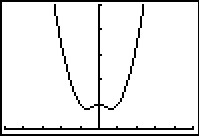
\includegraphics[width=2in]{./RationalsGraphics/Rationals09.jpg}

\end{tabular}

\end{ex}

\vspace{-.35in} \qed

\medskip

As usual, the authors offer no apologies for what may be construed as `pedantry' in this section.  We feel that the detail presented in this section is necessary to obtain a firm grasp of the concepts presented here and it also serves as an introduction to the methods employed in Calculus.  As we have said many times in the past, your instructor will decide how much, if any, of the kinds of details presented here are `mission critical' to your understanding of Precalculus. Without further delay, we present you with this section's Exercises.

\newpage

\subsection{Exercises}

In Exercises \ref{sixstepfirst} - \ref{sixsteplast}, use the six-step procedure to graph the rational function.  Be sure to draw any asymptotes as dashed lines.

\begin{multicols}{2}
\begin{enumerate}

\item $f(x) = \dfrac{4}{x + 2}$ \label{sixstepfirst}
\item $f(x) = \dfrac{5x}{6 - 2x}$

\setcounter{HW}{\value{enumi}}
\end{enumerate}
\end{multicols}

\begin{multicols}{2}
\begin{enumerate}
\setcounter{enumi}{\value{HW}}

\item $f(x) = \dfrac{1}{x^{2}}$
\item $f(x) = \dfrac{1}{x^{2} + x - 12}$

\setcounter{HW}{\value{enumi}}
\end{enumerate}
\end{multicols}

\begin{multicols}{2}
\begin{enumerate}
\setcounter{enumi}{\value{HW}}

\item $f(x) = \dfrac{2x - 1}{-2x^{2} - 5x + 3}$
\item $f(x) = \dfrac{x}{x^{2} + x - 12}$ \vphantom{$\dfrac{2x}{2x}$}

\setcounter{HW}{\value{enumi}}
\end{enumerate}
\end{multicols}

\begin{multicols}{2}
\begin{enumerate}
\setcounter{enumi}{\value{HW}}

\item $f(x) = \dfrac{4x}{x^2+4}$
\item $f(x) = \dfrac{4x}{x^2-4}$

\setcounter{HW}{\value{enumi}}
\end{enumerate}
\end{multicols}

\begin{multicols}{2}
\begin{enumerate}
\setcounter{enumi}{\value{HW}}

\item $f(x) = \dfrac{x^2-x-12}{x^2+x-6}$
\item $f(x) = \dfrac{3x^2-5x-2}{x^2-9}$

\setcounter{HW}{\value{enumi}}
\end{enumerate}
\end{multicols}

\begin{multicols}{2}
\begin{enumerate}
\setcounter{enumi}{\value{HW}}

\item $f(x) = \dfrac{x^2-x-6}{x+1}$

\item $f(x) = \dfrac{x^2-x}{3-x}$

\setcounter{HW}{\value{enumi}}
\end{enumerate}
\end{multicols}

\begin{multicols}{2}
\begin{enumerate}
\setcounter{enumi}{\value{HW}}

\item $f(x) = \dfrac{x^3+2x^2+x}{x^2-x-2}$

\item $f(x) = \dfrac{-x^{3} + 4x}{x^{2} - 9}$

\setcounter{HW}{\value{enumi}}
\end{enumerate}
\end{multicols}

\begin{multicols}{2}
\begin{enumerate}
\setcounter{enumi}{\value{HW}}

\item  $f(x) = \dfrac{x^3-2x^2+3x}{2x^2+2}$

\item \hspace{-0.1in}\footnote{Once you've done the six-step procedure, use your calculator to graph this function on the viewing window $[0, 12] \times [0, 0.25]$.  What do you see?} $f(x) = \dfrac{x^{2} - 2x + 1}{x^{3} + x^{2} - 2x}$ \label{sixsteplast}

\setcounter{HW}{\value{enumi}}
\end{enumerate}
\end{multicols}

In Exercises \ref{usetransratfirst} - \ref{usetransratlast}, graph the rational function by applying transformations to the graph of $y = \dfrac{1}{x}$.

\begin{multicols}{2}
\begin{enumerate}
\setcounter{enumi}{\value{HW}}

\item $f(x) = \dfrac{1}{x - 2}$ \label{usetransratfirst}
\item $g(x) = 1 - \dfrac{3}{x}$

\setcounter{HW}{\value{enumi}}
\end{enumerate}
\end{multicols}

\begin{multicols}{2}
\begin{enumerate}
\setcounter{enumi}{\value{HW}}


\item $h(x) = \dfrac{-2x + 1}{x}$ (Hint: Divide)
\item $j(x) = \dfrac{3x - 7}{x - 2}$ (Hint: Divide) \label{usetransratlast}


\setcounter{HW}{\value{enumi}}
\end{enumerate}
\end{multicols}


\begin{enumerate}
\setcounter{enumi}{\value{HW}}

\item Discuss with your classmates how you would graph $f(x) = \dfrac{ax + b}{cx + d}$.  What restrictions must be placed on $a, b, c$ and $d$ so that the graph is indeed a transformation of $y = \dfrac{1}{x}$?

\item In Example \ref{intropolyexample} in Section \ref{GraphsofPolynomials} we showed that $p(x) = \frac{4x+x^3}{x}$ is not a polynomial even though its formula reduced to $4 + x^{2}$ for $x \neq 0$.  However, it is a rational function similar to those studied in the section.  With the help of your classmates, graph $p(x)$.

\item Let $g(x) = \displaystyle \frac{x^{4} - 8x^{3} + 24x^{2} - 72x + 135}{x^{3} - 9x^{2} + 15x - 7}.\;$  With the help of your classmates, find the $x$- and $y$- intercepts of the graph of $g$.  Find the intervals on which the function is increasing, the intervals on which it is decreasing and the local extrema. Find all of the asymptotes of the graph of $g$ and any holes in the graph, if they exist.  Be sure to show all of your work including any polynomial or synthetic division.  Sketch the graph of $g$, using more than one picture if necessary to show all of the important features of the graph.

\setcounter{HW}{\value{enumi}}
\end{enumerate}

Example \ref{calcisneededhere} showed us that the six-step procedure cannot tell us everything of importance about the graph of a rational function.  Without Calculus, we need to use our graphing calculators to reveal the hidden mysteries of rational function behavior.  Working with your classmates, use a graphing calculator to examine the graphs of the rational functions given in Exercises \ref{rationalneedcalcfirst} - \ref{rationalneedcalclast}.  Compare and contrast their features.  Which features can the six-step process reveal and which features cannot be detected by it?

\begin{multicols}{4}
\begin{enumerate}
\setcounter{enumi}{\value{HW}}

\item $f(x) = \dfrac{1}{x^{2} + 1}$ \vphantom{$\dfrac{2x^{3}}{2x^{2}}$}  \label{rationalneedcalcfirst}
\item $f(x) = \dfrac{x}{x^{2} + 1}$ \vphantom{$\dfrac{2x^{3}}{2x^{2}}$}
\item $f(x) = \dfrac{x^{2}}{x^{2} + 1}$ \vphantom{$\dfrac{2x^{3}}{2x^{2}}$}
\item $f(x) = \dfrac{x^{3}}{x^{2} + 1}$ \vphantom{$\dfrac{2x^{3}}{2x^{2}}$} \label{rationalneedcalclast}

\setcounter{HW}{\value{enumi}}
\end{enumerate}
\end{multicols}

\newpage

\subsection{Answers}

\begin{enumerate}

\item \begin{multicols}{2} \raggedcolumns
$f(x) = \dfrac{4}{x + 2}$\\
Domain: $(-\infty, -2) \cup (-2, \infty)$\\
No $x$-intercepts\\
$y$-intercept: $(0, 2)$\\
Vertical asymptote: $x = -2$\\
As $x \rightarrow -2^{-}, \; f(x) \rightarrow -\infty$\\
As $x \rightarrow -2^{+}, \; f(x) \rightarrow \infty$\\
Horizontal asymptote: $y = 0$\\
As $x \rightarrow -\infty, \; f(x) \rightarrow 0^{-}$\\
As $x \rightarrow \infty, \; f(x) \rightarrow 0^{+}$\\

\begin{mfpic}[10]{-8}{6}{-6}{6}
\arrow \reverse \arrow \function{-8,-2.7,0.1}{4/(x+2)}
\arrow \reverse \arrow  \function{-1.3,6,0.1}{4/(x+2)}
\point[3pt]{(0,2)}
\dashed \polyline{(-2,-6), (-2,6)}
\tlabel[cc](6,-0.5){\scriptsize $x$}
\tlabel[cc](0.5,6){\scriptsize $y$}
\axes
\xmarks{-7 step 1 until 5}
\ymarks{-5 step 1 until 5}
\tiny
\tlpointsep{4pt}
\axislabels {x}{{$-7 \hspace{7pt}$} -7, {$-6 \hspace{7pt}$} -6, {$-5 \hspace{7pt}$} -5, {$-4 \hspace{7pt}$} -4, {$-3\hspace{7pt}$} -3, {$-2\hspace{7pt}$} -2, {$-1\hspace{7pt}$} -1,  {$1$} 1, {$2$} 2, {$3$} 3, {$4$} 4, {$5$} 5}
\axislabels {y}{{$-5$} -5, {$-4$} -4, {$-3$} -3, {$-2$} -2, {$-1$} -1, {$1$} 1, {$2$} 2, {$3$} 3, {$4$} 4, {$5$} 5}
\normalsize
\end{mfpic}

\end{multicols}

\item \begin{multicols}{2} \raggedcolumns 
$f(x) = \dfrac{5x}{6 - 2x}$\\
Domain: $(-\infty, 3) \cup (3, \infty)$\\
$x$-intercept: $(0, 0)$\\
$y$-intercept: $(0, 0)$\\
Vertical asymptote: $x = 3$\\
As $x \rightarrow 3^{-}, \; f(x) \rightarrow \infty$\\
As $x \rightarrow 3^{+}, \; f(x) \rightarrow -\infty$\\
Horizontal asymptote: $y = -\frac{5}{2}$\\
As $x \rightarrow -\infty, \; f(x) \rightarrow -\frac{5}{2}^{+}$\\
As $x \rightarrow \infty, \; f(x) \rightarrow -\frac{5}{2}^{-}$\\

\begin{mfpic}[10]{-4}{10}{-8}{4}
\arrow \reverse \arrow \function{-4,1.8,0.1}{(5*x)/(6 - (2*x))}
\arrow \reverse \arrow  \function{4.4,10,0.1}{(5*x)/(6 - (2*x))}
\point[3pt]{(0,0)}
\dashed \polyline{(3,-8), (3,4)}
\dashed \polyline{(-4,-2.5), (10,-2.5)}
\tlabel[cc](10,-0.5){\scriptsize $x$}
\tlabel[cc](0.5,4){\scriptsize $y$}
\axes
\xmarks{-3 step 1 until 9}
\ymarks{-7 step 1 until 3}
\tiny
\tlpointsep{4pt}
\axislabels {x}{{$-3\hspace{7pt}$} -3, {$-2\hspace{7pt}$} -2, {$-1\hspace{7pt}$} -1,  {$1$} 1, {$2$} 2, {$3$} 3, {$4$} 4, {$5$} 5, {$6$} 6, {$7$} 7, {$8$} 8, {$9$} 9}
\axislabels {y}{{$-7$} -7, {$-6$} -6, {$-5$} -5, {$-4$} -4, {$-3$} -3, {$-2$} -2, {$-1$} -1, {$1$} 1, {$2$} 2, {$3$} 3}
\normalsize
\end{mfpic}

\end{multicols}

\item \begin{multicols}{2} \raggedcolumns 
$f(x) = \dfrac{1}{x^{2}}$\\
Domain: $(-\infty, 0) \cup (0, \infty)$\\
No $x$-intercepts\\
No $y$-intercepts\\
Vertical asymptote: $x = 0$\\
As $x \rightarrow 0^{-}, \; f(x) \rightarrow \infty$\\
As $x \rightarrow 0^{+}, \; f(x) \rightarrow \infty$\\
Horizontal asymptote: $y = 0$\\
As $x \rightarrow -\infty, \; f(x) \rightarrow 0^{+}$\\
As $x \rightarrow \infty, \; f(x) \rightarrow 0^{+}$\\

\begin{mfpic}[15][20]{-5}{5}{-1}{6}
\arrow \reverse \arrow \function{-5,-0.42,0.1}{1/(x**2)}
\arrow \reverse \arrow  \function{0.42,5,0.1}{1/(x**2)}
\tlabel[cc](5,-0.5){\scriptsize $x$}
\tlabel[cc](0.5,6){\scriptsize $y$}
\axes
\xmarks{-4 step 1 until 4}
\ymarks{1 step 1 until 5}
\tiny
\tlpointsep{4pt}
\axislabels {x}{{$-4 \hspace{7pt}$} -4, {$-3\hspace{7pt}$} -3, {$-2\hspace{7pt}$} -2, {$-1\hspace{7pt}$} -1,  {$1$} 1, {$2$} 2, {$3$} 3, {$4$} 4}
\axislabels {y}{{$1$} 1, {$2$} 2, {$3$} 3, {$4$} 4, {$5$} 5}
\normalsize
\end{mfpic}

\end{multicols}

\pagebreak

\item \begin{multicols}{2} \raggedcolumns 
$f(x) = \dfrac{1}{x^{2} + x - 12} = \dfrac{1}{(x - 3)(x + 4)}$\\
Domain: $(-\infty, -4) \cup (-4, 3) \cup (3, \infty)$\\
No $x$-intercepts\\
$y$-intercept: $(0, -\frac{1}{12})$\\
Vertical asymptotes: $x = -4$ and $x = 3$\\
As $x \rightarrow -4^{-}, \; f(x) \rightarrow \infty$\\
As $x \rightarrow -4^{+}, \; f(x) \rightarrow -\infty$\\
As $x \rightarrow 3^{-}, \; f(x) \rightarrow -\infty$\\
As $x \rightarrow 3^{+}, \; f(x) \rightarrow \infty$\\
Horizontal asymptote: $y = 0$\\
As $x \rightarrow -\infty, \; f(x) \rightarrow 0^{+}$\\
As $x \rightarrow \infty, \; f(x) \rightarrow 0^{+}$\\

\begin{mfpic}[13][50]{-7}{5}{-1.5}{1.5}
\arrow \reverse \arrow \function{-6.5,-4.15,0.1}{1/((x**2) + x - 12)}
\arrow \reverse \arrow  \function{-3.85, 2.85,0.1}{1/((x**2) + x - 12)}
\arrow \reverse \arrow  \function{3.15,4.5,0.1}{1/((x**2) + x - 12)}
\point[3pt]{(0,-0.08333)}
\dashed \polyline{(3,-1.5), (3,1.5)}
\dashed \polyline{(-4,-1.5), (-4,1.5)}
\tlabel[cc](5,-0.1){\scriptsize $x$}
\tlabel[cc](0.5,1.5){\scriptsize $y$}
\axes
\xmarks{-6 step 1 until 4}
\ymarks{-1 step 1 until 1}
\tiny
\tlpointsep{4pt}
\axislabels {x}{{$-6 \hspace{7pt}$} -6, {$-5 \hspace{7pt}$} -5, {$-4 \hspace{7pt}$} -4, {$-3\hspace{7pt}$} -3, {$-2\hspace{7pt}$} -2, {$-1\hspace{7pt}$} -1,  {$1$} 1, {$2$} 2, {$3$} 3, {$4$} 4}
\axislabels {y}{{$-1$} -1, {$1$} 1}
\normalsize
\end{mfpic}

\end{multicols}

\item \begin{multicols}{2} \raggedcolumns 
$f(x) = \dfrac{2x - 1}{-2x^{2} - 5x + 3} = -\dfrac{2x - 1}{(2x - 1)(x + 3)}$\\
Domain: $(-\infty, -3) \cup (-3, \frac{1}{2}) \cup (\frac{1}{2}, \infty)$\\
No $x$-intercepts\\
$y$-intercept: $(0, -\frac{1}{3})$\\
$f(x) = \dfrac{-1}{x + 3}, \; x \neq \frac{1}{2}$\\
Hole in the graph at $(\frac{1}{2}, -\frac{2}{7})$\\
Vertical asymptote: $x = -3$\\
As $x \rightarrow -3^{-}, \; f(x) \rightarrow \infty$\\
As $x \rightarrow -3^{+}, \; f(x) \rightarrow -\infty$\\
Horizontal asymptote: $y = 0$\\
As $x \rightarrow -\infty, \; f(x) \rightarrow 0^{+}$\\
As $x \rightarrow \infty, \; f(x) \rightarrow 0^{-}$\\

\begin{mfpic}[15][45]{-8}{3}{-2}{2}
\arrow \reverse \arrow \function{-8,-3.5,0.1}{-1/(x+3)}
\arrow \reverse \arrow  \function{-2.5,3,0.1}{-1/(x+3)}
\dashed \polyline{(-3,-2), (-3,2)}
\gclear \ellipse{(0.5,-0.2857),0.1,0.033}
\ellipse{(0.5,-0.2857),0.1,0.033}
\point[3pt]{(0,-0.333)}
\tlabel[cc](3,0.1){\scriptsize $x$}
\tlabel[cc](0.5,2){\scriptsize $y$}
\axes
\xmarks{-7 step 1 until 2}
\ymarks{-1,1}
\tiny
\tlpointsep{4pt}
\axislabels {x}{{$-7 \hspace{7pt}$} -7, {$-6 \hspace{7pt}$} -6, {$-5 \hspace{7pt}$} -5, {$-4 \hspace{7pt}$} -4, {$-3\hspace{7pt}$} -3, {$-2\hspace{7pt}$} -2, {$-1\hspace{7pt}$} -1,  {$1$} 1, {$2$} 2}
\axislabels {y}{{$-1$} -1, {$1$} 1}
\normalsize
\end{mfpic}

\end{multicols}

\item \begin{multicols}{2} \raggedcolumns 
$f(x) = \dfrac{x}{x^{2} + x - 12} = \dfrac{x}{(x - 3)(x + 4)}$\\
Domain: $(-\infty, -4) \cup (-4, 3) \cup (3, \infty)$\\
$x$-intercept: $(0, 0)$\\
$y$-intercept: $(0, 0)$\\
Vertical asymptotes: $x = -4$ and $x = 3$\\
As $x \rightarrow -4^{-}, \; f(x) \rightarrow -\infty$\\
As $x \rightarrow -4^{+}, \; f(x) \rightarrow \infty$\\
As $x \rightarrow 3^{-}, \; f(x) \rightarrow -\infty$\\
As $x \rightarrow 3^{+}, \; f(x) \rightarrow \infty$\\
Horizontal asymptote: $y = 0$\\
As $x \rightarrow -\infty, \; f(x) \rightarrow 0^{-}$\\
As $x \rightarrow \infty, \; f(x) \rightarrow 0^{+}$\\

\begin{mfpic}[13][50]{-7}{6}{-1.5}{1.5}
\arrow \reverse \arrow \function{-6.5,-4.4,0.1}{x/((x**2) + x - 12)}
\arrow \reverse \arrow  \function{-3.6, 2.72,0.1}{x/((x**2) + x - 12)}
\arrow \reverse \arrow  \function{3.35,5.5,0.1}{x/((x**2) + x - 12)}
\point[3pt]{(0,0)}
\dashed \polyline{(3,-1.5), (3,1.5)}
\dashed \polyline{(-4,-1.5), (-4,1.5)}
\tlabel[cc](6,-0.1){\scriptsize $x$}
\tlabel[cc](0.5,1.5){\scriptsize $y$}
\axes
\xmarks{-6 step 1 until 5}
\ymarks{-1 step 1 until 1}
\tiny
\tlpointsep{4pt}
\axislabels {x}{{$-6 \hspace{7pt}$} -6, {$-5 \hspace{7pt}$} -5, {$-4 \hspace{7pt}$} -4, {$-3\hspace{7pt}$} -3, {$-2\hspace{7pt}$} -2, {$-1\hspace{7pt}$} -1,  {$1$} 1, {$2$} 2, {$3$} 3, {$4$} 4, {$5$} 5}
\axislabels {y}{{$-1$} -1, {$1$} 1}
\normalsize
\end{mfpic}

\end{multicols}

\item \begin{multicols}{2} \raggedcolumns
$f(x) = \dfrac{4x}{x^{2} + 4}$\\
Domain: $(-\infty,  \infty)$\\
$x$-intercept:  $(0,0)$\\
$y$-intercept:  $(0,0)$\\
No vertical asymptotes \\
No holes in the graph\\
Horizontal asymptote: $y = 0$ \\
As $x \rightarrow -\infty, f(x) \rightarrow 0^{-}$\\
As $x \rightarrow \infty, f(x) \rightarrow 0^{+}$\\

\begin{mfpic}[10][25]{-8}{8}{-2}{2}
\arrow \reverse \arrow \function{-8,8,0.1}{(4*x)/((x**2)+4)}
\point[3pt]{(0,0)}
\tlabel[cc](8,-0.5){\scriptsize $x$}
\tlabel[cc](0.5,2){\scriptsize $y$}
\axes
\xmarks{-7 step 1 until 7}
\ymarks{-1 step 1 until 1}
\tiny
\tlpointsep{4pt}
\axislabels {x}{{$-7 \hspace{7pt}$} -7,{$-6 \hspace{7pt}$} -6,{$-5 \hspace{7pt}$} -5, {$-4 \hspace{7pt}$} -4, {$-3\hspace{7pt}$} -3, {$-2\hspace{7pt}$} -2, {$-1\hspace{7pt}$} -1,  {$1$} 1, {$2$} 2, {$3$} 3, {$4$} 4, {$5$} 5, {$6$} 6, {$7$} 7}
\axislabels {y}{{$-1$} -1, {$1$} 1}
\normalsize
\end{mfpic}


\end{multicols}

\item \begin{multicols}{2} \raggedcolumns
$f(x) = \dfrac{4x}{x^{2} -4} = \dfrac{4x}{(x + 2)(x - 2)}$\\
Domain: $(-\infty, -2) \cup (-2, 2) \cup (2, \infty)$\\
$x$-intercept:  $(0,0)$\\
$y$-intercept:  $(0,0)$\\
Vertical asymptotes: $x = -2, x = 2$\\
As $x \rightarrow -2^{-}, f(x) \rightarrow -\infty$\\
As $x \rightarrow -2^{+}, f(x) \rightarrow \infty$\\
As $x \rightarrow 2^{-}, f(x) \rightarrow -\infty$\\
As $x \rightarrow 2^{+}, f(x) \rightarrow \infty$\\
No holes in the graph\\
Horizontal asymptote: $y = 0$ \\
As $x \rightarrow -\infty, f(x) \rightarrow 0^{-}$\\
As $x \rightarrow \infty, f(x) \rightarrow 0^{+}$\\

\begin{mfpic}[15]{-6}{6}{-6}{6}
\arrow \reverse \arrow \function{-6,-2.4,0.1}{(4*x)/((x**2)-4)}
\arrow \reverse \arrow \function{-1.64,1.64,0.1}{(4*x)/((x**2)-4)}
\arrow \reverse \arrow \function{-6,-2.4,0.1}{(4*x)/((x**2)-4)}
\arrow \reverse \arrow \function{2.4,6,0.1}{(4*x)/((x**2)-4)}
\point[3pt]{(0,0)}
\dashed \polyline{(-2,-6), (-2,6)}
\dashed \polyline{(2,-6), (2,6)}
\tlabel[cc](6,-0.5){\scriptsize $x$}
\tlabel[cc](0.5,6){\scriptsize $y$}
\axes
\xmarks{-5 step 1 until 5}
\ymarks{-5 step 1 until 5}
\tiny
\tlpointsep{4pt}
\axislabels {x}{{$-5 \hspace{7pt}$} -5, {$-4 \hspace{7pt}$} -4, {$-3\hspace{7pt}$} -3, {$-2\hspace{7pt}$} -2, {$-1\hspace{7pt}$} -1,  {$1$} 1, {$2$} 2, {$3$} 3, {$4$} 4, {$5$} 5}
\axislabels {y}{{$-5$} -5, {$-4$} -4, {$-3$} -3, {$-2$} -2, {$-1$} -1, {$1$} 1, {$2$} 2, {$3$} 3, {$4$} 4, {$5$} 5}
\normalsize
\end{mfpic}
\end{multicols}

\item \begin{multicols}{2} \raggedcolumns

$f(x) = \dfrac{x^2-x-12}{x^{2} +x - 6} = \dfrac{x-4}{x - 2} \, x \neq -3$\\
Domain: $(-\infty, -3) \cup (-3, 2) \cup (2, \infty)$\\
$x$-intercept:  $(4,0)$\\
$y$-intercept:  $(0,2)$\\
Vertical asymptote: $x = 2$\\
As $x \rightarrow 2^{-}, f(x) \rightarrow \infty$\\
As $x \rightarrow 2^{+}, f(x) \rightarrow -\infty$\\
Hole at $\left(-3, \frac{7}{5} \right)$ \\
Horizontal asymptote: $y = 1$ \\
As $x \rightarrow -\infty, f(x) \rightarrow 1^{+}$\\
As $x \rightarrow \infty, f(x) \rightarrow 1^{-}$\\


\begin{mfpic}[15]{-6}{6}{-6}{6}
\arrow \reverse \arrow \function{-6,1.5,0.1}{(x-4)/(x-2)}
\arrow \reverse \arrow \function{2.333,6,0.1}{(x-4)/(x-2)}
\point[3pt]{(4,0), (0,2)}
\gclear \circle{(-3,1.4),0.1}
\circle{(-3,1.4),0.1}
\dashed \polyline{(2,-6), (2,6)}
\dashed \polyline{(-6,1), (6,1)}
\tlabel[cc](6,-0.5){\scriptsize $x$}
\tlabel[cc](0.5,6){\scriptsize $y$}
\axes
\xmarks{-5 step 1 until 5}
\ymarks{-5 step 1 until 5}
\tiny
\tlpointsep{4pt}
\axislabels {x}{{$-5 \hspace{7pt}$} -5, {$-4 \hspace{7pt}$} -4, {$-3\hspace{7pt}$} -3, {$-2\hspace{7pt}$} -2, {$-1\hspace{7pt}$} -1,  {$1$} 1, {$2$} 2, {$3$} 3, {$4$} 4, {$5$} 5}
\axislabels {y}{{$-5$} -5, {$-4$} -4, {$-3$} -3, {$-2$} -2, {$-1$} -1, {$1$} 1, {$2$} 2, {$3$} 3, {$4$} 4, {$5$} 5}
\normalsize
\end{mfpic}

\end{multicols}

\pagebreak

\item \begin{multicols}{2} \raggedcolumns
$f(x) = \dfrac{3x^2-5x-2}{x^{2} -9} = \dfrac{(3x+1)(x-2)}{(x + 3)(x - 3)}$\\
Domain: $(-\infty, -3) \cup (-3, 3) \cup (3, \infty)$\\
$x$-intercepts: $\left(-\frac{1}{3}, 0 \right)$, $(2,0)$\\
$y$-intercept:  $\left(0, \frac{2}{9} \right)$\\
Vertical asymptotes: $x = -3, x = 3$\\
As $x \rightarrow -3^{-}, f(x) \rightarrow \infty$\\
As $x \rightarrow -3^{+}, f(x) \rightarrow -\infty$\\
As $x \rightarrow 3^{-}, f(x) \rightarrow -\infty$\\
As $x \rightarrow 3^{+}, f(x) \rightarrow \infty$\\
No holes in the graph\\
Horizontal asymptote: $y = 3$ \\
As $x \rightarrow -\infty, f(x) \rightarrow 3^{+}$\\
As $x \rightarrow \infty, f(x) \rightarrow 3^{-}$\\


\begin{mfpic}[9]{-10}{10}{-10}{10}
\arrow \reverse \arrow \function{-10,-3.9,0.1}{(3*(x**2)-5*x-2)/((x**2)-9)}
\arrow \reverse \arrow \function{-2.4,2.8,0.1}{(3*(x**2)-5*x-2)/((x**2)-9)}
\arrow \reverse \arrow \function{3.2,10,0.1}{(3*(x**2)-5*x-2)/((x**2)-9)}
\point[3pt]{(-0.3333,0), (2,0), (0,0.2222)}
\dashed \polyline{(3,-10), (3,10)}
\dashed \polyline{(-3,-10), (-3,10)}
\dashed \polyline{(-10,3), (10,3)}
\tlabel[cc](10,-0.5){\scriptsize $x$}
\tlabel[cc](0.5,10){\scriptsize $y$}
\axes
\xmarks{-9 step 1 until 9}
\ymarks{-9 step 1 until 9}
\tiny
\tlpointsep{4pt}
\axislabels {x}{{$-9 \hspace{7pt}$} -9,{$-8 \hspace{7pt}$} -8,{$-7 \hspace{7pt}$} -7,{$-7 \hspace{7pt}$} -7,{$-6 \hspace{7pt}$} -6,{$-5 \hspace{7pt}$} -5, {$-4 \hspace{7pt}$} -4, {$-3\hspace{7pt}$} -3, {$-2\hspace{7pt}$} -2, {$-1\hspace{7pt}$} -1,  {$1$} 1, {$2$} 2, {$3$} 3, {$4$} 4, {$5$} 5, {$6$} 6, {$7$} 7, {$8$} 8, {$9$} 9}
\axislabels {y}{{$-9$} -9,{$-8$} -8,{$-7$} -7,{$-6$} -6,{$-5$} -5, {$-4$} -4, {$-3$} -3, {$-2$} -2, {$-1$} -1, {$1$} 1, {$2$} 2, {$3$} 3, {$4$} 4, {$5$} 5, {$6$} 6, {$7$} 7, {$8$} 8, {$9$} 9}
\normalsize
\end{mfpic}

\end{multicols}

\item \begin{multicols}{2} \raggedcolumns 
$f(x) = \dfrac{x^2-x-6}{x+1} = \dfrac{(x-3)(x+2)}{x+1}$\\
Domain: $(-\infty, -1) \cup (-1, \infty)$\\
$x$-intercepts:  $(-2,0)$, $(3,0)$\\
$y$-intercept:  $(0,-6)$\\
Vertical asymptote: $x = -1$\\
As $x \rightarrow -1^{-}, f(x) \rightarrow \infty$\\
As $x \rightarrow -1^{+}, f(x) \rightarrow -\infty$\\
Slant asymptote: $y = x-2$ \\
As $x \rightarrow -\infty$, the graph is above $y=x-2$\\
As $x \rightarrow \infty$, the graph is below $y=x-2$\\

\begin{mfpic}[10][8]{-5}{5}{-10}{10}
\arrow \reverse \arrow \function{-5,-1.3,0.1}{((x-3)*(x+2))/(x+1)}
\arrow \reverse \arrow \function{-0.45,5,0.1}{((x-3)*(x+2))/(x+1)}
\dashed \function{-5,5,0.1}{x-2}
\point[3pt]{(0,-6), (3,0), (-2,0)}
\dashed \polyline{(-1,-10), (-1,10)}
\tlabel[cc](5,-0.5){\scriptsize $x$}
\tlabel[cc](0.5,10){\scriptsize $y$}
\axes
\xmarks{-4 step 1 until 4}
\ymarks{-9 step 1 until 9}
\tiny
\tlpointsep{4pt}
\axislabels {x}{{$-4 \hspace{7pt}$} -4, {$-3 \hspace{7pt}$} -3, {$-2 \hspace{7pt}$} -2,   {$-1 \hspace{7pt}$} -1,{$1$} 1, {$2$} 2, {$3$} 3, {$4$} 4}
\axislabels {y}{{$-6$} -6, {$-4$} -4, {$-2$} -2, {$2$} 2, {$4$} 4, {$6$} 6, {$8$} 8, {$9$} 9, {$1$} 1, {$3$} 3, {$5$} 5, {$7$} 7}
\normalsize
\end{mfpic}

\end{multicols}

\item \begin{multicols}{2} \raggedcolumns 
$f(x) = \dfrac{x^2-x}{3-x} = \dfrac{x(x-1)}{3-x}$\\
Domain: $(-\infty, 3) \cup (3, \infty)$\\
$x$-intercepts:  $(0,0)$, $(1,0)$\\
$y$-intercept:  $(0,0)$\\
Vertical asymptote: $x = 3$\\
As $x \rightarrow 3^{-}, f(x) \rightarrow \infty$\\
As $x \rightarrow 3^{+}, f(x) \rightarrow -\infty$\\
Slant asymptote: $y = -x-2$ \\
As $x \rightarrow -\infty$, the graph is above $y=-x-2$\\
As $x \rightarrow \infty$, the graph is below $y=-x-2$\\

\begin{mfpic}[8][6]{-9}{11}{-20}{11}
\arrow \reverse \arrow \function{-9,2.6,0.1}{(x*(x-1))/(3-x)}
\arrow \reverse \arrow \function{3.4,11,0.1}{(x*(x-1))/(3-x)}
\dashed \function{-9,11,0.1}{-x-2}
\point[3pt]{(0,0),(1,0)}
\dashed \polyline{(3,-20), (3,11)}
\tlabel[cc](11,-0.5){\scriptsize $x$}
\tlabel[cc](0.5,11){\scriptsize $y$}
\axes
\xmarks{-8 step 1 until 9}
\ymarks{-19 step 1 until 10}
\tiny
\tlpointsep{4pt}
\axislabels {x}{{$-8 \hspace{7pt}$} -8,{$-7 \hspace{7pt}$} -7,{$-6 \hspace{7pt}$} -6,{$-5 \hspace{7pt}$} -5,{$-4 \hspace{7pt}$} -4, {$-3 \hspace{7pt}$} -3, {$-2 \hspace{7pt}$} -2,   {$-1 \hspace{7pt}$} -1,{$1$} 1, {$2$} 2, {$3$} 3, {$4$} 4, {$5$} 5, {$6$} 6, {$7$} 7, {$8$} 8, {$9$} 9, {$10$} 10}
\axislabels {y}{{$-12$} -12,{$-14$} -14,{$-16$} -16,{$-18$} -18,{$-10$} -10, {$-8$} -8, {$-6$} -6, {$-4$} -4, {$-2$} -2, {$2$} 2, {$4$} 4, {$6$} 6, {$8$} 8}
\normalsize
\end{mfpic}

\end{multicols}


\item \begin{multicols}{2} \raggedcolumns
$f(x) = \dfrac{x^3+2x^2+x}{x^{2} -x-2} = \dfrac{x(x+1)}{x - 2} \, x \neq -1$\\
Domain: $(-\infty, -1) \cup (-1, 2) \cup (2, \infty)$\\
$x$-intercept:  $(0,0)$\\
$y$-intercept:  $(0,0)$\\
Vertical asymptote: $x = 2$\\
As $x \rightarrow 2^{-}, f(x) \rightarrow -\infty$\\
As $x \rightarrow 2^{+}, f(x) \rightarrow \infty$\\
Hole at $(-1,0)$ \\
Slant asymptote: $y = x+3$ \\
As $x \rightarrow -\infty$, the graph is below $y=x+3$ \\
As $x \rightarrow \infty$, the graph is above $y=x+3$\\

\begin{mfpic}[8][6]{-10}{10}{-11}{20}
\arrow \reverse \arrow \function{-10,1.6,0.1}{(x*(x+1))/(x-2)}
\arrow \reverse \arrow \function{2.4,10,0.1}{(x*(x+1))/(x-2)}
\dashed \function{-10,10,0.1}{x+3}
\point[3pt]{(0,0)}
\dashed \polyline{(2,-11), (2,20)}
\tlabel[cc](10,-0.5){\scriptsize $x$}
\tlabel[cc](0.5,20){\scriptsize $y$}
\axes
\xmarks{-9 step 1 until 9}
\gclear \ellipse{(-1,0),0.2,0.27}
\ellipse{(-1,0),0.2,0.27}
\ymarks{-11 step 1 until 19}
\tiny
\tlpointsep{4pt}
\axislabels {x}{{$-9 \hspace{7pt}$} -9,{$-8 \hspace{7pt}$} -8,{$-7 \hspace{7pt}$} -7,{$-6 \hspace{7pt}$} -6,{$-5 \hspace{7pt}$} -5,{$-4 \hspace{7pt}$} -4, {$-3 \hspace{7pt}$} -3, {$-2 \hspace{7pt}$} -2,   {$-1 \hspace{7pt}$} -1,{$1$} 1, {$2$} 2, {$3$} 3, {$4$} 4, {$5$} 5, {$6$} 6, {$7$} 7, {$8$} 8, {$9$} 9}
\axislabels {y}{{$-10$} -10, {$-8$} -8, {$-6$} -6, {$-4$} -4, {$-2$} -2, {$2$} 2, {$4$} 4, {$6$} 6, {$8$} 8, {$10$} 10, {$12$} 12, {$14$} 14, {$16$} 16, {$18$} 18}
\normalsize
\end{mfpic}

\end{multicols}


\item \begin{multicols}{2} \raggedcolumns 
$f(x) = \dfrac{-x^{3} + 4x}{x^{2} - 9}$\\
Domain: $(-\infty, -3) \cup (-3, 3) \cup (3, \infty)$\\
$x$-intercepts: $(-2, 0), (0, 0), (2, 0)$\\
$y$-intercept: $(0, 0)$\\
Vertical asymptotes: $x = -3, x = 3$\\
As $x \rightarrow -3^{-}, \; f(x) \rightarrow \infty$\\
As $x \rightarrow -3^{+}, \; f(x) \rightarrow -\infty$\\
As $x \rightarrow 3^{-}, \; f(x) \rightarrow \infty$\\
As $x \rightarrow 3^{+}, \; f(x) \rightarrow -\infty$\\
Slant asymptote: $y = -x$\\
As $x \rightarrow -\infty$, the graph is above $y=-x$\\
As $x \rightarrow \infty$, the graph is below $y=-x$\\

\begin{mfpic}[10]{-7}{7}{-8}{8}
\arrow \reverse \arrow \function{-7,-3.7,0.1}{((4*x) - (x**3))/((x**2) - 9)}
\arrow \reverse \arrow \function{-2.76,2.76,0.1}{((4*x) - (x**3))/((x**2) - 9)}
\arrow \reverse \arrow  \function{3.7,7,0.1}{((4*x) - (x**3))/((x**2) - 9)}
\point[3pt]{(-2,0), (0,0), (2, 0)}
\dashed \polyline{(-3,-8), (-3,8)}
\dashed \polyline{(3,-8), (3,8)}
\dashed \function{-7,7,0.1}{-x}
\tlabel[cc](7,-0.5){\scriptsize $x$}
\tlabel[cc](0.5,8){\scriptsize $y$}
\axes
\xmarks{-6 step 1 until 6}
\ymarks{-7 step 1 until 7}
\tiny
\tlpointsep{4pt}
\axislabels {x}{{$-6 \hspace{7pt}$} -6, {$-5 \hspace{7pt}$} -5, {$-4 \hspace{7pt}$} -4, {$-3\hspace{7pt}$} -3, {$-2\hspace{7pt}$} -2, {$-1\hspace{7pt}$} -1,  {$1$} 1, {$2$} 2, {$3$} 3, {$4$} 4, {$5$} 5, {$6$} 6}
\axislabels {y}{{$-7$} -7, {$-6$} -6, {$-5$} -5, {$-4$} -4, {$-3$} -3, {$-2$} -2, {$-1$} -1, {$1$} 1, {$2$} 2, {$3$} 3, {$4$} 4, {$5$} 5, {$6$} 6, {$7$} 7}
\normalsize
\end{mfpic}

\end{multicols}

\item \begin{multicols}{2} \raggedcolumns 
$f(x) = \dfrac{x^3-2x^2+3x}{2x^2+2}$\\
Domain: $(-\infty,\infty)$\\
$x$-intercept: $(0,0)$\\
$y$-intercept:  $(0,0)$\\
Slant asymptote: $y = \frac{1}{2}x-1$\\
As $x \rightarrow -\infty$, the graph is below $y = \frac{1}{2}x-1$\\
As $x \rightarrow \infty$, the graph is above $y = \frac{1}{2}x-1$\\

\begin{mfpic}[15]{-5}{5}{-3}{3}
\arrow \reverse \arrow \function{-5,5,0.1}{(x*((x**2)-2*x+3))/(2*(x**2)+2)}
\dashed \polyline{(-5,-3.5), (5,1.5)}
\tlabel[cc](5,-0.5){\scriptsize $x$}
\tlabel[cc](0.5,3){\scriptsize $y$}
\axes
\xmarks{-4,-3,-2,-1,2,3,4}
\ymarks{-2 step 1 until 2}
\tiny
\tlpointsep{4pt}
\axislabels {x}{{$-4 \hspace{7pt}$} -4, {$-3\hspace{7pt}$} -3, {$-2\hspace{7pt}$} -2, {$-1\hspace{7pt}$} -1, {$1$} 1, {$2$} 2, {$3$} 3, {$4$} 4}
\axislabels {y}{{$-2$} -2, {$-1$} -1, {$1$} 1, {$2$} 2}
\normalsize
\end{mfpic}

\end{multicols}

\pagebreak

\item \begin{multicols}{2} \raggedcolumns 
$f(x) = \dfrac{x^{2} - 2x + 1}{x^{3} + x^{2} - 2x}$\\
Domain: $(-\infty, -2) \cup (-2, 0) \cup (0, 1) \cup (1, \infty)$\\
$f(x) = \dfrac{x - 1}{x(x + 2)}, \; x \neq 1$\\
No $x$-intercepts\\
No $y$-intercepts\\
Vertical asymptotes: $x = -2$ and $x = 0$\\
As $x \rightarrow -2^{-}, \; f(x) \rightarrow -\infty$\\
As $x \rightarrow -2^{+}, \; f(x) \rightarrow \infty$\\
As $x \rightarrow 0^{-}, \; f(x) \rightarrow \infty$\\
As $x \rightarrow 0^{+}, \; f(x) \rightarrow -\infty$\\
Hole in the graph at $(1, 0)$\\
Horizontal asymptote: $y = 0$\\
As $x \rightarrow -\infty, \; f(x) \rightarrow 0^{-}$\\
As $x \rightarrow \infty, \; f(x) \rightarrow 0^{+}$\\

\begin{mfpic}[15]{-6}{6}{-6}{6}
\arrow \reverse \arrow \function{-6,-2.25,0.1}{(x-1)/((x**2) + (2*x))}
\arrow \reverse \arrow  \function{-1.73,-0.1,0.1}{(x-1)/((x**2) + (2*x))}
\arrow \reverse \arrow  \function{0.08,6,0.1}{(x-1)/((x**2) + (2*x))}
\dashed \polyline{(-2,-6), (-2,6)}
\tlabel[cc](6,-0.5){\scriptsize $x$}
\tlabel[cc](0.5,6){\scriptsize $y$}
\axes
\xmarks{-5,-4,-3,-2,-1,2,3,4,5}
\ymarks{-5 step 1 until 5}
\tiny
\tlpointsep{4pt}
\axislabels {x}{{$-5 \hspace{7pt}$} -5, {$-4 \hspace{7pt}$} -4, {$-3\hspace{7pt}$} -3, {$-2\hspace{7pt}$} -2, {$-1\hspace{7pt}$} -1, {$1$} 1, {$2$} 2, {$3$} 3, {$4$} 4, {$5$} 5}
\axislabels {y}{{$-5$} -5, {$-4$} -4, {$-3$} -3, {$-2$} -2, {$-1$} -1, {$1$} 1, {$2$} 2, {$3$} 3, {$4$} 4, {$5$} 5}
\normalsize
\gclear \circle{(1,0),0.1}
\circle{(1,0),0.1}
\end{mfpic}

\end{multicols}

\item \begin{multicols}{2} \raggedcolumns 
$f(x) = \dfrac{1}{x - 2}$\\
Shift the graph of $y = \dfrac{1}{x}$ \\
to the right 2 units.\\

\begin{mfpic}[18]{-2}{6}{-4}{4}
\arrow \reverse \arrow \function{-2,1.75,0.1}{1/(x-2)}
\arrow \reverse \arrow  \function{2.25,6,0.1}{1/(x-2)}
\point[3pt]{(1,-1), (3,1)}
\dashed \polyline{(2,-4), (2,4)}
\tlabel[cc](6,-0.5){\scriptsize $x$}
\tlabel[cc](0.5,4){\scriptsize $y$}
\axes
\xmarks{-1 step 1 until 5}
\ymarks{-3 step 1 until 3}
\tiny
\tlpointsep{4pt}
\axislabels {x}{{$-1\hspace{7pt}$} -1,  {$1$} 1, {$2$} 2, {$3$} 3, {$4$} 4, {$5$} 5}
\axislabels {y}{{$-3$} -3, {$-2$} -2, {$-1$} -1, {$1$} 1, {$2$} 2, {$3$} 3}
\normalsize
\end{mfpic}

\end{multicols}

\item \begin{multicols}{2} \raggedcolumns 
$g(x) = 1 - \dfrac{3}{x}$\\
Vertically stretch the graph of $y = \dfrac{1}{x}$\\
by a factor of 3.\\
Reflect the graph of $y = \dfrac{3}{x}$\\
about the $x$-axis.\\
Shift the graph of $y = -\dfrac{3}{x}$\\
up 1 unit.\\

\begin{mfpic}[10]{-7}{7}{-6}{8}
\arrow \reverse \arrow \function{-7,-0.45,0.1}{1 - (3/x)}
\arrow \reverse \arrow  \function{0.45,7,0.1}{1 - (3/x)}
\point[3pt]{(-3,2), (-1,4), (1,-2), (3,0)}
\dashed \polyline{(-7,1), (7,1)}
\tlabel[cc](7,-0.5){\scriptsize $x$}
\tlabel[cc](0.5,8){\scriptsize $y$}
\axes
\xmarks{-6 step 1 until 6}
\ymarks{-5 step 1 until 7}
\tiny
\tlpointsep{4pt}
\axislabels {x}{{$-6 \hspace{7pt}$} -6, {$-5 \hspace{7pt}$} -5, {$-4 \hspace{7pt}$} -4, {$-3\hspace{7pt}$} -3, {$-2\hspace{7pt}$} -2, {$-1\hspace{7pt}$} -1,  {$1$} 1, {$2$} 2, {$3$} 3, {$4$} 4, {$5$} 5, {$6$} 6}
\axislabels {y}{{$-5$} -5, {$-4$} -4, {$-3$} -3, {$-2$} -2, {$-1$} -1, {$1$} 1, {$2$} 2, {$3$} 3, {$4$} 4, {$5$} 5, {$6$} 6, {$7$} 7}
\normalsize
\end{mfpic}

\end{multicols}

\pagebreak

\item \begin{multicols}{2} \raggedcolumns 
$h(x) = \dfrac{-2x + 1}{x} = -2 + \dfrac{1}{x}$\\
Shift the graph of $y = \dfrac{1}{x}$\\
down 2 units.\\

\begin{mfpic}[18]{-4}{4}{-6}{2}
\arrow \reverse \arrow \function{-4,-0.25,0.1}{(1/x)-2}
\arrow \reverse \arrow  \function{0.25,4,0.1}{(1/x)-2}
\point[3pt]{(1,-1), (-1,-3)}
\dashed \polyline{(-4,-2), (4,-2)}
\tlabel[cc](4,-0.5){\scriptsize $x$}
\tlabel[cc](-0.5,2){\scriptsize $y$}
\axes
\xmarks{-3 step 1 until 3}
\ymarks{-5 step 1 until 1}
\tiny
\tlpointsep{4pt}
\axislabels {x}{{$-3\hspace{7pt}$} -3, {$-2\hspace{7pt}$} -2, {$-1\hspace{7pt}$} -1,  {$1$} 1, {$2$} 2, {$3$} 3}
\axislabels {y}{{$-5$} -5, {$-4$} -4, {$-3$} -3, {$-2$} -2, {$-1$} -1, {$1$} 1}
\normalsize
\end{mfpic}

\end{multicols}

\item \begin{multicols}{2} \raggedcolumns  
$j(x) = \dfrac{3x - 7}{x - 2} = 3 - \dfrac{1}{x - 2}$\\
Shift the graph of $y = \dfrac{1}{x}$\\
to the right 2 units.\\
Reflect the graph of $y = \dfrac{1}{x - 2}$\\
about the $x$-axis.\\
Shift the graph of $y = -\dfrac{1}{x - 2}$\\
up 3 units.\\

\begin{mfpic}[15]{-4}{6}{-2}{8}
\arrow \reverse \arrow \function{-4,1.8,0.1}{3 - (1/(x - 2))}
\arrow \reverse \arrow  \function{2.2,6,0.1}{3 - (1/(x - 2))}
\point[3pt]{(3,2), (1,4)}
\dashed \polyline{(-4,3), (6,3)}
\dashed \polyline{(2,-2), (2,8)}
\tlabel[cc](6,-0.5){\scriptsize $x$}
\tlabel[cc](0.5,8){\scriptsize $y$}
\axes
\xmarks{-3 step 1 until 5}
\ymarks{-1 step 1 until 7}
\tiny
\tlpointsep{4pt}
\axislabels {x}{{$-3\hspace{7pt}$} -3, {$-2\hspace{7pt}$} -2, {$-1\hspace{7pt}$} -1,  {$1$} 1, {$2$} 2, {$3$} 3, {$4$} 4, {$5$} 5}
\axislabels {y}{{$-1$} -1, {$1$} 1, {$2$} 2, {$3$} 3, {$4$} 4, {$5$} 5, {$6$} 6, {$7$} 7}
\normalsize
\end{mfpic}

\end{multicols}

\end{enumerate}

\closegraphsfile

\newpage

\section{Rational Inequalities and Applications}

\mfpicnumber{1}
\opengraphsfile{RationalIneq}

\setcounter{footnote}{0}

\label{RationalIneq}

In this section, we solve equations and inequalities involving rational functions and explore associated application problems. Our first example showcases the critical difference in procedure between solving a rational equation and a rational inequality.

\begin{ex}  $~$

\begin{multicols}{2}
\begin{enumerate}

\item  Solve $\dfrac{x^3-2x+1}{x-1} = \dfrac{1}{2}x-1$.

\item  Solve $\dfrac{x^3-2x+1}{x-1} \geq \dfrac{1}{2}x-1$.

\setcounter{HW}{\value{enumi}}
\end{enumerate}
\end{multicols}

\begin{enumerate}
\setcounter{enumi}{\value{HW}}

\item  Use your calculator to graphically check your answers to 1 and 2.

\end{enumerate}

{ \bf Solution.} 

\begin{enumerate}

\item  To solve the equation, we clear denominators

\[ \begin{array}{rclr}

\dfrac{x^3-2x+1}{x-1} & = & \dfrac{1}{2}x-1 & \\ [10pt]

\left(\dfrac{x^3-2x+1}{x-1}\right) \cdot 2(x-1) & = & \left( \dfrac{1}{2}x-1 \right) \cdot 2(x-1) & \\ [10pt]

2x^3 - 4x + 2 & = & x^2-3x+2 & \mbox{expand} \\

2x^3 -x^2 - x & = & 0 & \\

x(2x+1)(x-1) & = & 0 & \mbox{factor}\\

x & = & -\frac{1}{2}, \, 0, \, 1 & \\


\end{array}\]

Since we cleared denominators, we need to check for extraneous solutions.  Sure enough, we see that $x=1$ does not satisfy the original equation and must be discarded.  Our solutions are $x=-\frac{1}{2}$ and $x=0$.

\item  To solve the inequality, it may be tempting to begin as we did with the equation $-$ namely by multiplying both sides by the quantity $(x-1)$.  The problem is that, depending on $x$, $(x-1)$ may be positive (which doesn't affect the inequality) or $(x-1)$ could be negative (which would reverse the inequality).  Instead of working by cases, we collect all of the terms on one side of the inequality with $0$ on the other and make a sign diagram using the technique given on page \pageref{rationalsigndiagram} in Section \ref{RationalGraphs}.

\[ \begin{array}{rclr}

\dfrac{x^3-2x+1}{x-1} & \geq & \dfrac{1}{2}x-1 & \\ [10pt]

\dfrac{x^3-2x+1}{x-1}  - \dfrac{1}{2} x + 1& \geq & 0& \\ [10pt]

\dfrac{2\left(x^3-2x+1\right)-x(x-1)+1(2(x-1))}{2(x-1)} & \geq & 0 & \mbox{get a common denominator} \\ [10pt]

\dfrac{2x^3-x^2-x}{2x-2} & \geq & 0 & \mbox{expand} \\

\end{array} \]

Viewing the left hand side as a rational function $r(x)$ we make a sign diagram.  The only value excluded from the domain of $r$ is $x=1$ which is the solution to $2x-2=0$.  The zeros of $r$ are the solutions to $2x^3-x^2-x=0$, which we have already found to be $x=0$, $x=-\frac{1}{2}$ and $x=1$, the latter was discounted as a zero because it is not in the domain.  Choosing test values in each test interval, we construct the sign diagram below. 

\begin{center}

\begin{mfpic}[10]{-6}{6}{-2}{2}
\arrow \reverse \arrow \polyline{(-6,0),(6,0)}
\xmarks{-3,0,3}
\tlpointsep{6pt}
\axislabels {x}{{$-\frac{1}{2} \hspace{7pt}$ } -3, {$0$} 0, {$1$} 3 }
\tlabel[cc](-4.5,1){$(+)$}
\tlabel[cc](-3,1){$0$}
\tlabel[cc](-1.5,1){$(-)$}
\tlabel[cc](0,1){$0$}
\tlabel[cc](1.5,1){$(+)$}
\tlabel[cc](3,1){\textinterrobang}
\tlabel[cc](4.5,1){$(+)$}
\end{mfpic} 

\end{center}

We are interested in where $r(x) \geq 0$.  We find $r(x) > 0$, or $(+)$, on the intervals $\left(-\infty, -\frac{1}{2}\right)$, $(0,1)$ and $(1, \infty)$.  We add to these intervals the zeros of $r$, $-\frac{1}{2}$ and $0$, to get our final solution:  $\left( - \infty, -\frac{1}{2} \right] \cup [0,1) \cup (1, \infty)$.

\item  Geometrically, if we set $f(x) = \frac{x^3-2x+1}{x-1}$ and $g(x) = \frac{1}{2} x -1$, the solutions to $f(x)=g(x)$ are the $x$-coordinates of the points where the graphs of $y=f(x)$ and $y=g(x)$ intersect.  The solution to $f(x) \geq g(x)$ represents not only where the graphs meet, but the intervals over which the graph of $y=f(x)$ is above ($>$) the graph of $g(x)$. We obtain the graphs below.  

\begin{center}

\begin{tabular}{cc}

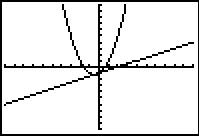
\includegraphics[width=2in]{./RationalsGraphics/Rationals10.jpg} \hspace{0.75in} & 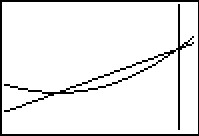
\includegraphics[width=2in]{./RationalsGraphics/Rationals11.jpg} \\


\end{tabular}
\end{center} 

The `Intersect' command confirms that the graphs cross when $x=-\frac{1}{2}$ and $x=0$.  It is clear from the calculator that the graph of $y=f(x)$ is above the graph of $y=g(x)$ on $\left(-\infty, -\frac{1}{2}\right)$ as well as on $(0,\infty)$.  According to the calculator, our solution is then $\left(-\infty, -\frac{1}{2}\right] \cup [0, \infty)$ which \textit{almost} matches the answer we found analytically.  We have to remember that $f$ is not defined at $x=1$, and, even though it isn't shown on the calculator, there is a hole\footnote{There is no asymptote at $x=1$ since the graph is well behaved near $x=1$.  According to Theorem \ref{vavshole}, there  must be a hole there.}  in the graph of $y=f(x)$ when $x=1$ which is why $x=1$ is not part of our final answer. \qed

\end{enumerate}
\end{ex}  

Next, we explore how rational equations can be used to solve some classic problems involving rates.

\begin{ex}  \label{upstreamdownstreamex}  Carl decides to explore the Meander River, the location of several recent Sasquatch sightings.  From camp, he canoes downstream five miles to check out a purported Sasquatch nest.  Finding nothing, he immediately turns around, retraces his route (this time traveling upstream), and returns to camp 3 hours after he left.  If Carl canoes at a rate  of 6 miles per hour in still water, how fast was the Meander River flowing on that day?

\smallskip

{\bf Solution.}  We are given information about distances, rates (speeds) and times.  The basic principle relating these quantities is: \[ \text{distance} = \text{rate} \cdot \text{time}\]  The first observation to make, however, is that the distance, rate and time given to us aren't `compatible':  the distance given is the distance for only \textit{part} of the trip,  the rate given is the speed Carl can canoe in still water, not in a flowing river, and  the time given is the duration of the \textit{entire} trip.  Ultimately, we are after the speed of the river, so let's call that $R$ measured in miles per hour to be consistent with the other rate given to us.  To get started, let's divide the trip into its two parts:  the initial trip downstream and the return trip upstream.  For the downstream trip, all we know is that the distance traveled is $5$ miles.

\[ \begin{array}{rcl}

\text{distance downstream} & = & \text{rate traveling downstream} \cdot \text{time traveling downstream} \\

5 \, \text{miles} & = & \text{rate traveling downstream} \cdot \text{time traveling downstream} \\ \end{array} \]

Since the return trip upstream followed the same route as the trip downstream, we know that the distance traveled upstream is also 5 miles.

\[ \begin{array}{rcl}

\text{distance upstream} & = & \text{rate traveling upstream} \cdot \text{time traveling upstream} \\

5 \, \text{miles} & = & \text{rate traveling upstream} \cdot \text{time traveling upstream} \\ \end{array} \]

We are told Carl can canoe at a  rate of $6$ miles per hour in still water.  How does this figure into the rates traveling upstream and downstream?  The speed the canoe travels in the river is a combination of the speed at which Carl can propel the canoe in still water, 6 miles per hour,  and the speed of the river, which we're calling $R$. When traveling downstream, the river is helping Carl along, so we \textit{add} these two speeds: 

\[ \begin{array}{rcl}

\text{rate traveling downstream} & = & \text{rate Carl propels the canoe} + \text{speed of the river} \\

 & = & 6 \frac{\text{miles}}{\text{hour}} + R \frac{\text{miles}}{\text{hour}} \\ \end{array} \]
 
 So our downstream speed is $(6+R) \frac{\text{miles}}{\text{hour}}$.  Substituting this into our `distance-rate-time' equation for the downstream part of the trip, we get:
 
 \[ \begin{array}{rcl}

5 \, \text{miles} & = & \text{rate traveling downstream} \cdot \text{time traveling downstream} \\ 

5 \, \text{miles} & = & (6+R) \frac{\text{miles}}{\text{hour}} \cdot \text{time traveling downstream} \\ 	\end{array} \]

 When traveling upstream, Carl works against the current.  Since the canoe manages to travel upstream,  the speed Carl can canoe in still water is greater than the river's speed, so we \textit{subtract} the river's speed \textit{from} Carl's canoing speed to get:
 
 \[ \begin{array}{rcl}

\text{rate traveling upstream} & = & \text{rate Carl propels the canoe} - \text{river speed} \\

 & = & 6 \frac{\text{miles}}{\text{hour}} - R \frac{\text{miles}}{\text{hour}} \\ \end{array} \]
 
Proceeding as before, we get
 
 \[ \begin{array}{rcl}

5 \, \text{miles} & = & \text{rate traveling upstream} \cdot \text{time traveling upstream} \\ 

5 \, \text{miles} & = & (6 - R) \frac{\text{miles}}{\text{hour}} \cdot \text{time traveling upstream} \\ 	\end{array} \]
 
The last piece of information given to us is that the total trip lasted $3$ hours.  If we let $t_{\text{down}}$ denote the time of the downstream trip and $t_{\text{up}}$ the time of the upstream trip, we have:    $t_{\text{down}} + t_{\text{up}} = 3 \, \text{hours}$.  Substituting $t_{\text{down}}$ and $t_{\text{up}}$ into the `distance-rate-time' equations, we get (suppressing the units) \textit{three} equations in \textit{three} unknowns:\footnote{This is called a \textit{system} of equations.  No doubt, you've had experience with these things before, and we will study systems in greater detail in Chapter \ref{Matrices}.} \[\left\{\begin{array}{lrcl}   E1 & (6+R) \, t_{\text{down}} & = & 5 \\ E2 & (6-R) \, t_{\text{up}} & = & 5 \\ E3 & t_{\text{down}} + t_{\text{up}} & = & 3 \end{array} \right.\]

Since we are ultimately after $R$, we need to use these three equations to get at least one equation involving only $R$.  To that end, we solve $E1$ for $t_{\text{down}}$ by dividing both sides\footnote{While we usually discourage dividing both sides of an equation by a variable expression, we know $(6+R) \neq 0$ since otherwise we couldn't possibly multiply it by $t_{\text{down}}$ and get $5$.} by the quantity $(6+R)$ to get $t_{\text{down}} = \frac{5}{6+R}$.   Similarly, we solve $E2$ for $t_{\text{up}}$ and get $t_{\text{up}} = \frac{5}{6-R}$. Substituting these into $E3$, we get:\footnote{The reader is encouraged to verify that the units in this equation are the same on both sides.  To get you started, the units on the `3' is `hours.'} \[\dfrac{5}{6+R} + \dfrac{5}{6 - R} = 3.\] Clearing denominators, we get $5(6-R) + 5(6+R) = 3(6+R)(6-R)$ which reduces to  $R^2 = 16$.   We find $R = \pm 4$, and since $R$ represents the speed of the river, we choose $R = 4$.   On the day in question, the Meander River is flowing at a rate of $4$ miles per hour. \qed

\end{ex}

One of the important lessons to learn from Example \ref{upstreamdownstreamex} is that speeds, and more generally, rates, are additive.  As we see in our next example, the concept of rate and its associated principles can be applied to a wide variety of problems - not just `distance-rate-time' scenarios.

\begin{ex} \label{workex}  Working alone, Taylor can weed the garden in 4 hours.  If Carl helps, they can weed the garden in 3 hours.  How long would it take for Carl to weed the garden on his own?

\smallskip

{\bf Solution.}  The key relationship between work and time which we use in this problem is: \[\text{amount of work done} = \text{rate of work} \cdot \text{time spent working} \]

We are told that, working alone, Taylor can weed the garden in 4 hours.  In Taylor's case then: \[ \begin{array}{rcl}

\text{amount of work Taylor does} & = & \text{rate of Taylor working} \cdot \text{time Taylor spent working} \\

1 \, \text{garden} & = & (\text{rate of Taylor working}) \cdot (4 \, \text{hours}) \\ \end{array} \]

So we have that the rate Taylor works is $\frac{1 \, \text{garden}}{ 4 \, \text{hours}} = \frac{1}{4} \frac{\text{garden}}{\text{hour}}$.    We are also told that when working together, Taylor and Carl can weed the garden in just 3 hours.  We have:

\[ \begin{array}{rcl}

\text{amount of work done together} & = & \text{rate of working together} \cdot \text{time spent working together} \\

1 \, \text{garden} & = & (\text{rate of working together}) \cdot (3 \, \text{hours}) \\ \end{array} \]

From this, we find that the rate of Taylor and Carl working together is $\frac{1 \, \text{garden}}{3 \, \text{hours}} = \frac{1}{3} \frac{\text{garden}}{\text{hour}}$.   We are asked to find out how long it would take for Carl to weed the garden on his own.  Let us call this unknown $t$, measured in hours to be consistent with the other times given to us in the problem. Then:

\[ \begin{array}{rcl}

\text{amount of work Carl does} & = & \text{rate of Carl working} \cdot \text{time Carl spent working} \\

1 \, \text{garden} & = & (\text{rate of Carl working}) \cdot (t \, \text{hours}) \\ \end{array} \]

In order to find $t$, we need to find the rate of Carl working, so let's call this quantity $R$, with units $\frac{\text{garden}}{\text{hour}}$.  Using the fact that rates are additive, we have:

\[ \begin{array}{rcl}

\text{rate working together} & = & \text{rate of Taylor working} + \text{rate of Carl working} \\ [5pt]

\frac{1}{3} \frac{\text{garden}}{\text{hour}} & = & \frac{1}{4} \frac{\text{garden}}{\text{hour}} + R \frac{\text{garden}}{\text{hour}} \\ \end{array} \]

so that $R = \frac{1}{12} \frac{\text{garden}}{\text{hour}}$.  Substituting this into our `work-rate-time' equation for Carl, we get:

\[ \begin{array}{rcl}

1 \, \text{garden} & = & (\text{rate of Carl working}) \cdot (t \, \text{hours}) \\ [5pt] 

1 \, \text{garden} & = & \left(\frac{1}{12} \frac{\text{garden}}{\text{hour}} \right) \cdot (t \, \text{hours}) \\ \end{array} \]

Solving $1 = \frac{1}{12} t$, we get $t = 12$, so it takes Carl 12 hours to weed the garden on his own.\footnote{Carl would much rather spend his time writing open-source Mathematics texts than gardening anyway.} \qed

\end{ex}

As is common with `word problems' like Examples \ref{upstreamdownstreamex} and \ref{workex}, there is no short-cut to the answer.  We encourage the reader to carefully think through and apply the basic principles of rate to each (potentially different!) situation.  It is time well spent.  We also encourage the tracking of units, especially in the early stages of the problem.  Not only does this promote uniformity in the units, it also serves as a quick means to check if an equation makes sense.\footnote{In other words, make sure you don't try to add apples to oranges!}

\smallskip

Our next example deals with the average cost function, first introduced on page \pageref{pricerevenuecostprofit}, as applied to PortaBoy Game systems from Example \ref{PortaBoyCost} in Section \ref{LinearFunctions}.

\begin{ex}  Given a cost function $C(x)$, which returns the total cost of producing $x$ items, recall that the \index{cost ! average}\index{average cost}average cost function, $\overline{C}(x) = \frac{C(x)}{x}$ computes the cost per item when $x$ items are produced.  Suppose the cost $C$, in dollars, to produce $x$ PortaBoy game systems for a local retailer is $C(x) = 80x + 150$, $x \geq 0$.

\begin{enumerate}

\item  Find an expression for the average cost function $\overline{C}(x)$. 

\item  Solve $\overline{C}(x) < 100$ and interpret.

\item  Determine the behavior of $\overline{C}(x)$ as $x \rightarrow \infty$ and interpret.


\end{enumerate}

{\bf Solution.}

\begin{enumerate}

\item  From $\overline{C}(x) = \frac{C(x)}{x}$, we obtain $\overline{C}(x) = \frac{80x+150}{x}$.  The domain of $C$ is $x \geq 0$, but since $x=0$ causes problems for $\overline{C}(x)$, we get our domain to be $x>0$, or $(0, \infty)$.

\item  Solving $\overline{C}(x) < 100$ means we solve $\frac{80x+150}{x} < 100$.  We proceed as in the previous example.

\[ \begin{array}{rclr}

\dfrac{80x+150}{x} & < & 100 & \\ [10pt]

\dfrac{80x+150}{x} - 100 & < & 0 & \\ [10pt]

\dfrac{80x + 150 - 100x}{x} & < & 0 & \mbox{common denominator} \\ [10pt]

\dfrac{150 - 20x}{x} & < & 0 & \\

\end{array} \]

If we take the left hand side to be a rational function $r(x)$, we need to keep in mind that the applied domain of the problem is $x > 0$.  This means we consider only the positive half of the number line for our sign diagram.  On $(0, \infty)$, $r$ is defined everywhere so we need only look for zeros of $r$.  Setting $r(x)=0$ gives $150-20x =0$, so that $x = \frac{15}{2}= 7.5$.  The test intervals on our domain are $(0, 7.5)$ and $(7.5, \infty)$.  We find $r(x) < 0$ on $(7.5, \infty)$.  

\begin{center}

\begin{mfpic}[10]{0}{8}{-2}{2}
\arrow \polyline{(0,0), (8,0)}
\xmarks{0,4}
\tlabel[cc](0,-1){$0$}
\tlabel[cc](0,1){\textinterrobang}
\tlabel[cc](4,-1){$7.5$}
\tlabel[cc](2,1){$(+)$}
\tlabel[cc](4,1){$0$}
\tlabel[cc](6,1){$(-)$}
\end{mfpic}

\end{center}

In the context of the problem, $x$ represents the number of PortaBoy games systems produced and $\overline{C}(x)$ is the average cost to produce each system.  Solving $\overline{C}(x) < 100$ means we are trying to find how many systems we need to produce so that the average cost is less than $\$100$ per system.  Our solution, $(7.5, \infty)$ tells us that we need to produce more than $7.5$ systems to achieve this.  Since it doesn't make sense to produce half a system, our final answer is $[8, \infty)$.

\item  When we apply Theorem \ref{hathm} to $\overline{C}(x)$ we find that $y=80$ is a horizontal asymptote to the graph of $y=\overline{C}(x)$.  To more precisely determine the behavior of $\overline{C}(x)$ as $x \rightarrow \infty$, we first use long division\footnote{In this case, long division amounts to term-by-term division.} and rewrite $\overline{C}(x) = 80+\frac{150}{x}$.  As $x \rightarrow \infty$, $\frac{150}{x} \rightarrow 0^{+}$, which means $\overline{C}(x) \approx 80 + \mbox{very small $(+)$}$.  Thus the average cost per system is getting closer to $\$ 80$ per system.  If we set $\overline{C}(x) = 80$, we get $\frac{150}{x} = 0$, which is impossible, so we conclude that $\overline{C}(x) > 80$ for all $x > 0$.  This means that the average cost per system is always greater than $\$ 80$ per system, but the average cost is approaching this amount as more and more systems are produced.  Looking back at Example \ref{PortaBoyCost}, we realize $\$ 80$ is the variable cost per system $-$ the cost per system above and beyond the fixed initial cost of $\$150$.  Another way to interpret our answer is that `infinitely' many systems would need to be produced to effectively `zero out'  the fixed cost. \qed

\end{enumerate}

\end{ex}

Our next example is another classic `box with no top' problem.

\begin{ex}  \label{boxnotopfixedvolume} A box with a square base and no top is to be constructed so that it has a volume of $1000$ cubic centimeters.  Let $x$ denote the width of the box, in centimeters as seen below.

\begin{center}

\begin{mfpic}[15]{-2}{8}{-2}{4}
\polyline{(0,0),(0,1)}
\polyline{(4,0), (4,1)}
\polyline{(0,1),(2,3)}
\polyline{(4,1),(6,3)}
\polyline{(0,0),(4,0)}
\polyline{(0,1),(4,1)}
\polyline{(2,3),(6,3)}
\polyline{(4,0),(6,2)}
\polyline{(6,3),(6,2)}
\polyline{(2,3),(2,2)}
\polyline{(2,2),(5,2)}
\dotted \polyline{(5,2),(6,2)}
\polyline{(2,2),(1,1)}
\dotted \polyline{(1,1),(0,0)}
\arrow \reverse \arrow \polyline{(0,-0.5),(4,-0.5)}
\tlabel[cc](2,-1.5){\scriptsize width, $x$}
\arrow \reverse \arrow \polyline{(-0.5,0), (-0.5,1)}
\tlabel[cc](-1.5,0.5){\scriptsize height}
\arrow \reverse \arrow \polyline{(4.5, -0.25), (6.5,1.75)}
\tlabel[cc](6,0.25){\scriptsize depth}
\end{mfpic}


\end{center}


\begin{enumerate}

\item  Express the height $h$ in centimeters as a function of the width $x$ and state the applied domain.

\item  Solve $h(x) \geq x$ and interpret.

\item  Find and interpret the behavior of $h(x)$ as $x \rightarrow 0^{+}$ and as $x \rightarrow \infty$.

\item  Express the surface area $S$ of the box as a function of $x$ and state the applied domain.

\item  Use a calculator to approximate (to two decimal places) the dimensions of the box which minimize the surface area.

\end{enumerate}

{ \bf Solution.}

\begin{enumerate}

\item  We are told that the volume of the box is $1000$ cubic centimeters and that $x$ represents the width, in centimeters.  From geometry, we know $\mbox{Volume} = \mbox{width} \times \mbox{height} \times \mbox{depth}$.  Since the base of the box is a square, the width and the depth are both $x$ centimeters.  Using $h$ for the height, we have $1000 = x^2h$, so that $h = \frac{1000}{x^2}$.  Using function notation,\footnote{That is, $h(x)$ means `$h$ of $x$', not `$h$ times $x$' here.} $h(x) = \frac{1000}{x^2}$  As for the applied domain, in order for there to be a box at all, $x > 0$, and since every such choice of $x$ will return a positive number for the height $h$ we have no other restrictions and  conclude our domain is $(0, \infty)$.

\item  To solve $h(x) \geq x$, we proceed as before and collect all nonzero terms on one side of the inequality in order to use a sign diagram.

\[ \begin{array}{rclr}

h(x) & \geq & x & \\ [10pt]

\dfrac{1000}{x^2} & \geq & x & \\ [10pt]

\dfrac{1000}{x^2} - x & \geq & 0 \\ [10pt]

\dfrac{1000-x^3}{x^2} & \geq & 0 & \mbox{common denominator} \\[10pt]

\end{array} \]

We consider the left hand side of the inequality as our rational function $r(x)$.  We see $r$ is undefined at $x=0$, but, as in the previous example, the applied domain of the problem is $x > 0$, so we are considering only the behavior of $r$ on $(0, \infty)$.  The sole zero of $r$ comes when $1000-x^3 = 0$, which is $x=10$.  Choosing test values in the intervals $(0,10)$ and $(10, \infty)$ gives the following diagram.

\begin{center}

\begin{mfpic}[10]{0}{8}{-2}{2}

\arrow \polyline{(0,0), (8,0)}

\xmarks{0,4}

\tlabel[cc](0,-1){$0$}

\tlabel[cc](0,1){\textinterrobang}

\tlabel[cc](2,1){$(+)$}

\tlabel[cc](4,-1){$10$}

\tlabel[cc](4,1){$0$}

\tlabel[cc](6,1){$(-)$}

\end{mfpic}

\end{center}

We see $r(x) > 0$ on $(0,10)$, and since $r(x) = 0$ at $x=10$, our solution is $(0,10]$.  In the context of the problem, $h$ represents the height of the box while $x$ represents the width (and depth) of the box.  Solving $h(x) \geq x$ is tantamount to finding the values of $x$ which result in a box where the height is at least as big as the width (and, in this case, depth.)  Our answer tells us the width of the box can be at most $10$ centimeters for this to happen.

\item As $x \rightarrow 0^{+}$, $h(x) = \frac{1000}{x^2} \rightarrow \infty$.  This means that the smaller the width $x$  (and, in this case, depth), the larger the height $h$ has to be in order to maintain a volume of $1000$ cubic centimeters. As $x \rightarrow \infty$, we find $h(x) \rightarrow 0^{+}$, which means that in order to maintain a volume of $1000$ cubic centimeters, the width and depth must get bigger as the height becomes smaller.

\item  Since the box has no top, the surface area can be found by adding the area of each of the sides to the area of the base.  The base is a square of dimensions $x$ by $x$, and each side has dimensions $x$ by $h$.  We get the surface area, $S = x^2+4xh$.  To get $S$ as a function of $x$, we substitute $h = \frac{1000}{x^2}$ to obtain $S = x^2+4x \left( \frac{1000}{x^2}\right)$.  Hence, as a function of $x$, $S(x) = x^2 + \frac{4000}{x}$.  The domain of $S$ is the same as $h$, namely $(0, \infty)$, for the same reasons as above.

\item   A first attempt at the graph of $y=S(x)$ on the calculator may lead to frustration.  Chances are good that the first window chosen to view the graph will suggest $y=S(x)$ has the $x$-axis as a horizontal asymptote.  From the formula $S(x) = x^2 + \frac{4000}{x}$, however, we get $S(x) \approx x^2$ as $x \rightarrow \infty$, so $S(x) \rightarrow \infty$.  Readjusting the window, we find $S$ does possess a relative minimum at $x \approx 12.60$.  As far as we can tell,\footnote{without Calculus, that is...} this is the only relative extremum, so it is the absolute minimum as well. This means that the width and depth of the box should each measure approximately $12.60$ centimeters.  To determine the height, we find $h(12.60) \approx 6.30$, so the height of the box should be approximately $6.30$ centimeters.

\begin{center}

\begin{tabular}{ccc}

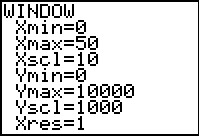
\includegraphics[width=1.75in]{./RationalsGraphics/Rationals12.jpg}  & 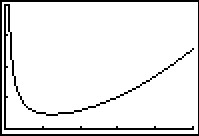
\includegraphics[width=1.75in]{./RationalsGraphics/Rationals13.jpg} & 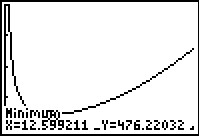
\includegraphics[width=1.75in]{./RationalsGraphics/Rationals14.jpg} \\


\end{tabular}
\end{center} 

\end{enumerate}
\qed

\end{ex}


\subsection{Variation}
\label{Variation}

In many instances in the sciences, rational functions are encountered as a result of fundamental natural laws which are typically a result of assuming certain basic relationships between variables.  These basic relationships are summarized in the definition below.

\smallskip

\colorbox{ResultColor}{\bbm

\begin{defn} \label{variation}  Suppose $x$, $y$ and $z$ are variable quantities.  We say

\begin{itemize}

\item  $y$ \index{variation ! direct}\index{direct variation}\textbf{varies directly with} (or is \textbf{directly proportional to}) $x$ if there is a constant $k$ such that $y=kx$.

\item  $y$ \index{variation ! inverse}\index{inverse variation}\textbf{varies inversely with} (or is \textbf{inversely proportional to}) $x$ if there is a constant $k$ such that $y=\frac{k}{x}$.

\item  $z$ \index{variation ! joint}\index{joint variation}\textbf{varies jointly with} (or is \textbf{jointly proportional to}) $x$ and $y$ if there is a constant $k$ such that $z = kxy$.


\end{itemize}

The constant $k$ in the above definitions is called the \index{variation ! constant of proportionality}\index{constant of proportionality}\textbf{constant of proportionality}.

\end{defn}

\ebm}

\smallskip

\begin{ex}  Translate the following into mathematical equations using Definition \ref{variation}.

\begin{enumerate}

\item  \href{http://en.wikipedia.org/wiki/Hooke's_law}{\underline{Hooke's Law}}:  \index{Hooke's Law} The force $F$ exerted on a spring is directly proportional the extension $x$ of the spring.

\item  \href{http://en.wikipedia.org/wiki/Boyle's_law}{\underline{Boyle's Law}}:  \index{Boyle's Law} At a constant temperature, the pressure $P$ of an ideal gas is inversely proportional to its volume $V$.

\item  The volume $V$ of a right circular cone varies jointly with the height $h$ of the cone and the square of the radius $r$ of the base.

\item  \href{http://en.wikipedia.org/wiki/Ohm's_law}{\underline{Ohm's Law}}:  \index{Ohm's Law} The current $I$ through a conductor between two points is directly proportional to the voltage $V$ between the two points and inversely proportional to the resistance $R$ between the two points.

\item \label{gravitylaw} \href{http://en.wikipedia.org/wiki/Law_of_universal_gravitation}{\underline{Newton's Law of Universal Gravitation}}:  \index{Newton's Law of Universal Gravitation} Suppose two objects, one of mass $m$ and one of mass $M$, are positioned so that the distance between their centers of mass is $r$.  The gravitational force $F$ exerted on the two objects varies directly with the product of the two masses and inversely with the square of the distance between their centers of mass.

\end{enumerate}

{\bf Solution.}  

\begin{enumerate}

\item Applying the definition of direct variation, we get  $F = k x$ for some constant $k$.

\item Since $P$ and $V$ are inversely proportional, we write $P = \frac{k}{V}$.

\item  There is a bit of ambiguity here.  It's clear that the volume and the height of the cone are represented by the quantities $V$ and $h$, respectively, but does $r$ represent the radius of the base or the square of the radius of the base?  It is the former.  Usually, if an algebraic operation is specified (like squaring), it is meant to be expressed in the formula.  We apply Definition \ref{variation} to get $V = k h r^{2}$.  

\item  Even though the problem doesn't use the phrase `varies jointly', it is implied by the fact that the current $I$ is related to two different quantities.  Since $I$ varies directly with $V$ but inversely with $R$, we write $I = \frac{k V}{R}$.

\item We write the product of the masses $mM$ and the square of the distance as $r^2$.  We have that $F$ varies directly with $mM$ and inversely with $r^2$, so $F = \frac{kmM}{r^2}$.  \qed

\end{enumerate}

\end{ex}

In many of the formulas in the previous example, more than two varying quantities are related.  In practice, however, usually all but two quantities are held constant in an experiment and the data collected is used to relate just two of the variables.  Comparing just two varying quantities allows us to view the relationship between them as functional, as the next example illustrates.

\begin{ex}  According to this \href{http://web.lemoyne.edu/~giunta/classicalcs/boyleverify.html}{\underline{website}} the actual data relating the volume $V$ of a gas and its pressure $P$ used by Boyle and his assistant in 1662 to verify the gas law that bears his name is given below.

\[ \begin{array}{|c||c|c|c|c|c|c|c|c|c|c|c|c|c|}  \hline

V & 48 & 46 & 44 & 42 & 40 & 38 & 36 & 34 & 32 & 30 & 28 & 26 & 24  \\ \hline

P & 29.13 & 30.56 & 31.94 & 33.5 & 35.31 & 37 & 39.31 & 41.63 & 44.19 & 47.06 & 50.31 & 54.31 & 58.81  \\ \hline \end{array} \]


\[\begin{array}{|c||c||c|c|c|c|c|c|c|c|c|c|c|c|} \hline

V & 23 & 22 & 21 & 20 & 19 & 18 & 17 & 16 & 15 & 14 & 13 & 12  \\ \hline 

P & 61.31 & 64.06 & 67.06 & 70.69 & 74.13 & 77.88 & 82.75 & 87.88 & 93.06 & 100.44 & 107.81 & 117.56   \\ \hline \end{array} \]

\begin{enumerate}

\item  Use your calculator to generate a scatter diagram for these data using $V$ as the independent variable and $P$ as the dependent variable.  Does it appear from the graph that $P$ is inversely proportional to $V$?  Explain.

\item  Assuming that $P$ and $V$ do vary inversely, use the data to approximate the constant of proportionality.

\item  Use your calculator to determine a `Power Regression' for this data\footnote{We will talk more about this in the coming chapters.} and use it verify your results in 1 and 2.


\end{enumerate}


{\bf Solution.}


\begin{enumerate}

\item If $P$ really does vary inversely with $V$, then $P = \frac{k}{V}$ for some constant $k$.  From the data plot, the points do seem to lie along a curve like $y = \frac{k}{x}$.

\item  To determine the constant of proportionality, we note that from $P = \frac{k}{V}$, we get $k = PV$.  Multiplying each of the volume numbers times each of the pressure numbers,\footnote{You can use tell the calculator to do this arithmetic on the lists and save yourself some time.} we produce a number which is always approximately $1400$.  We suspect that $P = \frac{1400}{V}$.  Graphing $y = \frac{1400}{x}$ along with the data gives us good reason to believe our hypotheses that $P$ and $V$ are, in fact, inversely related.

\begin{center}

\begin{tabular}{cc}

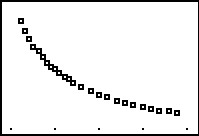
\includegraphics[width=2in]{./RationalsGraphics/Rationals15.jpg} \hspace{0.75in} & 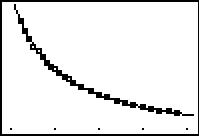
\includegraphics[width=2in]{./RationalsGraphics/Rationals16.jpg} \\

The graph of the data  \hspace{0.75in} & The data with $y=\frac{1400}{x}$ \\


\end{tabular}
\end{center} 



\item  After performing a `Power Regression', the calculator fits the data to the curve $y = ax^b$ where $a \approx 1400$ and $b \approx -1$ with a correlation coefficient which is darned near perfect.\footnote{We will revisit this example once we have developed logarithms in Chapter \ref{ExpLogs} to see how we can actually `linearize' this data and do a linear regression to obtain the same result.}  In other words, $y = 1400 x^{-1}$ or $y = \frac{1400}{x}$, as we guessed.


\begin{center}

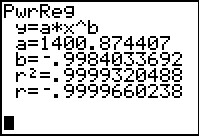
\includegraphics[width=2in]{./RationalsGraphics/Rationals17.jpg}

\end{center} 

\qed

\end{enumerate}

\end{ex}

\newpage

\subsection{Exercises}

In Exercises \ref{ratleqnexercisefirst} - \ref{ratleqnexerciselast},  solve the rational equation.  Be sure to check for extraneous solutions.

\begin{multicols}{2}
\begin{enumerate}

\item $\dfrac{x}{5x + 4} = 3$ \label{ratleqnexercisefirst}
\item $\dfrac{3x - 1}{x^{2} + 1} = 1$

\setcounter{HW}{\value{enumi}}
\end{enumerate}
\end{multicols}

\begin{multicols}{2}
\begin{enumerate}
\setcounter{enumi}{\value{HW}}

\item $\dfrac{1}{x + 3} + \dfrac{1}{x - 3} = \dfrac{x^{2} - 3}{x^{2} - 9}$
\item $\dfrac{2x + 17}{x + 1} = x + 5$

\setcounter{HW}{\value{enumi}}
\end{enumerate}
\end{multicols}

\begin{multicols}{2}
\begin{enumerate}
\setcounter{enumi}{\value{HW}}
\item $\dfrac{x^{2} - 2x + 1}{x^{3} + x^{2} - 2x} = 1$
\item $\dfrac{-x^{3} + 4x}{x^{2} - 9} = 4x$  \label{ratleqnexerciselast}

\setcounter{HW}{\value{enumi}}
\end{enumerate}
\end{multicols}

In Exercises \ref{ratlineqexercisefirst} - \ref{ratlineqexerciselast}, solve the rational inequality.  Express your answer using interval notation.

\begin{multicols}{3}
\begin{enumerate}
\setcounter{enumi}{\value{HW}}

\item $\dfrac{1}{x + 2} \geq 0$ \label{ratlineqexercisefirst}
\item $\dfrac{x - 3}{x + 2} \leq 0$
\item $\dfrac{x}{x^{2} - 1} > 0$

\setcounter{HW}{\value{enumi}}
\end{enumerate}
\end{multicols}

\begin{multicols}{3}
\begin{enumerate}
\setcounter{enumi}{\value{HW}}


\item  $\dfrac{4x}{x^2+4} \geq 0$
\item  $\dfrac{x^2-x-12}{x^2+x-6} > 0$
\item  $\dfrac{3x^2-5x-2}{x^2-9} < 0$

\setcounter{HW}{\value{enumi}}
\end{enumerate}
\end{multicols}

\begin{multicols}{3}
\begin{enumerate}
\setcounter{enumi}{\value{HW}}


\item  $\dfrac{x^3+2x^2+x}{x^2-x-2} \geq 0$
\item $\dfrac{x^{2} + 5x + 6}{x^{2} - 1} > 0$
\item $\dfrac{3x - 1}{x^{2} + 1} \leq 1$

\setcounter{HW}{\value{enumi}}
\end{enumerate}
\end{multicols}

\begin{multicols}{3}
\begin{enumerate}
\setcounter{enumi}{\value{HW}}

\item $\dfrac{2x + 17}{x + 1} > x + 5$
\item $\dfrac{-x^{3} + 4x}{x^{2} - 9} \geq 4x$
\item $\dfrac{1}{x^{2} + 1} < 0$ 

\setcounter{HW}{\value{enumi}}
\end{enumerate}
\end{multicols}

\begin{multicols}{2}
\begin{enumerate}
\setcounter{enumi}{\value{HW}}

\item $\dfrac{x^4-4x^3+x^2-2x-15}{x^3-4x^2} \geq x$
\item $\dfrac{5x^3-12x^2+9x+10}{x^2-1}\geq 3x-1$ \label{ratlineqexerciselast}

\setcounter{HW}{\value{enumi}}
\end{enumerate}
\end{multicols}

\begin{enumerate}
\setcounter{enumi}{\value{HW}}


\item  Carl and Mike start a 3 mile race at the same time.  If Mike ran the race at 6 miles per hour and finishes the race 10 minutes before Carl, how fast does Carl run?

\item  One day, Donnie observes that the wind is blowing at 6 miles per hour.  A unladen swallow nesting near Donnie's house flies three quarters of a mile down the road (in the direction of the wind), turns around, and returns exactly 4 minutes later.  What is the airspeed of the unladen swallow?  (Here, `airspeed' is the speed that the swallow can fly in still air.) 

\item  In order to remove water from a flooded basement, two pumps, each rated at 40 gallons per minute, are used. After half an hour, the one pump burns out, and the second pump finishes removing the water half an hour later.  How many gallons of water were removed from the basement?

\item  A faucet can fill a sink in 5 minutes while a drain will empty the same sink in 8 minutes.  If the faucet is turned on and the drain is left open, how long will it take to fill the sink?

\item Working together, Daniel and Donnie can clean the llama pen in 45 minutes.  On his own, Daniel can clean the pen in an hour.  How long does it take Donnie to clean the llama pen on his own?

\item  In Exercise \ref{newportaboycost}, the function $C(x) = .03x^{3} - 4.5x^{2} + 225x + 250$, for $x \geq 0$ was used to model the cost (in dollars) to produce $x$ PortaBoy game systems. Using this cost function, find the number of PortaBoys which should be produced to minimize the average cost $\overline{C}$.  Round your answer to the nearest number of systems. 

\item  Suppose we are in the same situation as Example \ref{boxnotopfixedvolume}.  If the volume of the box is to be $500$ cubic centimeters, use your calculator to find the dimensions of the box which minimize the surface area.  What is the minimum surface area?  Round your answers to two decimal places.

\item  The box for the new Sasquatch-themed cereal, `Crypt-Os', is to have a volume of $140$ cubic inches.  For aesthetic reasons, the height of the box needs to be $1.62$ times the width of the base of the box.\footnote{1.62 is a crude approximation of the so-called `Golden Ratio' $\phi = \frac{1 + \sqrt{5}}{2}$.}  Find the dimensions of the box which will minimize the surface area of the box.  What is the minimum surface area?  Round your answers to two decimal places.   

\item \label{fixedareaminperimetergarden} Sally is Skippy's neighbor from Exercise \ref{fixedperimetermaxareagarden} in Section \ref{QuadraticFunctions}.   Sally also wants to plant a vegetable garden along the side of her home.  She doesn't have any fencing, but wants to keep the size of the garden to 100 square feet.  What are the dimensions of the garden which will minimize the amount of fencing she needs to buy?  What is the minimum amount of fencing she needs to buy? Round your answers to the nearest foot. (Note:  Since one side of the garden will border the house, Sally doesn't need fencing along that side.)



\item Another Classic Problem: A can is made in the shape of a right circular cylinder and is to hold one pint. (For dry goods, one pint is equal to $33.6$ cubic inches.)\footnote{According to \href{http://dictionary.reference.com/browse/pint}{\underline{www.dictionary.com}}, there are different values given for this conversion.  We will stick with $33.6 \mbox{in}^{3}$ for this problem.}  

\begin{enumerate}

\item Find an expression for the volume $V$ of the can in terms of the height $h$ and the base radius $r$.
\item Find an expression for the surface area $S$ of the can in terms of the height $h$ and the base radius $r$.  (Hint: The top and bottom of the can are circles of radius $r$ and the side of the can is really just a rectangle that has been bent into a cylinder.)
\item Using the fact that $V = 33.6$, write $S$ as a function of $r$ and state its applied domain.
\item Use your graphing calculator to find the dimensions of the can which has minimal surface area.

\end{enumerate}

\item  A right cylindrical drum is to hold 7.35 cubic feet of liquid.  Find the dimensions (radius of the base and height) of the drum which would minimize the surface area.  What is the minimum surface area?  Round your answers to two decimal places.


\item In Exercise \ref{Sasquatchfunc1} in Section \ref{FunctionNotation}, the population of Sasquatch in Portage County was modeled by the function $P(t) = \frac{150t}{t + 15}$, where $t = 0$ represents the year 1803.  When were there fewer than 100 Sasquatch in Portage County?

\setcounter{HW}{\value{enumi}}
\end{enumerate}


In Exercises \ref{varexercisefirst} - \ref{varexerciselast},  translate the following into mathematical equations.

\begin{enumerate}
\setcounter{enumi}{\value{HW}}

\item  At a constant pressure, the temperature $T$ of an ideal gas is directly proportional to its volume $V$.  (This is \href{http://en.wikipedia.org/wiki/Charles's_law}{\underline{Charles's Law}}) \index{Charles's Law} \label{varexercisefirst}

\item  The frequency of a wave $f$ is inversely proportional to the wavelength of the wave $\lambda$.

\item  The density $d$ of a material is directly proportional to the mass of the object $m$ and inversely proportional to its volume $V$.

\item  The square of the orbital period of a planet $P$ is directly proportional to the cube of the semi-major axis of its orbit $a$. (This is \href{http://en.wikipedia.org/wiki/Kepler}{\underline{Kepler's Third Law of Planetary Motion }}) \index{Kepler's Third Law of Planetary Motion}

\item  The drag of an object traveling through a fluid $D$ varies jointly with the density of the fluid $\rho$ and the square of the velocity of the object $\nu$.

\item Suppose two electric point charges, one with charge $q$ and one with charge $Q$, are positioned $r$ units apart. The electrostatic force $F$ exerted on the charges varies directly with the product of the two charges and inversely with the square of the distance between the charges. (This is \href{http://en.wikipedia.org/wiki/Electrostatic#Coulomb.27s_law}{\underline{Coulomb's Law}}) \index{Coulomb's Law} \label{varexerciselast}

\setcounter{HW}{\value{enumi}}
\end{enumerate}

\begin{enumerate}
\setcounter{enumi}{\value{HW}}

\item According to \href{http://en.wikipedia.org/wiki/Vibrating_string}{\underline{this webpage}}, the frequency $f$ of a vibrating string is given by $f = \dfrac{1}{2L} \sqrt{\dfrac{T}{\mu}}$ where $T$ is the tension, $\mu$ is the linear mass\footnote{Also known as the linear density.  It is simply a measure of mass per unit length.} of the string and $L$ is the length of the vibrating part of the string.  Express this relationship using the language of variation.

\item According to the Centers for Disease Control and Prevention \href{http://www.cdc.gov}{\underline{www.cdc.gov}}, a person's Body Mass Index $B$ is directly proportional to his weight $W$ in pounds and inversely proportional to the square of his height $h$ in inches. \index{BMI, body mass index}

\begin{enumerate}

\item Express this relationship as a mathematical equation. \label{BMIfirst} 
\item If a person who was $5$ feet, $10$ inches tall weighed 235 pounds had a Body Mass Index of 33.7, what is the value of the constant of proportionality? \label{BMIsecond}
\item Rewrite the mathematical equation found in part \ref{BMIfirst} to include the value of the constant found in part \ref{BMIsecond} and then find your Body Mass Index.

\end{enumerate}

\item We know that the circumference of a circle varies directly with its radius with $2\pi$ as the constant of proportionality. (That is, we know $C = 2\pi r.$)  With the help of your classmates, compile a list of other basic geometric relationships which can be seen as variations.

\end{enumerate}

\newpage

\subsection{Answers}

\begin{multicols}{3} 
\begin{enumerate}

\item $x = -\frac{6}{7}$
\item $x = 1, \; x = 2$
\item $x = -1$

\setcounter{HW}{\value{enumi}}
\end{enumerate}
\end{multicols}

\begin{multicols}{3}
\begin{enumerate}
\setcounter{enumi}{\value{HW}}

\item $x = -6, \; x = 2$
\item No solution
\item $x = 0, \; x = \pm 2\sqrt{2}$

\setcounter{HW}{\value{enumi}}
\end{enumerate}
\end{multicols}

\begin{multicols}{2}
\begin{enumerate}
\setcounter{enumi}{\value{HW}}

\item $(-2, \infty)$
\item $(-2, 3]$

\setcounter{HW}{\value{enumi}}
\end{enumerate}
\end{multicols}

\begin{multicols}{2}
\begin{enumerate}
\setcounter{enumi}{\value{HW}}


\item $(-1, 0) \cup (1, \infty)$
\item $[0, \infty)$

\setcounter{HW}{\value{enumi}}
\end{enumerate}
\end{multicols}

\begin{multicols}{2}
\begin{enumerate}
\setcounter{enumi}{\value{HW}}

\item $(-\infty, -3) \cup (-3,2) \cup (4, \infty)$
\item $\left(-3, -\frac{1}{3} \right) \cup (2,3)$

\setcounter{HW}{\value{enumi}}
\end{enumerate}
\end{multicols}

\begin{multicols}{2}
\begin{enumerate}
\setcounter{enumi}{\value{HW}}

\item $(-1,0] \cup (2, \infty)$
\item $(-\infty, -3) \cup (-2, -1) \cup (1, \infty)$

\setcounter{HW}{\value{enumi}}
\end{enumerate}
\end{multicols}

\begin{multicols}{2}
\begin{enumerate}
\setcounter{enumi}{\value{HW}}

\item $(-\infty, 1] \cup [2, \infty)$
\item $(-\infty, -6) \cup (-1, 2)$

\setcounter{HW}{\value{enumi}}
\end{enumerate}
\end{multicols}

\begin{multicols}{2}
\begin{enumerate}
\setcounter{enumi}{\value{HW}}

\item $(-\infty, -3) \cup \left[-2\sqrt{2}, 0\right] \cup \left[2\sqrt{2}, 3\right)$
\item No solution

\setcounter{HW}{\value{enumi}}
\end{enumerate}
\end{multicols}

\begin{multicols}{2}
\begin{enumerate}
\setcounter{enumi}{\value{HW}}

\item $[-3,0) \cup (0,4) \cup [5, \infty)$
\item  $\left(-1,-\frac{1}{2}\right] \cup (1, \infty)$

\setcounter{HW}{\value{enumi}}
\end{enumerate}
\end{multicols}


\begin{multicols}{3}
\begin{enumerate}
\setcounter{enumi}{\value{HW}}

\item  4.5 miles per hour

\item  24 miles per hour

\item  3600 gallons

\setcounter{HW}{\value{enumi}}
\end{enumerate}
\end{multicols}

\begin{multicols}{3}
\begin{enumerate}
\setcounter{enumi}{\value{HW}}

\item  $\frac{40}{3} \approx 13.33$ minutes

\item 3 hours

\setcounter{HW}{\value{enumi}}
\end{enumerate}
\end{multicols}

\begin{enumerate}
\setcounter{enumi}{\value{HW}}

\item  The absolute minimum of $y=\overline{C}(x)$ occurs at $\approx (75.73, 59.57)$.  Since $x$ represents the number of game systems, we check $\overline{C}(75) \approx 59.58$ and $\overline{C}(76) \approx 59.57$.  Hence, to minimize the average cost, $76$ systems should be produced at an average cost of $\$59.57$ per system.

\item The width (and depth) should be $10.00$ centimeters, the height should be $5.00$ centimeters.  The minimum surface area is $300.00$ square centimeters.

\item The width of the base of the box should be $\approx 4.12$ inches, the height of the box should be $\approx 6.67$ inches, and the depth of the base of the box should be $\approx 5.09$ inches;  minimum surface area $\approx 164.91$ square inches.

\item The dimensions are  $\approx 7$ feet by $\approx 14$ feet;  minimum amount of fencing required $\approx 28$ feet.

\item 

\begin{multicols}{2}
\begin{enumerate}

\item $V = \pi r^{2}h$
\item $S = 2 \pi r^{2} + 2\pi r h$

\setcounter{HWindent}{\value{enumii}}
\end{enumerate}
\end{multicols}

\begin{multicols}{2}
\begin{enumerate}
\setcounter{enumii}{\value{HWindent}}

\item $S(r) = 2\pi r^{2} + \frac{67.2}{r}, \;$  Domain $r > 0$
\item $r \approx 1.749\,$in. and $h \approx 3.498\,$in. 

\end{enumerate}
\end{multicols}

\item  The radius of the drum should be $\approx 1.05$ feet and the height of the drum should be $\approx 2.12$ feet.  The minimum surface area of the drum is $\approx 20.93$ cubic feet.

\item $P(t) < 100$ on $(-15, 30)$, and the portion of this which lies in the applied domain is $[0,30)$.  Since $t=0$ corresponds to the year 1803, from 1803 through the end of 1832, there were fewer than 100 Sasquatch in Portage County.

\setcounter{HW}{\value{enumi}}
\end{enumerate}

\begin{multicols}{3}
\begin{enumerate}
\setcounter{enumi}{\value{HW}}

\item $T = k V$

\item \hspace{-.1in} \footnote{The character $\lambda$ is the lower case Greek letter `lambda.'} $f = \dfrac{k}{\lambda}$

\item $d = \dfrac{k m}{V}$ 

\setcounter{HW}{\value{enumi}}
\end{enumerate}
\end{multicols}


\begin{multicols}{3}
\begin{enumerate}
\setcounter{enumi}{\value{HW}}

\item $P^2 = k a^3$

\item \hspace{-.1in} \footnote{The characters $\rho$ and $\nu$ are the lower case Greek letters `rho' and `nu,' respectively.} $D = k \rho \nu^2$

\item \hspace{-.1in} \footnote{Note the similarity to this formula and Newton's Law of Universal Gravitation as discussed in Example \ref{gravitylaw}.}  $F = \dfrac{kqQ}{r^2}$   

\setcounter{HW}{\value{enumi}}
\end{enumerate}
\end{multicols}

\begin{enumerate}
\setcounter{enumi}{\value{HW}}

\item Rewriting $f = \dfrac{1}{2L} \sqrt{\dfrac{T}{\mu}}$ as $f = \dfrac{\frac{1}{2} \sqrt{T}}{L \sqrt{\mu}}$ we see that the frequency $f$ varies directly with the square root of the tension and varies inversely with the length and the square root of the linear mass.

\item \begin{multicols}{3} 
\begin{enumerate}
\item $B = \dfrac{kW}{h^{2}}$
\item \hspace{-.1in} \footnote{The CDC uses 703.} $k = 702.68$ 
\item $B = \dfrac{702.68W}{h^{2}}$
\end{enumerate}
\end{multicols}


\end{enumerate}


\closegraphsfile

\newpage

\end{document}